% -*- Mode:TeX -*-

%% The documentclass options along with the pagestyle can be used to generate
%% a technical report, a draft copy, or a regular thesis.  You may need to
%% re-specify the pagestyle after you \include  cover.tex.  For more
%% information, see the first few lines of mitthesis.cls.

%\documentclass[12pt,vi,twoside]{mitthesis}
%%
%%  If you want your thesis copyright to you instead of MIT, use the
%%  ``vi'' option, as above.
%%
%\documentclass[12pt,twoside,leftblank]{mitthesis}
%%
%% If you want blank pages before new chapters to be labelled ``This
%% Page Intentionally Left Blank'', use the ``leftblank'' option, as
%% above.

% singlespace

\documentclass[12pt,twoside,letterpaper]{mitthesis}
\usepackage{reader}
\usepackage{lgrind}
\usepackage[pdfborder={0 0 0}]{hyperref}
\usepackage{times}
\usepackage{graphicx}
\usepackage{listings}
\usepackage{fix-cm}
\usepackage[loose]{subfigure}
\usepackage{color}
\usepackage{footnote}
\usepackage{fancyhdr}
%\usepackage{git-info}

\input{vc}
\fancypagestyle{plain}{
    \fancyhf{} % clear all header and footer fields
    \fancyfoot[C]{\thepage} % except the center
    \fancyfoot[RO,LE]{\footnotesize DRAFT: \VCRevisionMod}%\gitinfo{@head}{commit}}
    \renewcommand{\headrulewidth}{0pt}
    \renewcommand{\footrulewidth}{0pt}
    }

\pagestyle{plain}

%% This bit allows you to either specify only the files which you wish to
%% process, or `all' to process all files which you \include.
%% Krishna Sethuraman (1990).

%\typein [\files]{Enter file names to process, (chap1,chap2 ...), or `all' to
%process all files:}
%\def\all{all}
%\ifx\files\all \typeout{Including all files.} \else \typeout{Including only \files.} \includeonly{\files} \fi

\begin{document}
\raggedbottom
% -*-latex-*-
% $Log: cover.tex,v $
% Revision 1.8  2008/05/13 15:02:15  jdreed
% Degree month is June, not May.  Added note about prevdegrees.
% Arthur Smith's title updated
%
% Revision 1.7  2001/02/08 18:53:16  boojum
% changed some \newpages to \cleardoublepages
%
% Revision 1.6  1999/10/21 14:49:31  boojum
% changed comment referring to documentstyle
%
% Revision 1.5  1999/10/21 14:39:04  boojum
% *** empty log message ***
%
% Revision 1.4  1997/04/18  17:54:10  othomas
% added page numbers on abstract and cover, and made 1 abstract
% page the default rather than 2.  (anne hunter tells me this
% is the new institute standard.)
%
% Revision 1.4  1997/04/18  17:54:10  othomas
% added page numbers on abstract and cover, and made 1 abstract
% page the default rather than 2.  (anne hunter tells me this
% is the new institute standard.)
%
% Revision 1.3  93/05/17  17:06:29  starflt
% Added acknowledgements section (suggested by tompalka)
%
% Revision 1.2  92/04/22  13:13:13  epeisach
% Fixes for 1991 course 6 requirements
% Phrase "and to grant others the right to do so" has been added to
% permission clause
% Second copy of abstract is not counted as separate pages so numbering works
% out
%
% Revision 1.1  92/04/22  13:08:20  epeisach

% NOTE:
% These templates make an effort to conform to the MIT Thesis specifications,
% however the specifications can change.  We recommend that you verify the
% layout of your title page with your thesis advisor and/or the MIT
% Libraries before printing your final copy.
\title{Tragedy of the routing table: An analysis of collective action amongst Internet network operators}

\author{Stephen Robert Woodrow}
% If you wish to list your previous degrees on the cover page, use the
% previous degrees command:
\prevdegrees{B.Sc. Computer Engineering, University of Manitoba (2007)}
% You can use the \\ command to list multiple previous degrees
%       \prevdegrees{B.S., University of California (1978) \\
%                    S.M., Massachusetts Institute of Technology (1981)}
\department{Engineering Systems Division \and Department of Electrical Engineering and Computer Science}

% If the thesis is for two degrees simultaneously, list them both
% separated by \and like this:
% \degree{Doctor of Philosophy \and Master of Science}
\degree{Master of Science in Technology and Policy \and Master of Science in Electrical Engineering and Computer Science}

% As of the 2007-08 academic year, valid degree months are September,
% February, or June.  The default is June.
\degreemonth{June}
\degreeyear{2011}
\thesisdate{May 6, 2011}

%% By default, the thesis will be copyrighted to MIT.  If you need to copyright
%% the thesis to yourself, just specify the `vi' documentclass option.  If for
%% some reason you want to exactly specify the copyright notice text, you can
%% use the \copyrightnoticetext command.
%\copyrightnoticetext{\copyright IBM, 1990.  Do not open till Xmas.}

% If there is more than one supervisor, use the \supervisor command
% once for each.
%\supervisor{Karen R. Sollins}{Principal Research Scientist, MIT CSAIL}
%\reader{David D. Clark}{Senior Research Scientist, MIT CSAIL}

\supervisor{Karen R. Sollins}{Principal~Research~Scientist,~Computer~Science~and~Artificial~Intelligence~Laboratory}
\reader{David D. Clark}{Senior Research Scientist,
Computer Science and Artificial Intelligence Laboratory}


% This is the department committee chairman, not the thesis committee
% chairman.  You should replace this with your Department's Committee
% Chairman.
\chairman{Leslie A. Kolodziejski}{Professor of Electrical Engineering \\ Chair, Department Committee on Graduate Students}
\director{Dava J. Newman}{Professor of Aeronautics and Astronautics and Engineering Systems \\ Director, Technology and Policy Program}

% Make the titlepage based on the above information.  If you need
% something special and can't use the standard form, you can specify
% the exact text of the titlepage yourself.  Put it in a titlepage
% environment and leave blank lines where you want vertical space.
% The spaces will be adjusted to fill the entire page.  The dotted
% lines for the signatures are made with the \signature command.
\maketitle

% The abstractpage environment sets up everything on the page except
% the text itself.  The title and other header material are put at the
% top of the page, and the supervisors are listed at the bottom.  A
% new page is begun both before and after.  Of course, an abstract may
% be more than one page itself.  If you need more control over the
% format of the page, you can use the abstract environment, which puts
% the word "Abstract" at the beginning and single spaces its text.

%% You can either \input (*not* \include) your abstract file, or you can put
%% the text of the abstract directly between the \begin{abstractpage} and
%% \end{abstractpage} commands.

% First copy: start a new page, and save the page number.
\cleardoublepage
% Uncomment the next line if you do NOT want a page number on your
% abstract and acknowledgments pages.
% \pagestyle{empty}
\setcounter{savepage}{\thepage}
\begin{abstractpage}
% $Log: abstract.tex,v $
% Revision 1.1  93/05/14  14:56:25  starflt
% Initial revision
% 
% Revision 1.1  90/05/04  10:41:01  lwvanels
% Initial revision
% 
%
%% The text of your abstract and nothing else (other than comments) goes here.
%% It will be single-spaced and the rest of the text that is supposed to go on
%% the abstract page will be generated by the abstractpage environment.  This
%% file should be \input (not \include 'd) from cover.tex.
In this thesis, I designed and implemented a compiler which performs
optimizations that reduce the number of low-level floating point operations
necessary for a specific task; this involves the optimization of chains of
floating point operations as well as the implementation of a ``fixed'' point
data type that allows some floating point operations to simulated with integer
arithmetic.  The source language of the compiler is a subset of C, and the
destination language is assembly language for a micro-floating point CPU.  An
instruction-level simulator of the CPU was written to allow testing of the
code.  A series of test pieces of codes was compiled, both with and without
optimization, to determine how effective these optimizations were.

\end{abstractpage}

% Additional copy: start a new page, and reset the page number.  This way,
% the second copy of the abstract is not counted as separate pages.
% Uncomment the next 6 lines if you need two copies of the abstract
% page.
% \setcounter{page}{\thesavepage}
% \begin{abstractpage}
% % $Log: abstract.tex,v $
% Revision 1.1  93/05/14  14:56:25  starflt
% Initial revision
% 
% Revision 1.1  90/05/04  10:41:01  lwvanels
% Initial revision
% 
%
%% The text of your abstract and nothing else (other than comments) goes here.
%% It will be single-spaced and the rest of the text that is supposed to go on
%% the abstract page will be generated by the abstractpage environment.  This
%% file should be \input (not \include 'd) from cover.tex.
In this thesis, I designed and implemented a compiler which performs
optimizations that reduce the number of low-level floating point operations
necessary for a specific task; this involves the optimization of chains of
floating point operations as well as the implementation of a ``fixed'' point
data type that allows some floating point operations to simulated with integer
arithmetic.  The source language of the compiler is a subset of C, and the
destination language is assembly language for a micro-floating point CPU.  An
instruction-level simulator of the CPU was written to allow testing of the
code.  A series of test pieces of codes was compiled, both with and without
optimization, to determine how effective these optimizations were.

% \end{abstractpage}

\cleardoublepage

\section*{Acknowledgments}

This is the acknowledgements section.  You should replace this with your
own acknowledgements.

%%%%%%%%%%%%%%%%%%%%%%%%%%%%%%%%%%%%%%%%%%%%%%%%%%%%%%%%%%%%%%%%%%%%%%
% -*-latex-*-

\pagestyle{plain}

\begin{singlespace}
      % -*- Mode:TeX -*-
%% This file simply contains the commands that actually generate the table of
%% contents and lists of figures and tables.  You can omit any or all of
%% these files by simply taking out the appropriate command.  For more
%% information on these files, see appendix C.3.3 of the LaTeX manual. 
\tableofcontents
\newpage
\listoffigures
\newpage
\listoftables


\end{singlespace}
\chapter{Introduction}
\label{chap:intro}

The autonomous and distributed nature of Internet networks, an intentional
consequence of the Internet architecture, can pose difficulty in coordinating
networks and their operators to achieve collective action. This observation is
visible in the slow progress being made on a number of the challenges that face
the Internet today: taking action against spam and malicious behavior,
transitioning to a larger Internet address space (IPv6), or adopting more
efficient network protocols. These are all cases where the costs and benefits
of individual action towards solutions are generally not commensurate, and so
no action takes place.

At the same time, the Internet has a relatively strong social network and sense
of community amongst its network operators---arguably a historical artifact
\cite{Mathew:2010ly}---that can be used to both promote and stigmatize
behaviors through social forces such as peer pressure and adherence to norms.
This has arguably been successful in achieving economically non-rational
behavior on the Internet\footnote{Cases of note include Stanford University
returning their /8 address block to IANA (``[A]s members of the network
community, we need to think about this issue and do the right thing.... It's
important for people that have large address space like ours to be good network
neighbors.'' \cite{Marsan:2000cr}), and more recently, Interop returning their
/8 address block to ARIN \cite{ARIN:2010nx}, as well as
organizing and participating in mutual aid efforts such as the Conficker
Working Group, DDoS mitigation, etc.}.
%, and perhaps even cases of collective action.
While these social forces are probably less strong than they once were when the
Internet was more homogeneous, and must now compete with commercial forces
stemming from providing Internet service as a business, they are still present
as any participant in a network operator community can attest to.

The purpose of this thesis is to investigate the effectiveness of one case
where social forces in the Internet operations community may have played a role
in mitigating an Internet collective action problem: the potentially
unsustainable growth of the Internet routing table. The objectives of this
investigation are twofold. The first is to understand whether the monitoring
mechanism that ostensibly spurred the social forces---the CIDR Report---was
effective in mitigating this problem. The second is to draw conclusions about
approaches to managing the Internet routing table (and possibly inform work on
other collective action problems affecting Internet operations and
infrastructure) based on lessons learned from analyzing the CIDR Report's
efficacy.
%
%These social forces may be useful and perhaps should be considered in
%designing solutions and building institutions to solve the challenges facing
%the Internet.

%%%%%%%%%%%%%%%%%%%%%%%%%%%%%%%%%%%%%%%%%%%%%%%%%%%%%%%%%%%%%%%%%%%%%%%%%%%%%%%%
\section{Context and motivation}

While invisible to most Internet users, interdomain routing is one of the
fundamental architectural elements of the Internet. Essentially the defining
characteristic of the Internet as a network of networks, interdomain routing
enables every network participating in the Internet to locate and exchange
traffic with every other Internet-connected network.

In the face of continued growth, the interdomain routing system used by
Internet networks faces scalability limits stemming from its design and
operation that can limit the ability of network service providers to build and
operate networks efficiently. The size and growth rate of the Internet routing
table, and specifically the number of prefixes in the table, is one of the
major sources of potential scaling issues \cite{rfc4984}. There are a number of
causes for this growth, including the addition of new customers and networks in
response to increased Internet demand and use, as well as network engineering
and the expression of routing policy for existing networks. As shown in Figure
\ref{fig:huston_table_plot}, the Internet routing table has grown at a
super-linear, sometimes exponential, rate over time \cite{Huston:2001bs}.

\begin{figure}[h]
\begin{center}
    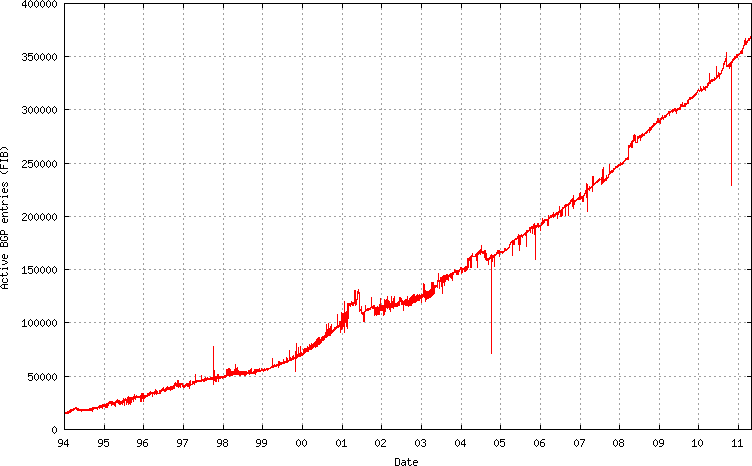
\includegraphics[width=4.5in]{static_figures/huston_table_plot.png}
    \caption[Size of the Internet (DFZ) routing table, 1994-present]
    {Growth of the Internet (DFZ) routing table, 1994-present
    \cite{6447-table-report}.}
    \label{fig:huston_table_plot}
\end{center}
\end{figure}

While the size of the routing table was once a serious concern of network
operators \cite{Li:2011vn}, engineering efforts have allowed the capabilities
of modern Internet routers to scale more quickly than the growth of the routing
table for the most part, allowing the Internet to continue to grow organically
without concern. Between evolutionary architectural improvements in succeeding
generations of Internet routers \cite{McKeown:2006kx} and the near-guaranteed
capacity and performance increases in semiconductors (i.e. Moore's Law), most
routers today have capacities that exceed the needs of the Internet routing
table. However, these engineering successes have not altered the underlying
scaling properties of BGP, the current interdomain routing protocol. While some
in the Internet engineering community claim that this is not a pressing concern
\cite{Huston:2011ys, Huston:2009dq}, others \cite{Li:2011vn} claim that the
lack of any mechanism to control or disincentivize routing table growth means
that there is no guarantee that routing table growth will not outpace
engineering developments in the future.

At present, table growth causes router vendors to make engineering trade-offs
\cite{Li:2011vn, Fall:2009fk} and requires planning and investment
consideration by network operators \cite{Zhao:2010fu}. While the actual size
and growth rate of the routing table has not exceeded the advances provided by
Moore's Law, it is exceeding Li's estimate of the constant cost sustainability
as shown in Figure \ref{fig:li_router_scalability}. Further, the related
challenges of IPv4 exhaustion, which will likely result in advertisement of
more, smaller address blocks due to address repurposing and transfers, and IPv6
adoption, which will drive growth of the IPv6 table\footnote{The IPv6 routing
table is still small (approximately 6000 prefixes), but currently appears to be
growing exponentially: \url{http://bgp.potaroo.net/v6/as6447/}} on dual-stacked
routers, may potentially cause routing table growth to accelerate towards a
point where routing becomes more expensive or even unsustainable (i.e.
outpacing Moore's Law). In the long term, unchecked growth could potentially
curtail the decentralized, laissez-faire growth and operation that has been a
hallmark of the Internet up to this point, or at the very least cause Internet
routing, and thus Internet service, to become more expensive than it presently
is.

% the theoretical\footnote{or even the more reasonable upper bound of
% $O(k\,2^{24})$ prefixes based on current RIR and operator policies} upper
% bound of $O(k\,2^{32})$ prefixes (where $k$ is a constant representing the
% number peers one connects to) is orders of magnitude beyond the capacity of
% any current router
\begin{figure}
\begin{center}
    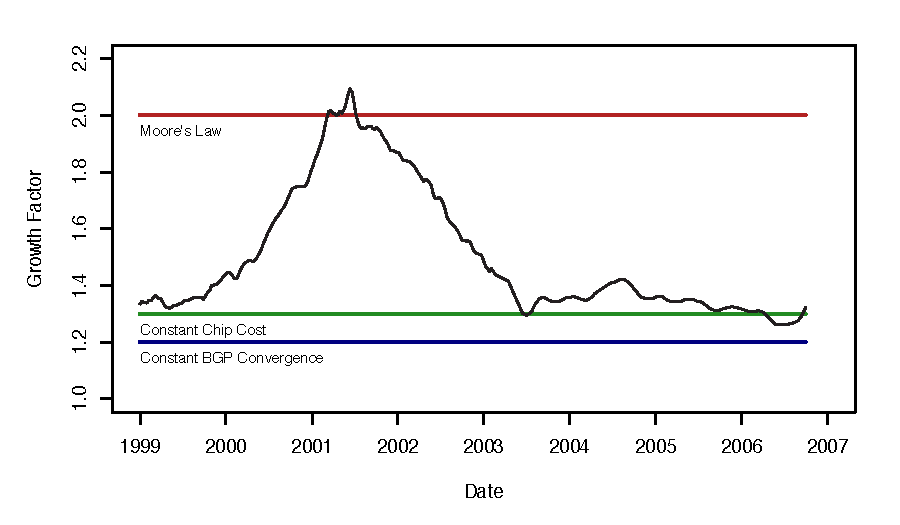
\includegraphics[width=6in]{static_figures/li_relgrowth.pdf}
    \vspace{-2em}\\
    \caption[Normalized growth factor of the Internet routing table relative
    to Moore's Law]{Normalized growth factor (smoothed over a 2 year window)
    of the Internet routing table relative to Moore's Law and other desirable
    engineering objectives, semiconductor chip cost and routing protocol
    convergence time, from 1999-2007 \cite{Li:2006cr}.}
    \label{fig:li_router_scalability}
\end{center}
\end{figure}

The specter of routing table scaling problems has been encountered once before
in the history of the Internet. In the early 1990s, as the Internet was
becoming more commercial and moving from a single hierarchical backbone to
multiple backbone providers, the Internet routing table began to grow at a rate
that would exceed the capabilities of routers available at the time
\cite{Huston:2001bs} and in some cases actually did affect the operational
behavior of the routers \cite{Li:2011vn}. The solution to this problem was
fundamentally a technical one: updating the addressing and routing architecture
of the Internet to allow networks to be aggregated, or advertised in larger
blocks, thus consuming fewer entries in the routing table. However, the
adoption of these technical protocol changes and improvements in operational
behavior required to enjoy benefit from these changes was promoted at least in
part by social forces within the operator community.

The mechanism that was used by the Internet operations community to promote
more efficient route advertisements was called the CIDR Report. Transmitted
weekly since the mid-1990s to mailing lists associated with major network
operator communities, the report contained a section called the ``aggregation
report'': an ordered list of the thirty networks that could most reduce the
number of entries in the Internet routing table by improving their route
announcement behavior. This email report was initially seen by network
operators as moderately successful in affecting network aggregation behavior,
but at some later point it came to be viewed as ineffective\footnote{Operator
views on the effectiveness of the CIDR Report come from correspondence with
Martin Hannigan, Patrick Gilmore, Tony Li \cite{Li:2011vn}, and Geoff Huston
\cite{Huston:2011ys}, as well as \cite{Steenbergen:2010nx}.}. It is interesting
that this social mechanism, one that superficially seems to provide only very
weak incentives and disincentives, was effective (at least as claimed by a
number of network operators and others in the community) in improving on this
collective action problem related to technology adoption and efficient route
announcement.

%%%%%%%%%%%%%%%%%%%%%%%%%%%%%%%%%%%%%%%%%%%%%%%%%%%%%%%%%%%%%%%%%%%%%%%%%%%%%%%%
\section{The case of the CIDR Report}

This thesis asks the question of whether the social forces in the Internet
operations community are capable of inducing collective action. This question
is asked in the context of one specific case: the CIDR Report and its ability
to control the growth of the Internet routing table. The working hypothesis for
this question is that appearing on the CIDR Report did not significantly affect
operator behavior. This position is based on discussions with network operators
and observation of the continually-increasing number of prefixes in the routing
table as shown in Figure \ref{fig:huston_table_plot}.

The case of the CIDR Report and routing table growth is of interest and
particularly well suited for this analysis for a number of reasons. First, this
case runs over a long period of time, starting in 1997, so there is a good
opportunity to observe community and individual operator behavior. This long
duration is backed by a large amount of publicly available data to support the
analysis of the report, including the CIDR Report emails themselves as well as
archived views of the Internet routing table. The CIDR Report is naturally
suited to allow for a quasi-experiment in that only part of the population is
``treated'' by the CIDR Report, while the rest of the population is available
for use as a control. Finally, the CIDR Report was and is a well-known and
well-publicized phenomenon within the operator community, and was created
with the intent of educating and also socially pressuring operators, and so
should be a suitable case for assessing the effects of social forces within
the Internet operator community.

Other potential cases involving the social forces within the operator
community, such as the back-channel communications mentioned in
\cite{Mathew:2010ly}, are difficult to study as there is typically a lack of
data, a lack of publicity of the events that occur that motivate social
pressure, and the events of potential interest for analysis are somewhat ad-hoc
and randomly distributed (e.g. the hijacking of YouTube by Pakistan Telecom
\cite{Brown:2008hc}).

% sentence here????

As with any study of a single case, it is generally not possible to make
generalizations about the broader question based the results of the study.
Thus, while this thesis is motivated by the potential use of social forces to
solve collective action problems of Internet operations, conclusions drawn from
my study of the CIDR Report may not be useful in providing insights for other
cases. However, any interesting insights about this case may be starting points
for further study and exploration in other cases.

%%%%%%%%%%%%%%%%%%%%%%%%%%%%%%%%%%%%%%%%%%%%%%%%%%%%%%%%%%%%%%%%%%%%%%%%%%%%%%%%
\section{The routing table as a Common Pool Resource}

The unconstrained growth of the Internet routing table is often considered a
commons problem: individuals derive private benefit from adding entries to the
table, but each entry incurs a public cost---a negative externality---for all
others that participate in the Internet routing system. The public cost is not
necessarily trivial either, with one network operator roughly estimating the
marginal cost of a BGP prefix at \$6000-\$8000 per year \cite{Herrin:2008qa}
and a researcher estimating the same figure at \$77,000 over the lifetime of
the router \cite{Clayton:2010bh}. This cost is not borne by any one network,
but is the estimated cost of the fraction of router resources consumed by one
route across all BGP-speaking routers with a full (DFZ) routing table
worldwide.

Discussions of the problem \cite{Huston:2001bs,Clayton:2010bh,Bellovin:2001qf}
often invoke Hardin's \cite{Hardin:1968uq} notion of the tragedy of the
commons---that individually rational actors will attempt to maximize
consumption of a resource because they privately enjoy the full benefit of this
consumption but share the cost of its reduced capacity, making all actors worse
off. Common solutions advocated for such problems are the establishment of a
central regulator or private property rights. However, the Internet routing
table and interdomain routing lacks both such features and has not yet been
reduced to tragedy. This is arguably a result, at least in part, of the
``property rights'' and governance regime of the interdomain routing system. By
understanding these characteristics, it may be helpful in understanding how and
why the CIDR Report had effect while also offering insights into other
approaches to enable more effective management of the routing table.

% TODO: MENTION THE BROADER ROLE OF INSTITUTIONAL ECONOMICS HERE?

In contrast to the broad notion of a ``commons problem'', Ostrom
\cite{Ostrom:1990fv} presents the more nuanced concept of common pool resources
(CPR) and CPR management problems. Her work has mostly focused on the
management of natural resources such as fisheries, forests, and aquifers, but
the general elements of the framework are applicable to other cases as well. In
Ostrom's model of common pool resources, the \emph{resource system} (such as a
fishery) is considered separately from the subtractable \emph{resource units}
(in this example, fish) that can be extracted from the resource. The resource
system produces some number of units that can be extracted sustainably, and
beyond that point extraction causes harm to the system itself. Actors that
extract resource units are referred to as \emph{appropriators} (fishers), and
actors that take efforts to improve or sustain the resource (such as farming
and stocking bodies of water with fish) are \emph{producers}. If the resource
system is not naturally occurring, then it must be created or organized by
\emph{providers}. In all cases, the essential defining qualities of a CPR are
that it is difficult to exclude others from using the resources (there are no
private property rights), and that the resource is rivalrous (the use of the
resource by one actor precludes its use by another).

The CPR framework can also be mapped relatively cleanly to the case of the
Internet routing table. The Internet's interdomain routing system is a CPR
resource system provided collectively by every network that maintains a router
with a full table of BGP routes.
%Operators of more popular or higher-traffic networks ostensibly must buy more
%equipment and thus pay a higher cost for their part of the system in order to
%meet demand, but in the case of content provider or ISPs this is often
%compensated for by payments (though based on traffic, not on routing table
%prefixes).
There is not a single global routing table---each provider maintains its own
version of the global routing table. However, the value in the routing table is
its consistency and uniqueness across all Internet participants in order to
allow global reachability. It is technically feasible for one network to
exclude others' routes from the routing table, but the utility of the
interdomain routing system comes from global reachability, and so it is
difficult to exclude routes without potentially reducing the utility of the
network's connectivity to the Internet.

Routing table capacity (``slots'' or routes) are the resource units of the
routing table CPR. Routing table entries are not intrinsically valuable in that
they cannot be ``extracted'' and used elsewhere. However, they are valuable in
that they permit interconnection and reachability to the rest of the Internet.
It is necessary for each network connected to the Internet to occupy at least
one slot in order to make the network available to the Internet, and its often
desirable to consume multiple slots for engineering or routing policy reasons.
Thus, networks must appropriate routing table slots to participate in the
Internet. These slots are rivalrous in that each router has a limited capacity
and slots used by one network's route announcements cannot be used by another.
As a public system with rival resource units, the interdomain routing system
has the hallmark characteristics of a CPR.

Mueller \cite{Mueller:2010bh} supports a similar view of the routing table as a
CPR, arguing that while IP addresses and address blocks could be handled as
private property, they are managed as common pool goods to protect the routing
table. He suggests that RIR address allocation policy is used to conserve
routing table slots by enforcing route aggregation and preventing IP address
block fragmentation that might result from reselling address blocks.

Under the CPR model, Ostrom's appropriators are rational individuals who make
decisions based on four inputs: the costs of a particular strategy, the
benefits of a particular strategy, their internal discount rate (the relative
perceived value of future benefits versus present benefits), and their internal
norms. What is notable about the appropriators in some CPR cases is that they
have learned about the limits of their resource system through trial and error
and, unlike the fictional rational grazers of Hardin's commons, communicate
with other appropriators to establish institutions that govern the
appropriation of units in an effort to ensure sustainability of the resource
system. Such institutions work to affect the decision-making algorithm of
appropriators by increasing the costs of a particular strategy through
sanctions, or establishing norms that are then internalized by the
appropriator, which in turn affect perceptions of costs and benefits.

% trust, small communities, etc.

CPR governance institutions---which usually include commitment to acceptable
behavior as well as mutual monitoring and sanction mechanisms to limit
opportunistic behavior---are not guaranteed to exist when a CPR is provided, or
to be effective even when they do exist. However, there is evidence that some
form of community-based governance institution has had an effect on the routing
table, such as Huston's observation of decreases in routing table size
following IETF meetings in the mid-1990s \cite{Huston:2001bs,Clayton:2010bh},
or the view of operators that the CIDR Report was effective in its early days.
In the case of the routing table, there are no explicitly obvious sanction
mechanisms beyond shame, criticism, and peer pressure of the network operator
community, which may affect the reputation of network providers and the
individuals operating their networks. Internalization of community norms of
cooperation and collegiality \cite{Abbate:2000ve} likely also contributed in
the case of the routing table.

In this context, the CIDR Report can be considered a mutual monitoring
mechanism that provided information about adherence to norms for the
loosely-defined, norm-based governance institution. It was not created or
mutually agreed upon by the community, but instead offered to the community by
a few individuals as part of the CIDR deployment effort, though its conclusions
could be verified by anyone with access to a router. The information provided
by the CIDR Report was embraced by some network operators as a basis for
invoking sanctions of shame and peer pressure that are sometimes visible on the
NANOG mailing list \cite{NANOG}, and it also affected operator behavior via
internal norms\footnote{In \cite{Li:2011vn}, Li notes that Cisco clients sought
advice and help to improve their route aggregation behavior after appearing on
the CIDR Report.}. However, as many operators have observed or conceded, the
CIDR Report appears to be less effective than it once was.

If we accept the view of the interdomain routing system and Internet routing
table as a CPR, and the CIDR Report as a monitoring mechanism for the
loosely-defined norms-based governance institution for the routing table, it
may be helpful to apply Ostrom's framework and analysis to the problem of
managing the routing table. The framework may be instructive in seeking to
understand the causes of variation in behavior change induced by the CIDR
Report over time that have caused operators to perceive the report as less
effective. Further, it may provide insights about other approaches to managing
the Internet routing table.

%%%%%%%%%%%%%%%%%%%%%%%%%%%%%%%%%%%%%%%%%%%%%%%%%%%%%%%%%%%%%%%%%%%%%%%%%%%%%%%%
\section{Contributions of this thesis}

This thesis makes a number of contributions to the space of Internet routing
table analysis, including:

\begin{itemize}
    \item{A history of the CIDR Report, as presented in Chapter
    \ref{chap:background}.}
    \item{A well-documented, open-source implementation of the CIDR Report
    aggregation report algorithm that utilizes multiple vantage points, as
    described in Chapter \ref{chap:method} and Appendix \ref{chap:opensource}.}
    \item{An analysis of the characteristics of the CIDR Report, including the
    distribution of appearances of networks on the report and the fraction of
    networks it treats, as presented in Chapter \ref{chap:analysis}.}
    \item{An analysis of the effects of appearing on the CIDR Report on the
    route announcement behavior of individual networks, also presented in
    Chapter \ref{chap:analysis}.}
    %\item{An analysis of network deaggregation behavior on a per-AS basis,
    %unlike other table-wide analyses.}
    \item{Consideration of the Internet routing table as a CPR and the CIDR
    Report as a monitoring mechanism for the CPR governance institution.}
\end{itemize}

%%%%%%%%%%%%%%%%%%%%%%%%%%%%%%%%%%%%%%%%%%%%%%%%%%%%%%%%%%%%%%%%%%%%%%%%%%%%%%%%
\section{Roadmap for remaining chapters}

The remainder of this thesis proceeds as follows. Chapter 2 presents a broad
overview of relevant background information in this space, both for the reader
who may be unfamiliar with interdomain routing or the Internet, as well as
those who wish to understand some of the finer points that motivate Internet
operations and routing table growth. This chapter also contains an overview
CIDR Report and a brief history of the events that motivated its creation and
evolution over time.

Chapter 3 describes the analytical approach taken to determine whether the CIDR
Report was effective. It begins by describing the data sources that were used
to conduct the analysis and the preprocessing steps taken against that data.
Next, the algorithms and methods used to generate the CIDR Report and its
aggregation report are described. Finally, the approach taken to analyze AS
behavior over time is presented and described.

Chapter 4 presents the results of this analysis: it first considers both the
overall characteristics of the CIDR Report and the networks that appear on it.
It then proceeds to a specific analysis of the route announcement behavior of
networks following an appearance on the CIDR Report, to determine if the CIDR
Report had an effect.

Following the presentation of these analytical results, Chapter 5 discusses the
meaning and implications of the results, as well reasons for why the efficacy
of the CIDR Report may have changed over time, by considering the routing table
growth situation through the lens of Ostrom's common pool resource framework.

Chapter 6 presents a review of related work from the literature and other
sources on measurement and analysis of the growth of the Internet routing
table, solutions to the scalability challenges facing interdomain routing, and
characteristics of the Internet operations community.

Finally, Chapter 7 offers a concluding discussion and recommendations regarding
the management of the Internet routing table, as well as how these observations
might be used to design institutions to solve other problems facing the
Internet, and suggestions for future research directions in this space.

\chapter{Background}

\section{Routing and Internet Operations}

\emph{NOTE: The following background is provided as a guide to the reader in order to discuss and articulate a number of the technical features of Internet routing and operations that are crucial to understanding this thesis, and which are relied upon extensively in the approach used to answer/analyze the thesis question. Advanced readers may wish to move forward to the following chapters on coordinating Internet operations and the CIDR Report, which contain much more specific background information relevant to the specific topic of this thesis.}

Interdomain routing (IDR) is essential to both the concept and operation of the Internet as a "network of networks". IDR enables the multitude of privately owned and operated networks that exist around the world to connect and exchange reachability information, which in turn enables a host connected in one network to contact another host connected to any other network. In the context of today's Internet, IDR is used to establish the topological location of blocks of network-layer identifiers---IP addresses---as well as routes to these blocks. This information allows routers within each network to send traffic destined for other networks in the appropriate "direction" in order to reach that network. The set of possible routes available for traffic from a network will be constrained by connectivity to other networks, as well as the commercial interests of Internet service providers who desire to route traffic to earn revenue or reduce costs.

This chapter begins with a broad overview of some of the fundamental aspects of IDR and the provision of Internet service from both a technical and a commercial perspective. From this foundation, the specific details of the Internet routing table and the protocol, BGP, used to establish it are discussed. Finally, commonly-used Internet operations activities that utilize BGP and thus affect the routing table are discussed.

\subsection{Interdomain Routing}

The interconnection of diverse networks was the fundamental design goal of the Internet \cite{Design Philosophies of the DARPA Internet Protocols}. While this goal prompted a number of design decisions that have resulted in the Internet as we know it today, the Internet's system of interdomain routing is one of the key operational elements of realizing this goal.

Routing generally refers to the process by which paths to specific destinations are determined, as well as the forwarding of incoming packets along the the previously-determined best path towards their ultimate destination. Each router need not know the entire path to every other destination on the network; the router simply passes the packet along to the next hop that has indicated that it knows the way to the destination. In this context, a route can be considered abstractly as a claim that the router announcing a route knows of a path that should deliver a message to a given destination, and is willing to deliver it to the next closest point in the path that it knows of.

Routing takes place at two scopes in networks today. First, \emph{intradomain} routing takes place within networks, the boundaries of which are typically demarcated by infrastructure ownership or policy (i.e. a business or campus network). Routes are typically established using dynamic interior routing protocols such as RIP, OSPF, ISIS, etc. The goals of interior routing are mainly to establish network-wide reachability efficiently, with little concern about the path taken. The presence of a route simply means that a link is up and can carry traffic. Operators may adjust metrics for links to balance traffic flow across networks, but there aren't many other concerns about which parts of the network know about or utilize which routes.

The second scope is between networks, such as the multitude of networks that interconnect to make the Internet. Unlike intradomain routing, \emph{interdomain} routing is focused on exchanging reachability information between various networks that are owned and operated with different policies and objectives. While reachability is still an important concern, other concerns relate to routing policy---the expression of desired behavior for network traffic. Routing policy is typically motivated by business concerns ultimately related to the carriage of traffic. In the context of interdomain routing, the exchange of routing information with another domain indicates a willingness to carry traffic to the route's destination. Thus, control of route announcements is important for business reasons. Routing policy objectives also include selective route advertisement in order to control traffic flow, as well as finer-grained capabilities to govern where traffic enters and exits a given network.

On the Internet, interdomain routing information is exchanged between \emph{autonomous systems} or ASes. These represent domains of consistent routing policy \cite{RFC1930}, and typically consist of a single organization's network, though complex network designs sometimes organize an organization's networks into multiple ASes for various reasons. Each AS is identified by a unique number, an AS Number, assigned to it by the IANA or the appropriate Regional Internet Registry. These identifiers are used as short-hand operational handles to refer to networks: MIT holds AS number 3, and AT\&T's north american backbone is often referred to as "AS 7018".

With the notion of a routes and autonomous systems defined, we can consider that the Internet abstractly as a directed graph with ASes as vertices and edges representing the willingness to carry traffic (according to the routes) for adjacent ASes. Let us now consider what the incentives are for ASes to interconnect, and the types of relationships this forms between networks as a result.

The value that comes from interconnecting networks is a sort of network effect---like other forms of communication, the Internet's value increases as the number of hosts reachable via the Internet increases. It is a long standing tradition on the Internet for pairs of networks that receive mutual benefit from interconnecting to do so without charging the other for the traffic sent. This practice is known as peering, and the pair of connecting networks would be considered to have a peer relationship. Peering is effective when the interconnecting networks derive similar benefits from the interconnection and when they are directly adjacent, but this is not often the case in the Internet. Unlike the case where peers gain benefit from connecting and providing access to each others users/customers, peers don't benefit when they carry traffic between two other peer ASes connected to it---what's known as providing \emph{transit} for those two networks. A different approach is required for networks that don't connect directly but that still wish to reach each other via the Internet.

Generally speaking, there are two ways for an autonomous system to receive routes that enable them to access the rest of the networks that compose the Internet. First, ASes may pay the other networks that they connect with to carry traffic to and from the rest of the Internet on the AS' behalf. Payment makes the carrying of traffic for others beneficial to interconnecting networks in cases where it normally wasn't in the previous discussion of peering. In these cases, the paying AS is a transit \emph{customer} of their upstream networks. Alternately, an AS operator can build its own network to have sufficient geographic breadth and presence in order to directly connect to other networks. This is a capital-intensive operation and so these networks are usually operated as businesses---network service \emph{providers}---to provide connectivity to other networks seeking connectivity to the Internet.

Each autonomous system is free to interconnect and exchange routing information with other networks as they choose, and many have their own unique policies in this regard. However, the generally-accepted logic is that routing policy is a rational decision-making process with the goal of maximizing income/minimizing payment. This can be distilled into a simple set of ordered preferences for selecting routes within a given AS. To reach a given prefix from a given AS, routes are preferred in the following order of availability:

\begin{enumerate}
    \item{Prefer a customer's route, as this allows the AS to charge the customer for this traffic.}
    \item{If a customer route is not available, prefer a peer's route as this allows the AS to send the traffic without charge.}
    \item{If a customer or peer route is not available, use the upstream provider's route. This is the route of last resort, as the AS must pay its provider for this traffic.}
\end{enumerate}

The upstream provider route is usually installed as a "default" route, which means it matches any prefix that the AS doesn't have specific routing information about on the assumption that the upstream provider has better connectivity to other networks than the AS. This is a reasonable assumption, especially for smaller networks at the edge of the Internet, and necessarily true for those that obtain connectivity from a single provider.

There is a small group of networks that are sufficiently large that they achieve reachability to all other Internet networks by using customer and peer routes. These networks are large providers that have many customers of their own, and who would never be customers of other large networks, resulting in peering relationships with their other large counterparts in order to reach the rest of the Internet. These networks do not have a default route, and are thus collectively known as the default-free zone (DFZ). The DFZ represents the "core" of the Internet, and its members have the most complete view of the Internet and play a significant role in Internet routing.

\subsection{The Border Gateway Protocol}

The Border Gateway Protocol (BGP) is the standard interdomain routing protocol that runs between networks to achieve Internet connectivity. The BGP specification defines a protocol for exchanging reachability information between autonomous systems, as well as an algorithm for selecting paths and means for expressing routing policy based on path advertisement and selection.

BGP operates as a bilateral session established between two BGP-speaking routers in adjacent autonomous systems. Once the session is established, network layer reachability information---IP address prefixes---that are known to each router is transmitted to the other AS' router, along with attributes corresponding to the prefixes, such as the origin, as-path, or the IP address of the next hop router for packets destined for that prefix. The routes advertised to ones neighbors may either originate from with the AS (for customers, infrastructure) or be from  other neighbors that one agrees to provide connectivity for. As the paths to prefixes change (such as when a link comes up or goes down), or as new prefixes are advertised or become unreachable, update messages are sent advertising or withdrawing routes accordingly. As route updates are received, the router updates its routing information base and may select and advertise a new best path based on this change in information.

A BGP route announcement might look like the following:

\fbox{figure of route announcement}
\begin{verbatim}
	route-views>show ip bgp 18.0.0.0/8
	BGP routing table entry for 18.0.0.0/8, version 5243
	Paths: (38 available, best #34, table Default-IP-Routing-Table)
	...
	  16150 3549 1239 3
	    217.75.96.60 from 217.75.96.60 (217.75.96.60)
	      Origin IGP, metric 0, localpref 100, valid, external
	      Community: 3549:2773 3549:31208 16150:63392 16150:65321 16150:65326
	...
\end{verbatim}

The AS-PATH feature of BGP is a distinguishing characteristic of the protocol and one of the most relevant characteristics of the protocol for the purposes of this thesis. It is constructed as announcements are received and reannounced by autonomous systems providing transit to each other. Each AS who announces a route appends their AS number to the AS-PATH of the prefix. This serves to provide loop prevention, as BGP speakers ignore routes with their own AS in their AS-PATH. The AS-PATH also serves as a source of topological information, identifying the AS that first announced the prefix---the origin AS---as well as the vantage point AS and the ASes in between. In the case of the AS-PATH from the announcement above, we can see that the prefix was originated by MIT (AS 3), observed by Phonera (AS 16150) and transited by MIT's upstream provider Sprint (AS 1239) and intermediate provider Global Crossing (AS 3549). By observing the AS-PATH information contained in a diverse set of routing tables, such as is visible from Route Views \cite{http://www.routeviews.org}, a great deal of information about connectivity and topology can be gleaned.

While generally not relevant to this discussion, BGP has a decision-making algorithm and tie-breaking procedure to use in consistently selecting the best path to a given prefix. What is perhaps important to note is that for forwarding traffic (as opposed to route selection), the most specific prefix that matches a given IP address will always take precedence. This is necessary to allow for subnetting, but is also what facilitates route hijacking.

Finally, routing policy can be controlled and expressed in a few ways with BGP. First, route advertisements incoming from neighbors may be filtered to ensure that the routes accepted into ones routing table agree with business and operational practices. Similarly, outgoing route advertisements to other neighbors may be filtered to ensure that internal routing policy is maintained (such as not providing transit to peers). Finally, operators may tag their outbound route announcements with "BGP communities". These are generally provider-specific attributes that affect the way providers will treat route announcements, such as prepending their AS-PATHs or only announcing them to part of their network. There are only a few well-known community attributes that are defined in RFCs, including the NO-EXPORT attribute which should instruct a peer to not share (export) the prefix with any of its neighbors.

\subsection{The Internet Routing Table}

The Internet routing table is where global Internet reachability information is collected and maintained by each autonomous system. Each AS will construct their routing table based on the connectivity with their neighbors and their own routing policy objectives. The Internet routing table can be constructed in a number of ways, including the manual configuration of routes by a router operator, but it is most commonly constructed by running BGP with one's neighbors to exchange reachability information.

While it's commonly referred to as "the" Internet routing table or the "global" routing table, there is no canonical definition of the routing table. Each AS will have it's own unique view of the Internet through its routing table because of that AS' unique position in the topology of the Internet. The AS' own policy requirements, as well as the routing policies of its neighbors will also affect the set of routes that it observes relative to other vantage points on the Internet. However, most ASes will have a roughly similar view of the Internet.

The Internet routing table is implemented as two sets of related data in most routers and as used by most networks. The main table of Internet routing information in an interdomain router is more precisely defined in the BGP specification \cite{BGP RFC} as the routing information base (RIB). Many routers also maintain a forwarding information base (FIB). All feasible routes received over all BGP sessions are stored in the router's RIB and remain there unless updated or withdrawn at a later time. Because the RIB may contain multiple possible routes for a given destination, it cannot be used directly for forwarding packets. Instead, the BGP path selection algorithm is run over the RIB to select the best path for each prefix. These best paths are then installed in the FIB where they are then used to forward packets to neighboring networks in order to reach their final destination. These best paths are also exported to any peers and customers of the AS, after filtering to enforce routing policy.

The FIB is typically a more compact version of the best paths in the RIB, and resembles a lookup table within each AS' border router that is used to determine the path along which incoming packets should be forwarded in order to reach their destination as specified in the IP packet header. An excerpt of what a routing table might look like is shown below:

\begin{tabular}{c | c | c}
    prefix & next\_hop & interface \\
    \hline
    ... & ... & ... \\
    10.0.0.0/8  & 192.168.10.1   & eth0 \\
	10.1.0.0/14 & 172.16.120.200 & eth1 \\
	10.2.1.0/24 & 172.16.120.204 & eth1 \\
    ... & ... & ...
\end{tabular}

For each incoming packet, the router searches the table for the longest, or most specific prefix, that matches the destination address and forwards the packet to the router specified by the address in the "next hop" column of the table. In the example above, a packet destined to 10.1.2.3 would be forwarded to the router at 172.16.120.200.

The resources within routers that are used to store the RIB and FIB and execute the BGP route selection algorithm are generally finite and fixed by the design of a given Internet router. The RIB in a routers' route processor DRAM, and the route processor CPU executes the BGP path selection algorithm on receiving a BGP update message from a peer. These routes are then installed in the FIB which is copied to high speed lookup memory (often content-addressable memory) associated with special packet forwarding processors on router linecards \cite{}. Given these limits, the scalability of the Internet is constrained to some degree by how its growth affects the size of the Internet routing table. The upper ceiling on router memory limits the absolute growth of the routing table in terms of the number of routes it can maintain. Each entry in a router's routing table memory is often coloquially referred to as a "slot". While this memory limitation is less of a problem in modern routers with multi-gigabyte memories and multi-million route capacities, this was a significant problem in early routers as the Internet began growing quickly in the early 1990s, with routers failing or behaving unusually as the routing table consumed all available memory. In contrast, router CPU utilization poses less of an absolute limit on routing table growth, but does cause other challenges. As the size of the routing table grows, the amount of data required to be processed for a large routing update or BGP session startup/reset has become significant. It is apparently not unusual for this initial router startup process to take tens of minutes \cite{NANOG RAS inconvenient prefix} before routes are exchanged with peers and connectivity is fully established. More generally, as the time required for processing routing updates increases, the time for routes to converge after a BGP update will also increase, resulting in poor performance and potential partial loss of Internet connectivity during transient network failures.

Concerns over the stability and scalability of Internet routing has made the growth of the routing table a topic of interest for at least the past two decades. A plot of the routing table over this time is shown below:

\fbox{figure plot from Geoff Huston, etc., of total prefixes over time.}

Its growth seems to be of less concern now given advances in router architecture and the continued performance improvement in semiconductor components keeping pace with Moore's Law \cite{Davie, Huston}. Interestingly, however, Tony Li claims that the growth of the routing table has forced router architects to make suboptimal design decisions about other aspects of router behavior in order to keep pace with this growth.

\subsection{Routing Policy And BGP Network Operations}

At its simplest and most efficient, the Internet routing table should contain one entry per autonomous system. Given that there are approximately 40,000 autonomous sytems visible on the Internet today, this would be a small and compact routing table, similar to that of the mid-late 1990s. However, the routing table cannot be made that simple for a number of reasons. The needs-based allocation policies used by RIRs \cite{RFC2050} to allocate blocks of IP addresses to end-user organizations results in fragmentation of IP address blocks and allocation of non-contiguous blocks to organizations as they receive new addresses over time. Such blocks cannot be announced from a single prefix, and so multiple routing table slots must be consumed to allocate each disjoint block allocated to an organization. Beyond fragmentation, most cases of increased consumption of routing table slots are the result of implementing routing policy for traffic incoming to a particular AS using the mechanisms available in BGP. A number of these mechanisms are discussed in turn below.

Control of routing policy for traffic exiting an AS is relatively straightforward---the AS operator simply needs to express and adjust their preferences for which route of those that they receive from their peers, customers, and providers should be selected for carrying that traffic to the specified prefix/destination. In contrast, managing routing policy for traffic entering an AS is much more difficult because selection of the best path for traffic originating from all other networks is dependent on factors such as AS-PATH length, etc. that the receiving AS lacks control over.

Many of the operational requirements of network service providers today regarding control over inbound traffic are not directly faciliated by explicit BGP features. Indeed, BGP provides only one "knobs" that an AS operator can adjust to influence its adjacent peers' path selection: the relatively limited multi-exit discriminator (MED) attribute \cite{O'Reilly BGP book?}. To achieve desired routing policy in more advanced situations such as multihoming and traffic engineering, operators must implement routing policy using other aspects of the BGP protocol. By understanding how the BGP path selection algorithm works and assuming that most peers follow the standard algorithm, an operator can implement more effective and fine-grained routing policy.

It is important to note that in general, each of these behaviors allows an AS to obtain private benefit by imposing a public cost against all other participants in the global routing system. To announce a multi-homed or traffic engineered network, which provides benefit to the operator initiating that behavior by allowing them to better manage their network, they necessarily add extra routes to the routing table of every network operator that collects a full routing table from their peers.

\paragraph{Multihoming}

Multihoming refers to the connection of a network to the Internet by more than one upstream provider. This is typically motivated by a desire for reliability, such that one will have network connectivity even in the event of a failure or misconfiguration on the part of an upstream provider. A basic approach to establishing connectivity for a multihomed AS would be to announce all of the AS' prefixes to all of the AS' upstream providers (sometimes referred to as anycasting). Depending on one's view of the Internet, a slot in RIB may be consumed for each of these announcements (i.e. for each of the upstream providers).

This will achieve the goal of multihoming, but may result in an imbalance of traffic between upstream links as distant ASes select the path to take based on factors that the origin AS likely doesn't have control over, such as the AS-PATH length. This can pose a problem if the AS' primary link is inexpensive and the backup link is expensive. The typical approach used to solve this problem is called AS-PATH prepending, where an AS will artificially lengthen their AS-PATH as observed by certain (i.e. high cost) providers in order to make specific links less attractive. Other issues regarding balance over links may arise, and these are best handled by the general class of behavior called traffic engineering.

\paragraph{Traffic Engineering}

Traffic engineering is the term for balancing traffic across network links to avoid runninoverloading links and allowing capacity for bursts, etc.

BGP network operations that affect the Internet routing table
       - poor advertisements
       - multihoming and traffic engineering
	- anycast
	- path prepending
	- cut-outs/more-specifics
       - hijacking prevention
       - prefix length filtering (and impacts on reachability therein)

\paragraph{Prefix Hijacking Prevention}

Prefix hijacking is the announcement of an IP address block by a network other than the legitimate owner of an address block. This can sometimes result from configuration errors \cite{Pakistan-Youtube} but can also be an intentional attack against a network \cite{DEFCON prefix hijack}. These attacks are particularly effective because routes with the longest matching prefix are selected, allowing the most specific prefix to "win" the traffic, even if its path is less optimal. To guard against the hijacking of address blocks, particularly for critical infrastructure such as authoritative name servers, some providers announce parts of their address blocks with the most specific prefix possible that they expect will be successfully pass global route filtering policy. This typically leads to the advertisement of /24 blocks for critical infrastructure. An example of which is show below, for Google's DNS servers, which are advertised as a /24 cut out of a /19 block.

\begin{verbatim}
	>dig google.com NS

	;; QUESTION SECTION:
	;google.com.			IN	NS

	;; ANSWER SECTION:
	google.com.		283561	IN	NS	ns1.google.com.
	...

	;; ADDITIONAL SECTION:
	ns1.google.com.		297490	IN	A	216.239.32.10
	...

	route-views>sh ip bgp 216.239.32.10
	BGP routing table entry for 216.239.32.0/24, version 360859
	...

	route-views>sh ip bgp 216.239.32.0/24 shorter-prefixes
	...
	   Network          Next Hop            Metric LocPrf Weight Path
	*  216.239.32.0/19  194.85.102.33                          0 3277 15169 i
	...
\end{verbatim}

\section{The CIDR Report and CIDR-ization of the Internet}

\subsection{Classless Interdomain Routing}

In contrast with individual end hosts which are fully identified by an IP address, there is also the need to refer to networks---collections of IP addresses which are connected together in a way that they are all reached by the same link.

\fbox{this is probably important to mention---the fact that the reason you define networks are to allow the abstraction in routing such that routers don't need to keep track of every end host.}

End hosts/devices connected to an IP network are fully identified by their IP address, which contains both the network address and the subnetwork address of that machine on the given network. The differentiation between the network and the subnetwork is given by partitioning the 32-bit IP address into a network part and subnet part, as shown in the figure below.

The original specification of the Internet Protocol implicitly encoded the size of the network in the first octet of the network address itself. Three classes were available: A, for large networks ($2^{24}$ hosts), B, for mid-sized networks ($2^{16}$ hosts), and C for small networks ($2^{8}$ hosts). Networks with the following first octet were assumed to be members of the class and thus be of that size. The distribution between A, B, and C networks was assumed by the protocol developers.

	\fbox{table of address blocks and allocations}

\begin{tabular}{ c | c | c | l }
    \textsc{Class} & \textsc{Address Range} & \textsc{Hosts/Network} & \textsc{Networks/Class} \\
    \hline
	A & 0.0.0.0--127.0.0.0         & $2^{24}$ & $2^{7}$ (128)               \\
	B & 128.0.0.0--191.255.0.0     & $2^{16}$ & $2^{14}$ (16384)            \\
	C & 192.0.0.0--223.255.255.0   & $2^{8}$  & $2^{21}$ (2097152)          \\
	D & 224.0.0.0--239.255.255.255 & \multicolumn{2}{l}{(224/4): multicast} \\
	E & 240.0.0.0--255.255.255.255 & \multicolumn{2}{l}{(240/4): experimental}
\end{tabular}

Assignment to permit use of these addresses by organizations was performed by the IANA, and addresses were allocated on a basis of justified need. Large organizations (like MIT, Ford, etc.) typically planned to, or were assumed to have large networks and many hosts, and so were granted class A addresses. Organizations that were somewhere in the middle would be granted a class B, and organizations expecting to have less than 254 hosts would get a class C. As networks grew, they would often be assigned new blocks rather than trading up to a larger block size---this was particularly frequent in the class C space. This issue of granting new class C blocks was also exacerbated by the realization that the class B block was the most commonly needed network size, yet was under-allocated compared to class C networks. As ASes with class C blocks needed to grow, they were allocated multiple class C blocks to conserve class B blocks.

Like all address blocks, each block allocated to a given AS needed to be announced to the Internet via the interdomain routing protocol, EGP and later BGP, in order to exchange traffic with other networks. Thus, each block occupied a slot in the routing table. As time wore on, particularly with the commercialization of the Internet and the transition from a single backbone to multiple backbones, the routing table began to grow to the point that it was causing problems with DFZ provider routers, particularly with hitting the ceiling of available DRAM in their routers, resulting in router failures and abnormal routing behavior \cite{tony li conversation}.

	\fbox{figure from cidr/big-internet working group}

The solution that was ultimately proposed to deal with this was route aggregation---the announcement of a single route that only occupied one routing table slot but covered multiple network blocks. Originally called supernetting \cite{RFC1338}, this was implemented by explicitly specifying the size of the network that was to be announced, and relaxing the previously hard boundaries specifying class A, B, and C. The deprecation of network address classes resulted in the final name of this effort, Classless Interdomain Routing, or CIDR. This was specified by the IETF in RFC 1519. Under CIDR, networks of any size could be announced, and these networks were now specified as a prefix and an explicit prefix length, typically specified in the format a.b.c.d/x. The prefix is the most significant bits of the network address that specify the network itself, and the length is the position of the partition between the network number and the subnetwork, implying the size of the subnetwork.

	\fbox{table showing translation from classful to classless addresses}

CIDR enabled aggregation of prefixes by combining multiple adjacent prefixes into larger networks. Route aggregation is the announcement of routes in a way that provides the same reachability as before aggregation while requiring fewer route announcements to do so. Take for example the case of announcing the block of addresses from 192.168.0.0--192.168.255.255. This could be announced with a single route (192.168.0.0/16), two routes (192.168.0.0/17, 192.168.128.0/17) or even 256 routes (192.168.0.0/24, 192.168.1.0/24, ..., 192.168.255.0/24). If these multiple prefixes are all originated by the same AS and carried to the greater Internet by the same providers, then then they provide the same connectivity and routing policy while consuming 1, 2, or 256 slots in the routing table. Thus, it is most efficient to announce address blocks as aggregated as possible.

	\fbox{figure of the different ways of announcing 192.168.0.0}

Determining how to announce blocks in aggregate can be done one of two ways. Adjacent, non-overlapping blocks issued by an RIR, such as the classful blocks allocated before CIDR, can be aggregated into a more specific covering prefix that is a synthetic announcement not corresponding to an RIR allocation. The other approach is to announce a less specific covering prefix that corresponds to all, or a larger part of, the classless block of addresses allocated by the RIR. In both cases, the more specific prefixes can then be withdrawn, achieving a net reduction in prefixes announced. An example of each of these approaches is shown below:

	\fbox{figure showing prefixes being aggregated into larger blocks by 1) synthesizing cover of adjacent blocks, and 2) announcing cover over small blocks}

With the specification of classless network addresses codified in the CIDR standard, the Border Gateway Protocol was updated to support this new method of representing networks in the context of network reachability information. The new version, version 4, of the protocol, sometimes referred to as BGP-4, was specified in YEARXXX, RFCYYYY.

The deployment of BGP4 required software and sometimes hardware upgrades to routers. BGP4-speaking routers were not compatible with BGP3-speaking routers, as the previous version of the protocol didn't support CIDR. This required some routers to speak both BGP4 and BGP3 to respective neighbors during the transition period to BGP4. Nevertheless, the transition was relatively quick in Internet time, taking about 2 years (according to Tony Li) and strongly motivated by the relief in stress from routing table growth that many network operators had been facing.

Even with the deployment of BGP4-speaking routers, aggregation did not automatically occur by the agency of software running on the routers. Instead, network operators needed to determine that their assigned address blocks were aggregable and then announce these aggregates "by hand". This did not always occur, especially for operators and a community that was used to speaking in terms of classful addresses. Thus, even with the necessary condition of BGP4 routers deployed, the potential savings through aggregation was not realized until network operators acted explicitly to reduce their route advertisements and the number of routing table slots they were consuming. It was this realization that drove the creation of the CIDR Report in the mid-1990s.

\subsection{The CIDR Report}

The CIDR report presents a summary of interesting routing table behavior related to routing table growth. The report contains a number of sections which have varied slightly over time, but it has always contained an overall summary of the size of the routing table over the past week, as well as the \emph{aggregation report}, which is of greatest interest for this thesis. The CIDR report is published via email every Friday to the major mailing lists that network operators participate in, including NANOG and similar lists in regions outside of North America. An excerpt of a recent CIDR Report is shown below:

	\fbox{figure CIDR report excerpt}

With each week's CIDR report, the aggregation report identifies the 30 ASes announcing the most aggregable routes, thus consuming slots in the global routing table that are unnecessary for the expression of routing policy. For the purposes of the aggregation report, an aggregable route is a route whose withdrawal would not cause a change in routing policy from the observer's (the CIDR Report host's) BGP vantage point.

Elements of the CIDR Report, and in particular the aggregation report, date back to approximately 1994-1995 when it was implemented by Cisco Systems employee Tony Bates. Bates was a member of the IETF's CIDR Deployment (CIDRD) working group, and the report was conceived to educate and motivate networks about the the transition to from classful to CIDR-aggregated route announcements with the advent of BGP4. The earliest reports available on the Internet date back to 1994, when it was referred to as the "Top 10" report \cite{ftp://ftp.ietf.org/ietf-online-proceedings/94jul/area.and.wg.reports/ops/cidrd/cidrd.bates.slides.ps}.

In mid-1996 the CIDRD group wound down \cite{ftp://ftp.ietf.org/ietf/cidrd/cidrd-minutes-96jun.txt}, and Tony transitioned the report to the NANOG mailing list. The first report still accessible on the Internet, collected from the NANOG mailing list archives \cite{URL...} dates from September 1996, when the report was briefly called the "Top-50" report. The report was soon renamed the CIDR Report and was issued weekly until August 2002 when responsiblity for the report was transferred to Geoff Huston of APNIC \cite{http://www.merit.edu/mail.archives/nanog/2002-08/msg00847.html}. The CIDR Report is still published every Friday (North American time zones) and has maintained a remarkably similar format over the 14 years where it can be observed on the NANOG mailing list.

\subsection{Implementation of the Aggregation Report}

The purpose of the aggregation report is to identify ASes announcing routes that could be more efficiently announced via aggregated route announcements without altering expressed routing policy. In the specific context of the CIDR Report, routing policy is simplified to mean inter-AS connectivity, captured via the AS-PATH for a given prefix. This is important for multihoming and some forms of traffic engineering, where it's necessary to announce more specific prefixes in addition to the covering prefix to allow traffic to be spread across multiple upstream providers instead of just taking the best route to the covering prefix. Without considering the fact that there is variation in one or more upstream ASes in the AS-PATH, these prefixes would be considered deaggregated even though they must be announced this way to achieve the desired routing policy.

Given this desire to respect routing policy, the aggregation report considers a prefix aggregable with another prefix if and only if the AS-PATHs match exactly. Aggregates are sought out using what appear to be two approaches in the aggregation report. \footnote{Note that I have received some form of source from Geoff Huston but it's difficult to interpret, so this is inferred based on my reading of the general and especially the detailed report for a single AS \cite{http://www.cidr-report.org/cgi-bin/as-report?as=AS6389&view=2.0}} First, more specific prefixes announced under a convering prefixes are checked for AS-PATH matches. If the paths match, the more specific prefix is withdrawn. An example of this behavior can be found in figure x.z. Second, the routing table is searched from more-specific to less-specific prefixes for adjacent prefixes with the same AS-PATH that can can be combined into a 1-bit less specific covering prefix, allowing the two more specific prefixes to be withdrawn. An example of this was shown earlier in figure x.y. The aggregation report also apparently aggregates across an adjacent "hole", or unannounced block, if there is no prefix below it. While this generally makes sense, it is potentially over-optimistic in that it doesn't consider RIR block allocations and the holes that may result from a block being allocated but unadvertised.

The number of advertised, aggregated, and withdrawn prefixes are totaled against the AS originating each of the prefixes, and these figures are exported to generate the CIDR Report, examples of which are shown below:

	\fbox{figure exceprt of detailed and general (emailed) cidr reports}

In these figures, 'current' or 'netsnow' refers to the total number of prefixes currently announced by the AS. 'withdrawn' refers to the number of prefixes that were able to be withdrawn after maximum aggregation. 'aggregated' refers to synthesized aggregate prefixes created by covering two adjacent prefixes. 'announced' or 'netsaggr' refers to total number of prefixes announced by the AS after maximum aggregation, and 'reduced' or 'netgain' refers to the total number of prefixes saved by the aggregation process; in other words, reduced is current less announced.

\fbox{mention how rank on CIDR Report is determined, and that the top 30 are all that are included}

The source of routing and (implicit) topology information in this case is from a provider's routing. This source/vantage point has varied over time, originally being measured from Xara.net, who had a connection to MAE East. This changed for a brief time to RouteViews before finally settling on APNIC R\&D who receives routing tables from ASX and AXY. In the case of APNIC and likely before then, the best path according to the router's BGP algorithm was selected for the analysis of a given prefix. This shouldn't generally be a problem, though potential cases such as the one below will result in a false deaggregation being claimed due to filtering, etc. on the part of one ISP.

\begin{verbatim}
	(example from email to geoff huston)

	Let's say peer A (AS 30) sees:

	10.0.0.0/8      30 20 10
	10.0.0.0/9      30 20 10
	10.128.0.0/9    30 20 10

	and peer B (AS 40) sees:

	10.0.0.0/8      40 10
	10.0.0.0/9      40 30 20 10
	10.128.0.0/9    40 30 20 10

	If you were to consider both peer's views, then you could aggregate 10/8's
	more specifics according to peer A but not according to peer B, and I was
	wondering how your algorithm decided whether 10/8's more specifics were
	aggregable for the CIDR report?

	In the case where you use the router's best path for a given prefix
	which is what it sounds like from your answer to my question about MOAS
	prefixes, I assume you might see something like this for the above
	prefixes:

	10.0.0.0/8      40 10
	10.0.0.0/9      30 20 10
	10.128.0.0/9    30 20 10
\end{verbatim}

As noted in the previous section about BGP network operations, a number of routing policy objectives are implemented via BGP using different aspects of the protocol. Some of these are visible via the AS-PATH, while others are not. Thus, the CIDR Report may not perfectly avoid altering intentional routing policy that's not captured via the AS-PATH.

Other potential problems include the fact that the provider of the view for the CIDR Report may present a slightly different view than they export---i.e. they send their unfiltered RIB best paths, which may result in the use of non-operational routes for generating the CIDR Report. Similarly, while the attribution of behavior to the origin AS generally makes sense, it's conceivable that route leaks/etc. may be caused by peers or upstream providers that do not obey BGP communities/no-export/etc. or who send this information to the CIDR Report vantage point in spite of it being filtered for actual operations. (Somehow explain that I expect Geoff Huston is competent enough to have a "good view" of the routing table, but that these are dilemmas regardless due to BGP) These and other potential dilemmas regarding the measurement and ground truth of interdomain routing behavior are discussed in the later discussion chapter.

NOTE: Geoff's policy of aggregating holes should prevent gaming (if only people cared enough to game the system) by advertising non-adjacent blocks

\subsection{Characteristics of the Aggregation Report}

(maybe this should go in the analysis?)
- distribution of ASes on the CIDR Report/aggregation report
- stratification of the report
- (total prefixes on cidr report/total prefixes in routing table), over time

\section{Coordinating Internet Operations}

Organizing and coordinating the Internet
       - historical note: originally some central coordination as an
         ARPA project, but still meritocratic and flat
       - ultimately little regulation, which means that "code is law"
         and people who control infrastructure can vote with their
         feet to varying extents
       - actors at play/with interests in the Internet space: vendors,
         operators, business users, consumer users,
         academics/researchers, governments, etc.
       - evolution of formal coordination of unique and high-value
         resources: ICANN, RIRs, etc.
       - evolution of information coordination of technical standards
         and best practices: IAB/IETF/IRTF, vendors roles in this, etc.
       - least formal coordination at the operations level — can even
         get to the point of "backdoor" communications (IRC, etc.)
         between ISPs to keep things running or to solve major problems
       - these are somewhat gathered in Internet operations community

Internet operator communities
       - NANOG is the canonical example, formed out of the NSFNET's
         regional techs mailing list
       - Other communities exist in various geographic regions —
         shared language, culture, and ability to meet is important,
         ad while Internet transcends geography to some degree these
         still can't be ignored
       - Typically provide a mailing list that carries a sizable
         contingent even though many more read than post, as well as
         meetings and other ways to share clue and communicate,
         network, make business deals/connections, etc.

\chapter{Analyzing the CIDR Report}
\label{chap:method}

This chapter describes the methods I employed to analyze the effectiveness of the CIDR Report. I begin with an overview of the analytical approach I designed and undertook, followed by the specific details of how I collected data and built the analytical tools to generate the data set that I analyze in the following chapter.

\section{Analytical Approach}

% be sure to avoid value-laden terminology within this

The general intuition in analyzing the effectiveness of the CIDR Report is relatively simple: \emph{do autonomous systems change their behavior, as measured by the number of aggregable routes they advertise into the routing table, after appearing on the CIDR Report?} If the hypothesis that the CIDR Report was effective in controlling routing table growth based on the social forces or reputation in the Internet operator community holds, then the behavior of ASes that appear on the CIDR Report should differ---becoming more aggregated---compared to the behavior of ASes that never appear on the CIDR Report. This can be viewed as a quasi-experiment \cite{Babbie:2003uq}, with ASes that appear on the CIDR Report composing the treatment group and ASes that never appear as the control group. This cannot be viewed as a true natural experiment or controlled experiment because the ASes in the treatment group are not randomly selected. The behavior that leads to appearance on the CIDR Report is typical of large ISPs and so they are disproportionally represented on the CIDR Report. This non-random appearance of ASes in the treatment group raise potential validity concerns, and the implications of this are discussed later.

The analysis of the performance of the treatment group could be implemented very simply by comparing the behavior of a given AS over time, starting when it first appears on the top thirty aggregation report. The CIDR Report emails transmitted to mailing lists weekly contain much of the information necessary to conduct this analysis. Accordingly, I first gathered and coded the data contained in these emails from network operator mailing list archives. This information determines which ASes are in the treatment group and when they appeared.

The CIDR Report emails have two shortcomings demand the gathering of additional data about the routing table. The aggregation report contains no information about ASes that do not appear within the top thirty, requiring other information to be gathered in order to form a control group. Also, rank (and thus appearance) is determined by relative ranking rather than absolute number of routes, and so an AS in the treatment group may leave the top 30 without aggregating simply because other ASes deaggregate more. In order to measure behavior in terms of routing table slots consumed by an AS, a non-truncated version of the CIDR Report is required. No archives of the full report are available, so I instead gathered historic routing table data and developed my own implementation of the aggregation report. The information from this generated aggregation report provides the metrics used for analysis of ASes in both the control and treatment groups for consistency.

Finally, utilizing the information from both the emailed (authoritative) CIDR Report and the full aggregation report generated from historic routing table data, I proceed with analysis, characterizing the overall behavior of ASes in the treatment and control groups, as well as behavior of ASes in both groups over time in order to observe whether the CIDR Report may have had an effect on treated AS' behavior.

\section{Data sources \& data collection} %%%%%%%%%%%%%%%%%%%%%%%%%%%%%%%

\subsection{Authoritative CIDR Reports}

The official CIDR Report has been transmitted weekly on Friday afternoons to network operator communities including the North American Network Operators Group (NANOG), starting in September 1997. The NANOG community has kept a public archive, \cite{NANOG} and \cite{NANOG-new}, of all messages sent to its mailing list since its inception in 1994, capturing all of the CIDR Report messages in its archive. This archive is an appropriate source of CIDR Reports as it contains the messages that were actually received by network operators (and so used to apply social force under the CIDR Report hypothesis).

The indexes of the archives were downloaded and parsed to obtain a set of message headers containing the sender name, subject, and date of all messages sent to the NANOG list. This message list was then filtered to create a coding candidate set containing only messages with a subject line containing "CIDR R" in any case.

The full bodies of the messages in the candidate set were downloaded from the NANOG archives for coding. The coding process consisted of viewing the message and classifying it as one of:

\begin{itemize}
\item{an official CIDR Report that appears to be correct,}
\item{an official CIDR Report that appears incorrect (duplicates, sent on the wrong date, containing obviously invalid data, etc.),}
\item{an email from the operator community praising, criticizing, or discussing behavior in the CIDR Report, or}
\item{none of the above (not of interest).}
\end{itemize}

Following the coding process, emails coded as official and correct CIDR Reports were parsed by an automated program to extract rank prefix count information for every AS appearing on the aggregation report. This information was then stored in a database for later use by other analysis tools.

One benefit of coding the authoritative CIDR Report emails by hand was that it enabled observation of changes in the CIDR Report's BGP data vantage point and implementation over time, as well as the transition of stewardship of the report. The report as originally conceived and implemented by Tony Bates was used from the first NANOG CIDR Report on 17 September 1996 until 23 August 2002. Geoff Huston then took responsibility for the report on 30 August 2002, producing a similarly-formatted report but with a new implementation that was developed without consulting Bates' source code \cite{Huston:2011ys}. The CIDR Report's vantage points over time are in the table below. The potential importance of vantage point selection is discussed further in Chapter \ref{chap:discussion}.

\savenotes
\begin{table}[h]
    \begin{center}
    \caption{CIDR Report vantage point ASes over time}
    \vspace{1em}
    \begin{tabular}{c | c | c}
        AS number & AS Name & Date effective \\
        \hline
        AS 5413 & Xara.net (at MAE-East) & 17 September 1996 \\
        AS 5413 & GX Networks & 15 June 2001 \\
        AS 6447 & Route Views & 30 August 2002 \\
        AS 4637 & REACH & 11 October 2002 \\
        AS 2.0 \footnote{AS 2.0 is not visible in the routing table, but peers with AS 4777 and AS 4608 \cite{Huston:2011ys}.} & APNIC R\&D & 20 July 2007 \\
    \end{tabular}
    \end{center}
\end{table}
\spewnotes

\subsection{Routing Table Data}

The University of Oregon Route Views project \cite{Routeviews} was used as the source of routing table data for generating a full aggregation report. Route Views gathers multiple views of the Internet routing table as seen by various major providers that peer with Route Views, and is a commonly used data source for operational and academic research. Route Views peers change over time, but typically include most of the default-free zone (DFZ) providers. The project has been storing routing table archives since November 1997.

Route Views' data sets export the entire Route Views RIB which contains all routes received from each provider it peers with. This differs from the Huston CIDR Report implementation \cite{Huston:2011ys} (and possibly from the original Bates CIDR Report implementation also), which used the best BGP route available instead of all routes available.

%The multitude of vantage points included in the Route Views data is arguably preferable in that it allows more potential aggregation to be visible to the CIDR Report algorithm, as discussed in the background section. It is also potentially problematic in that it includes ``leaked'' routes---routes not intended to be advertised globally---if they are advertised by even one provider. Discussion of the variation in routes observed from peers and the consequences of this---the potential importance of vantage point---are discussed later.

Route Views RIB snapshots are typically generated every two hours, and so a script was developed to search the archive indexes for the most appropriate snapshot to download in accordance with the CIDR Report's weekly Friday release schedule. The script selects the RIB snapshot created most recently after midnight each Friday. For the cases where RIB files were not found for a given Friday, the most recently generated RIB from earlier in the same week was selected instead. Between November 1997 and November 2001, snapshots in ``Cisco CLI''-format RIBs were downloaded from \url{route-views.routeviews.org}. After November 2001, MRT-format RIBs were downloaded from \url{route-views2.routeviews.org}. These RIBs were stored for preprocessing and ultimately the generation of the full aggregation report.

\section{Data preprocessing}

Several preprocessing steps are required to extract and normalize the data from the Route Views RIB files in order to prepare the data for use in generating the aggregation report.

First the information required from each RIB snapshot---namely the advertised prefix, the IP address of the observing peer, and the AS\_PATH associated with the route---are extracted from the snapshot files using RIPE's libbgpdump library \cite{libbgpdump} for MRT-format RIB snapshots and CAIDA's straightenRV tool \cite{straightenrv} for ``Cisco CLI''-format RIB snapshots. The output of these programs was a plain text representation of the information extracted from the RIB.

Next, these simplified RIB files were processed to canonicalize the AS\_PATH associated with each prefix. Since AS\_PATH equality is used by the aggregation report to determine whether the routing policy of two prefixes is the same, a canonical representation of the AS\_PATH is essential in order to allow AS\_PATH comparison. There are four steps in the canonicalization process:

\begin{enumerate}
\item{Removal of non-AS\_SEQUENCE elements in the AS\_PATH. AS\_SETs (denoted as \verb!{4,5}! for a set containing AS 4 and 5) can make the origin of a route ambiguous because there is not a single AS in the origin position of the AS\_PATH. To resolve such ambiguity, any AS\_SET is reduced to a single AS number if it contains only one AS number, or is discarded if it contain multiple unique AS numbers. AS\_CONFED\_SEQUENCEs (denoted as \verb![4 5]!) and AS\_CONFED\_SET (denoted as \verb!(4,5)!) should only contain private AS numbers and so are discarded without further consideration.

As an example of this transformation, the path \verb!1 1 1 2 3 (65535,65533) {4,4}! would become \verb!1 1 1 2 3 4!.
}

\item{Removal of private AS numbers. IANA has allocated private AS numbers \cite{rfc1930,rfc5398} for ISP internal use and documentation purposes, and these AS numbers sometimes appear in the Internet routing table. AS numbers within this range are removed from the AS\_PATH.}

\item{Removal of prepended AS numbers. As discussed earlier, AS\_PATH prepending is sometimes used by network operators to make a route appear less attractive to the BGP path selection algorithm. A prepended AS\_PATH affects traffic engineering but not routing policy, and so prepended AS numbers are removed by collapsing contiguous blocks of the same AS number into a single entry in the AS\_PATH.

For example, the path \verb!1 1 1 2 3 3 4! would be collapsed to \verb!1 2 3 4!.}
\item{Removal of simple routing loops. Minor routing loops sometimes occur in the BGP routing table, such as when a route traverses a provider that uses multiple AS numbers for different parts of their infrastructure. These loops are removed following the algorithm used by CAIDA in straightenRV\cite{straightenrv}. If a more complex loop is found that cannot be resolved using this algorithm, the entire route is discarded.

For example, the path \verb!1 2 3 2 5!, which may have resulted from AS 2 and 3 belonging to the same operator, is reduced to \verb!1 2 5!. In contrast, a more complex loop such as \verb!1 2 3 2 3 4! cannot be resolved using CAIDA's heuristic.}
\end{enumerate}

Finally, because this canonicalization process requires a full traversal of the input RIB in order to produce the canonical RIB, other data sets can be opportunistically generated during the canonicalization process. The number of prefixes observed by each Route Views peer are recorded, for each origin AS and for the entire routing table, to allow later analysis of variation in the prefixes seen per peer. This information was a helpful debugging tool and will also be used for the later discussion of the consequences of vantage point selection.

\section{Implementing the Aggregation Report}

Determining which prefixes in a RIB are aggregable consists of three major steps. First, a prefix tree data structure containing all advertised prefixes is constructed in order to establish which prefixes are adjacent to and covered by other prefixes. Next, the tree is walked recursively aggregate adjacent prefixes and to classify prefixes that may be aggregated by a covering prefix, both only in cases where routing policy is not compromised. Finally, counts of aggregable and total prefixes are attributed to each origin AS. These counts are then ranked to generate the aggregation report as seen on the CIDR Report. Each of these steps is described in more detail below.

To construct the binary prefix tree (technically a binary prefix trie, \cite{Wu:2008fk}) containing a set of prefixes that we wish to aggregate over, we must first determine the root of the tree. If prefixes of any length were allowed then the tree would need to be rooted at 0.0.0.0/0. However, because IANA has always allocated IP address blocks as Class A or /8 blocks, we can generate the aggregation report by considering each /8 separately. Taking advantage of this fact will make the implementation of the classification algorithm more efficient as the entire routing table need not be stored in memory. Accordingly, the input RIB will be sorted on the first octet of the prefix and processed by the algorithm one /8 at a time.

For each /8, a prefix tree will be constructed with the root at the the /8 prefix (for example, 10.0.0.0/8). Then each prefix in the RIB, as observed by each peer, is inserted into the tree. Each node contains a prefix, the corresponding AS\_PATH for that prefix, and pointers to the two more specific sub-prefixes of the current prefix if they exist. An small example of a prefix tree is shown in Figure \ref{fig:ex_prefix_tree}.

\begin{figure}
\begin{center}
    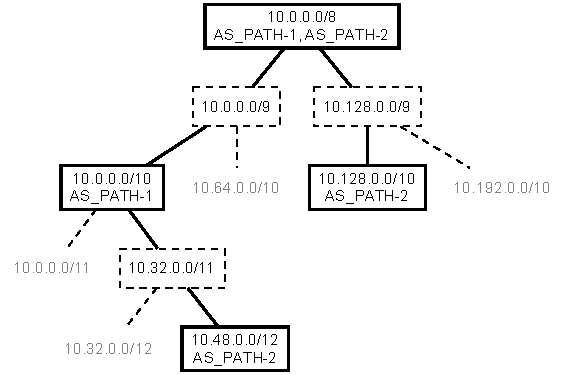
\includegraphics{figures/ex_prefix_tree.pdf}
    \caption[A prefix tree]{A prefix tree for 10.0.0.0/8 and some more specific prefixes. Prefixes with solid borders and AS\_PATHs are announced in the routing table, and prefixes with dashed borders are placeholders.}
    \label{fig:ex_prefix_tree}
\end{center}
\end{figure}

To insert a prefix into the tree, a cursor is placed at the root and then advanced to one of the two children of the root depending on whether the first bit after the first octet of the IP prefix is a `1' or a `0'. This process is then repeated recursively from the current node for each subsequent bit in the prefix. If at any point a node does not have a child must be traversed to reach the insertion point, a placeholder prefix is inserted to maintain the tree structure. When the depth in the tree is equal to the length of the prefix less the original eight bits of the /8, the prefix is inserted into the tree. The insertion process is illustrated in Figure \ref{fig:ex_prefix_tree_insert}.

\begin{figure}
    \subfigure[Bit 9 of the prefix is a `1', so the cursor proceeds to the `1' child.]
        {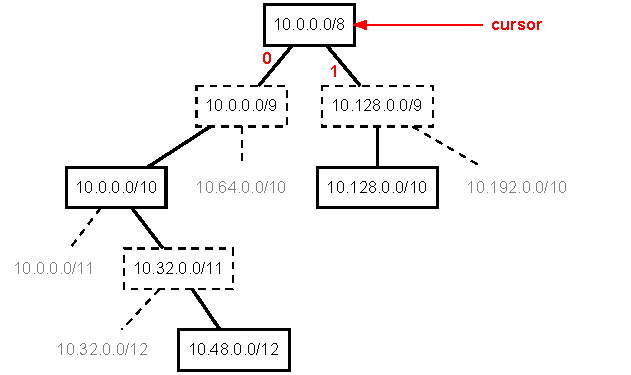
\includegraphics[width=3in]{figures/prefix_insert_gl1.pdf}}
    \subfigure[Bit 10 of the prefix is a `0', so the cursor proceeds to the `0' child.]
        {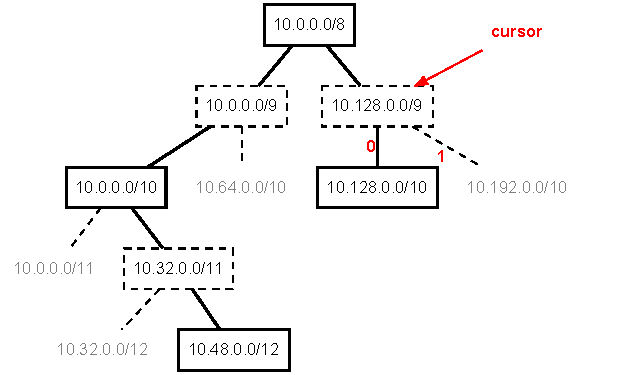
\includegraphics[width=3in]{figures/prefix_insert_gl2.pdf}}
    \subfigure[Bit 11 of the prefix is a `1', so the cursor proceeds to the `1' child. The `1' child does not exist, so a placeholder prefix is inserted as the `1' child.]
        {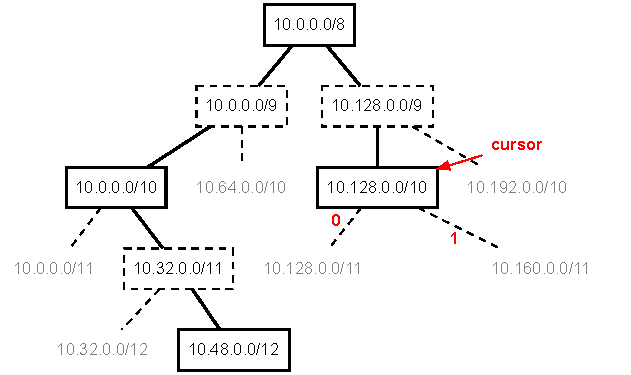
\includegraphics[width=3in]{figures/prefix_insert_gl3.pdf}}
    \subfigure[Bit 12 of the prefix is a `0', so the cursor proceeds to the `0' child. The `0' child does not exist. Since the current bit is equal to the prefix length (/12) the (non-placeholder) prefix 10.160.0.0/12 is inserted as the `0' child.]
        {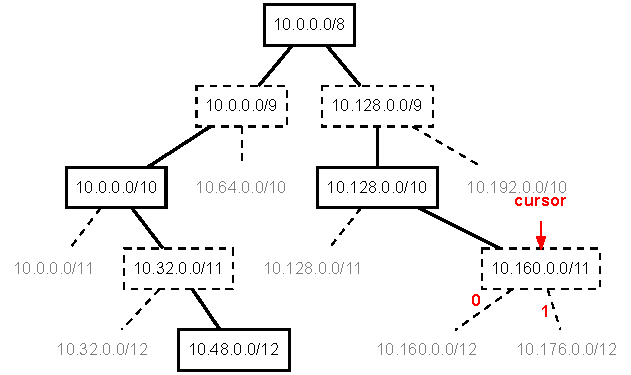
\includegraphics[width=3in]{figures/prefix_insert_gl4.pdf}}
    \subfigure[Insertion of 10.160.0.0/12 is complete.]
        {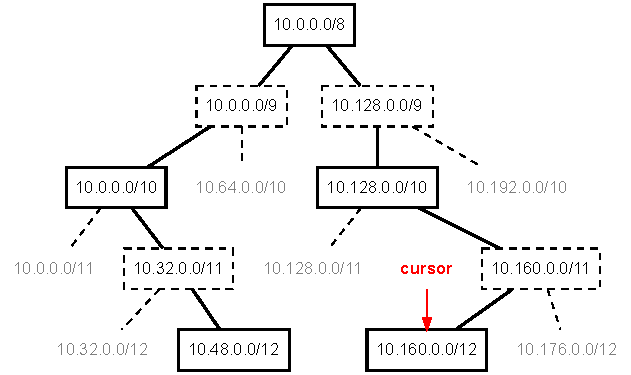
\includegraphics[width=3in]{figures/prefix_insert_gl5.pdf}}
    \caption[Insertion into the prefix tree]{Insertion of 10.160.0.0/12 into the prefix tree described in Figure \ref{fig:ex_prefix_tree}. Recall that 10.160.0.0 is represented as 00001010.10100000.00000000.00000000 in binary.}
    \label{fig:ex_prefix_tree_insert}
\end{figure}

Unlike the Huston and likely the Bates implementations of the aggregation report, this implementation considers all routes available from all peers for a given prefix in the routing table, instead of just the best route. Thus, for a given prefix in the tree, there are actually multiple AS\_PATHS stored---one for each peer that observes the route. This can be viewed logically as several prefix trees overlaid on top of each other, though the implementation uses a single tree with multiple AS\_PATHs per prefix. All distinct AS\_PATHs for a given prefix are gathered from the input RIB and associated with the prefix before it is installed in the prefix tree.

%This is important in that it allows the most potential aggregation to be observed because it does not conflate routes viewed from different peers. For example, consider the following topology shown in Figure \ref{fig:ex_topology}, and the routes observed from two peers shown in the routing table below:
%
%\begin{figure}
%\caption{Example topology and route announcements.}
%\label{fig:ex_topology}
%\end{figure}
%
%% \begin{tabular}{l | l}
%%     prefix        & AS\_PATH \\
%%     \hline
%%     10.0.0.0/8    & 30 20 10 \\
%%     10.0.0.0/9    & 30 20 10 \\
%%     10.128.0.0/9  & 30 20 10 \\
%% \end{tabular}
%%
%% \begin{tabular}{l | l}
%%     prefix        & AS\_PATH \\
%%     \hline
%%     10.0.0.0/8    & 40 10       \\
%%     10.0.0.0/9    & 40 30 20 10 \\
%%     10.128.0.0/9  & 40 30 20 10 \\
%% \end{tabular}
%%
%% \begin{tabular}{l | l}
%%     prefix        & AS\_PATH \\
%%     \hline
%%     10.0.0.0/8    & 40 10    \\
%%     10.0.0.0/9    & 30 20 10 \\
%%     10.128.0.0/9  & 30 20 10 \\
%% \end{tabular}
%
%\begin{figure}
%\caption{Example routing tables based on routes and topology in figure \ref{fig:ex_topology}}
%\label{fig:ex_tables}
%\begin{centering}
%\begin{tabular}{l | l c l | l c l | l}
%    \multicolumn{2}{c}{\textsc{Routes From AS 30:}} & & \multicolumn{2}{c}{\textsc{Routes From AS 40:}} & & \multicolumn{2}{c}{\textsc{Observer's Best Routes:}} \\
%    prefix        & AS\_PATH & & prefix       & AS\_PATH    & & prefix & AS\_PATH \\
%    \cline{1-2} \cline{4-5} \cline{7-8}
%    10.0.0.0/8    & 30 20 10 & & 10.0.0.0/8   & 40 10       & & 10.0.0.0/8 & 40 10 \\
%    10.0.0.0/9    & 30 20 10 & & 10.0.0.0/9   & 40 30 20 10 & & 10.0.0.0/9 & 30 20 10 \\
%    10.128.0.0/9  & 30 20 10 & & 10.128.0.0/9 & 40 30 20 10 & & 10.128.0.0/9 & 30 20 10 \\
%\end{tabular}
%\end{centering}
%\end{figure}
%
%By looking at only the BGP-selected best routes from the observation vantage point (the right-most table in Figure \ref{fig:ex_tables}), it's possible to conclude that routes aren't aggregable.

Once all of the prefixes in the RIB for the current /8 are inserted into the prefix tree, the prefix tree is walked recursively to aggregate and classify aggregable prefixes within the tree. As noted in the background, a prefix is considered aggregable if it has the same routing policy as a less-specific covering prefix. The aggregation and classification algorithm was implemented based on the description of the CIDR Report included in the Report's preamble, as well as detailed records of the report's operation \cite{cidr-report-details}. Like the authoritative CIDR Report, routing policy equality in this implementation of the aggregation report is determined by comparing AS\_PATH equality.

The general algorithm behind the aggregation and classification process is as follows. The prefix tree is traversed using post-order recursion and the following operations are performed on each node before the function returns to its calling parent (the post-order traversal ensures that children are aggregated before their parents):
\begin{enumerate}
\item{Attempt to aggregate children: If the current prefix is a placeholder and has two more-specific (child) prefixes announced in the routing table, check to see if their AS\_PATHs match. If they do, convert the current prefix into a ``true'' (non-placeholder) prefix and mark the children prefixes as aggregable.}
\item{Attempt to aggregate by a covering prefix: Compare the AS\_PATH of the current prefix with the AS\_PATH of its nearest less-specific (ancestor) prefix . If they match, mark the current prefix as aggregable.}
\end{enumerate}

%A small example is show in figure
%
%\begin{figure}
%\label{fig:ex_aggregation}
%\caption{An example of the aggregation process}
%\end{figure}

This process is again logically conducted as though there are multiple separate but overlaid trees for each Route Views peer/observer AS. The process is actually implemented by processing all vantage points available at a given prefix and aggregating and classifying them against other ancestor and child prefixes visible from the same peer AS. Classifications of aggregability are made on a per-peer basis, and then must be generalized for the entire prefix. There is no single way to make this generalization and so a design decision must be made.

There are two obvious choices for how generalize across each vantage point's aggregation classification for a given prefix: consider the prefix aggregable if \emph{any} vantage point considers it aggregable, or only if \emph{all} vantage points consider it aggregable. The latter option requires consensus that a prefix be aggregable across all views, while the former allows any claim of aggregability to stand. This implementation of the aggregation report classifies a prefix as aggregable if it is classified as aggregable from \emph{any} vantage point. While perhaps ``pessimistic'', this approach will detect and report the maximum amount of aggregation potentially possible.

%\fbox{include note on multihoming/traffic engineering, and whether this applies as compared to other efforts., i.e. citadinni}

Finally, when a prefix is marked as aggregable, it must be attributed to the network that announced the prefix as this network is responsible for the redundant route announcement. This is normally performed by attributing the aggregable route to the origin AS---the first AS in the route's AS\_PATH---that is presumed to be the announcing network. An ambiguous situation arises in the case of prefixes announced by multiple ASes, a condition known as a multiple origin AS (MOAS) \cite{Zhao:2001ly}. Again, a design decision must be made for how to attribute aggregable MOAS prefixes: the MOAS prefixes could be ignored, the route's behavior could be attributed to one of the origin ASes, or it could be attributed to all origin ASes. This implementation attributes an aggregable prefix to each unique AS that announces the prefix.

To attribute deaggregation behavior to each AS, the aggregation report processor maintains three quantities for each origin AS:

\begin{itemize}
\item{Announced routes: routes that were originally announced in the input RIB. This is the ``netsnow'' quantity in the aggregation report}
\item{Withdrawn routes: routes that were covered by less specific routes and thus would be withdrawn from the ideally-aggregated routing table.}
\item{Aggregated routes: routes that did not exist in the original routing table, but were synthesized by combining two adjacent prefixes into a covering prefix.}
\end{itemize}

If a prefix in the prefix tree is marked as aggregable and is originally from the input RIB, then this prefix is counted as a withdrawn route. If a prefix is synthetic aggregate (not from the input RIB) and not marked as aggregable, then it is counted as an aggregated route. These quantities are then used to calculate the ``netgain'' and ``netsaggr'' quantities for a given AS: $\textrm{netgain}=\textrm{routes}_{withdrawn} - \textrm{routes}_{aggregated}$ and $\textrm{netsaggr}=\textrm{routes}_{announced} + \textrm{routes}_{aggregated} - \textrm{routes}_{withdrawn}$.

After all of the RIB's routes are processed, the counts of aggregable routes attributed to their origin ASes---in the form of a list of tuples (origin AS, netsnow, netgain, netsaggr, aggregated, withdrawn)---must be sorted to determine the ranking of networks as found on the authoritative CIDR Report. The ranking of ASes on the aggregation report is generated by a primary sort on the netgain value, the number of aggregable prefixes announced by the AS. The AS with the greatest netgain value will be hold rank 1 on the aggregation report. To provide an ordering when networks have the same netgain value, a secondary sort is performed to rank networks with a lesser netsnow value above networks with a greater netsnow value if both have the same netgain---these networks are more deaggregated as a fraction of their total routes. Finally, a tertiary sort is performed on the AS number as a sort of last resort to produce a canonical ordering similar to that found on the full, authoritative CIDR Report \cite{cidr-report-full}. With this final sorting, the aggregation report data is ready for analysis.

\section{Analyzing the Aggregation Report}

Recalling the original purpose of this analysis, we must now measure the change in behavior of an AS over time once it appears on the CIDR Report. The analysis of the aggregation report component of the CIDR Report consists of separate processes to gather results for the treatment group (the group of ASes that appeared on the CIDR Report) and the control group (a sample of the ASes that never appeared on the CIDR Report). However, the overall structure of both processes is roughly similar and consists of four steps. First, the data are preprocessed to mitigate holes in the data and other inconsistencies. Next, the first appearances of each AS on the CIDR Report are located to define the start of the data sampling. From this starting point, points from the various data series are sampled at the first appearance point and various times after, in order to measure the behavior of the AS after the initial appearance on the CIDR Report. Finally, the deltas of these figures are used to generate metrics for change in AS behavior over time, which are then visualized for analysis. Each of these steps are described in more detail below.

As will be illustrated in the following chapter, there are several gaps of one or more weeks where the data from the CIDR Report and Route Views were unavailable, ostensibly due to operational problems and other issues. These would be potentially problematic later when sampling data points after the first appearance, as a sampling point might fall in the gap that happens to be between valid data. Thus, it was necessary to fill the gaps in the data. While a number of reasonable approaches could have been used to fill the gap (e.g. linear interpolation between the values on either side of the gap), this implementation of the analysis simply copies the data from the week preceding the gap into the gap. This is in effect a ``sample and hold'' across any gaps found in the original data.

With the gaps filled to yield a continuous data set for the entire range of analysis for which we have both CIDR Report and Route Views data, we must next determine when ASes first appear on the Authoritative CIDR Report. An appearance is defined by a start date---the date the AS first appears within the top 30 ranked ASes on the CIDR Report---and the length of time it spends within the top 30. Appearances were determined by linerally traversing the authoritative CIDR Report data for each AS, noting when it appears, and counting the number of weeks it appears continuously on the report. To prevent the counting of a second appearance when an AS momentarily disappears from and then reappears on the report, a gap of up to eight weeks was allowed before a reappearance would be considered a new appearance.

From the start of each appearance, a number of points are sampled to determine the ASes behavior over time following the appearance. The samples are taken regardless of whether or not the AS is still on the authoritative CIDR Report, as it is conceivable that an AS' rank may change over time and they would thus fall off the top 30. To maintain consistent measurements both on and off the authoritative CIDR Report, all samples are taken from the generated CIDR Report instead, with sample points determined by the authoritative CIDR Report. Points from each data series are sampled as illustrated in Figure \ref{fig:sample_ex}, starting with date of first appearance and for various time durations after the intial appearance---currently 30 days, 60 days, 90 days, 180 days, 365 days (1 year), 547 days (1.5 years), and 730 days (2 years). Appearances that start within 2 years of eachother are amalgamated to avoid overlapping and duplicate measurements.

\begin{figure}[h!]
\begin{centering}
    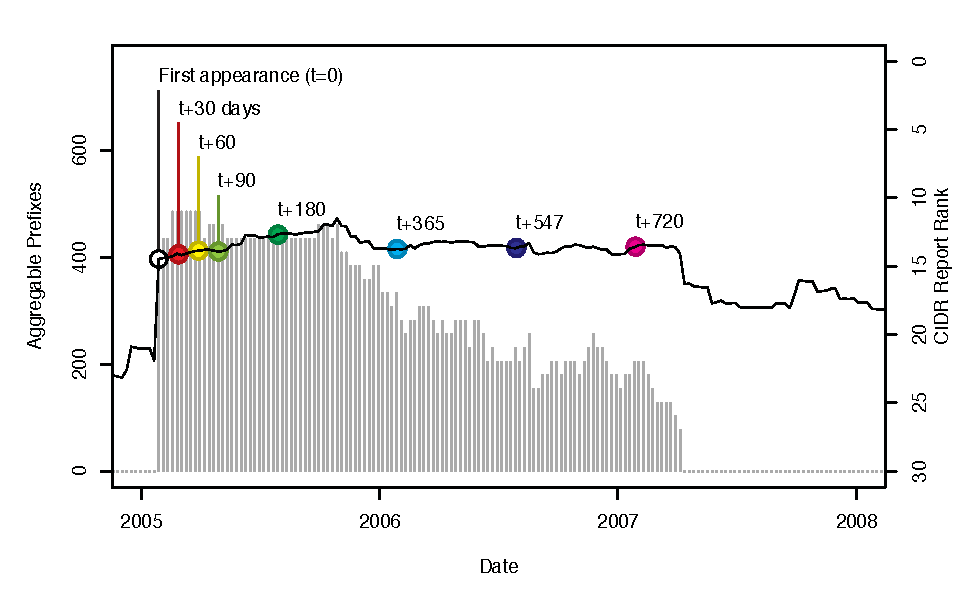
\includegraphics[width=6in]{figures/single_as.pdf}
    \vspace{-2em}\\
    \caption[Illustration of the sampling approach used to measure AS behavior]{Illustration of the sampling approach used to measure AS behavior, showing the first appearance (shown by the vertical bars indicating ranking on the authoritative CIDR Report) and samples at various durations thereafter. In this case, aggregable prefixes (netgain) are sampled from AS 3602.}
    \label{fig:sample_ex}
\end{centering}
\end{figure}

With these samples collected, differences are then calculated for each of these quantities relative to the first appearance to understand the behavior change of the AS relative to its initial appearance. Visualizations and analyses of these differences and other composite measures created using them are presented in the next chapter.

\subsection{Establishing the control group}

The process above, explained in terms of the treatment group of ASes that appear on the authoritative CIDR Report, is identical for the control group, with the exception of identification of ``appearances'' for the control group, as the ASes that compose the control group never appear on the CIDR Report. Instead, appearances in the control group must be constructed. In attempt to avoid biased construction of the control group, the control group is constructed randomly as follows.

First, a candidate set of ASes that are elligible to form the control group is established based on the following elligibility criteria:
\begin{itemize}
\item{An AS must announce at least 10 prefixes into the routing table in order to be elligible. This is an arbitrary minimum threshold, but it is intended to exclude the large proportion of stub ASes in the routing table that announce single prefixes \cite{6447-table-report}. The implications of the selection of this threshold is discussed further in the validity section of the next chapter.}
\item{An AS must be continuously visible in the routing table for a minimum of 2 years (720 days) to enable full sampling of its behavior.}
\end{itemize}

From the set of candidate ASes matching this criteria, a number of ASes equal to the number of ASes appearing on the authoritiative CIDR Report are randomly selected to form the control group. Finally, for each AS within the control group, the date of first ``appearance'' is randomly selected between the AS' first appearance in the routing table and 720 days before it's last appearance in the routing table. With these appearances established, the sampling and difference calcluation for the control group proceeds as with the treatment group.

% Handling gaps in the data
%    continue them until the end of the gap
% Extract data from CIDR Report according to intitial selection criteria
% Define and determine appearances from CIDR Report data
%    **NOT** four weeks on the report -- whooops
%    maximum gap of 8 weeks -- avoid multiple appearances
%    also remove overlap by amalgamating appearances that start within two years of eachotehr
% Select control group candidates and establish ``appearances'' within the control group
%    minimum
% For both the treatment and control group, measure behavior at various time intervals out from the initial appearaance

%////////////////////////////////////////////////////////////////////////
\chapter{CIDR Report Characteristics \& Influence on AS Behavior}
\label{chap:analysis}

This chapter presents and describes observed characteristics of the CIDR Report,
as well as the results of the analysis conducted to determine if the CIDR Report
affects network operator route aggregation behavior. The chapter begins with
a preliminary discussion about the availability of data and the quality of our
aggregation report implementation. This is followed by presentation of
characteristics of the CIDR report that were observed during this analysis and
will be discussed in the following chapter as clues of what may have affected
the success of the CIDR Report. The chapter concludes with presentation of the
main results of the analysis relevant to this thesis, illustrating how
individual AS' route announcement behavior may have been affected by appearing
on the CIDR Report. Finally, potential questions about the validity of the
analysis are identified and discussed.

As discussed briefly in the previous chapter, there are two data sets at play in
this analysis. The distinction between these two sets is important for
understanding some of the figures in this section, and so they are clearly
defined here:
\begin{itemize}
\item{\textbf{The Authoritative CIDR Report (ACR):} This is the data from the
``authoritative'' CIDR Report that was emailed out to network operators that
identifies the 30 most deaggregated ASes. This is the set of ASes that would be
expected to display a treatment effect if the CIDR Report was influential.}
\item{\textbf{The Generated CIDR Report (GCR):} This is the full aggregation
report generated by our implementation of the prefix aggregation algorithm used
by the CIDR Report, but containing data for every AS in the routing table
instead of being truncated after the 30th AS.}
\end{itemize}

Finally, to refresh the reader, some terms of art will be used in the remainder
of the chapter for conciseness. These are:
\begin{itemize}
\item{\textbf{netgain:} The number of prefixes advertised by an AS that are
unnecessary (do not affect routing policy from the perspective of the CIDR
Report vantage point), and could be removed from the routing table if this AS
aggregated perfectly.}
\item{\textbf{netsnow:} The total number of prefixes advertised by an AS,
including both aggregable and non-aggregable routes.}
\end{itemize}

\section{Addressing analytical quality/validity}

\subsection{Data availability}
Peculiarities and the historic origins of the underlying data sources for the
ACR and GCR mean that the data series for two reports start at different dates
and contain small gaps in their otherwise-continuous record of weekly CIDR
Report data. The start dates and gaps are illustrated in Figure
\ref{fig:avail_data}, where a solid vertical line indicates a week of available
data.

\begin{figure}[h!]
\begin{centering}
\begin{singlespace}
    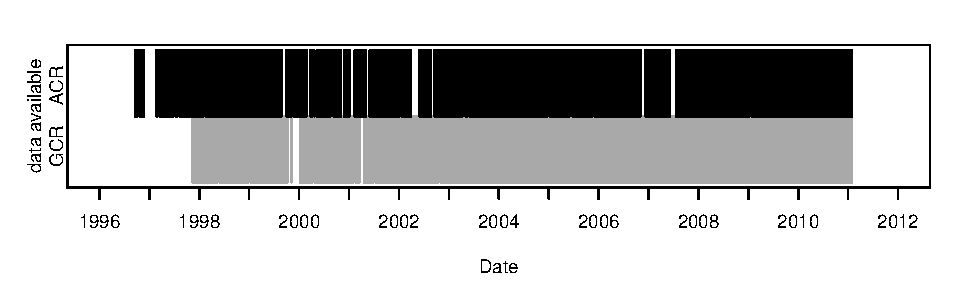
\includegraphics[width=6in]{figures/data_avail.pdf}
    \vspace{-2em}\\
    \caption{Available data}
    \label{fig:avail_data}
\end{singlespace}
\end{centering}
\end{figure}

As illustrated, data from both reports is generally available from November 1997
until January 2011, with a few relatively minor gaps. The period where the ACR
and GCR data overlap is the period used to analyze the effects of the CIDR
Report on AS behavior.

%	- plot total prefixes in the total table (Routeviews) and in the report (CIDR Report) to see that there aren't any discontinuities
% this is the "peer count" that I allude to

\subsection{GCR implementation quality}

In addition to data availability, the accuracy of the analysis that follows also
depends on the accuracy of our implementation of the CIDR Report aggregation
algorithm described in Chapter \ref{chap:method}. Recall that while the ACR is
used to determine when an AS appears on the CIDR Report (and thus potentially
commands attention of the community), the GCR is used to determine actual
post-appearance behavior because it provides consistently-generated measures
(like the number of aggregable prefixes advertised, \emph{netgain}) for ASes
both above and below the ACR top 30 threshold.

The first measure of accuracy is a comparison of the aggregable and total
prefixes determined for each AS on the ACR and GCR. A plot illustrating this
comparison is shown in Figure \ref{fig:comp_prefix_error}. The curves above the
horizontal zero ($y=0$) represent the sum of the differences in prefix counts
between the ACR and GCR for ASes where the GCR reports more prefixes than the
ACR. Similarly, the curves below the zero represent the sum of differences in
prefix counts between the ACR and GCR for ASes where the ACR reports more
prefixes than the GCR. The total deviation between the ACR and GCR is
given by the difference between the curves above and below zero.

\begin{figure}[h!]
\begin{centering}
\begin{singlespace}
    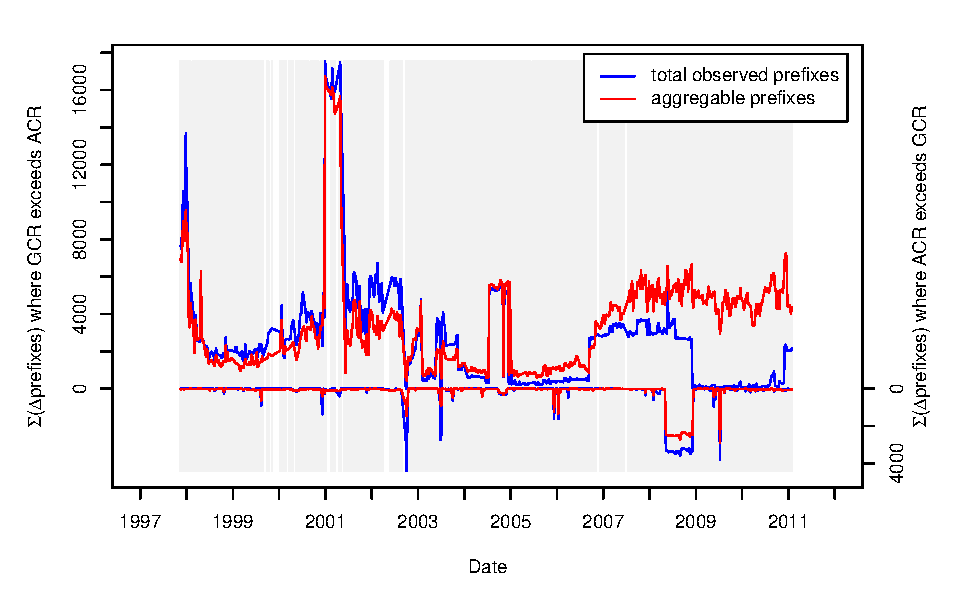
\includegraphics[width=6in]{figures/cidr_report_validity_prefix_error.pdf}
    \vspace{-2em}\\
    \caption{Differences in prefix counts between authoritative (ACR) and
        generated (GCR) CIDR Reports over time.}
    \label{fig:comp_prefix_error}
\end{singlespace}
\end{centering}
\end{figure}

As can be seen in Figure \ref{fig:comp_prefix_error}, throughout the period of
available data, the GCR generally claims larger quantities of aggregable and
total prefixes than the ACR. This is particularly pronounced and erratic when
compared against the pre-August 2002 CIDR Report (the point when the report's
methodology was changed when it was re-implemented by Geoff Huston). It is
difficult to determine the cause of this, but we suspect it is due to the
greater number of vantage points used in generating the GCR, leaving the GCR
more open to observing prefixes not visible from the ACR vantage point, or
observing AS\_PATHs that enable classification of prefixes as aggregable.

After August 2002, agreement between the ACR and GCR improves, though there are
still inconsistencies. Most of these inconsistencies appear attributable to
the GCR observing more prefixes than the ACR---this is the case when the
observed prefixes (blue line) and aggregable prefixes (red line) increase
simultaneously. Perhaps more concerning in terms of accuracy is the change in
behavior that began in late 2008 and continues to the latest, where the ACR and
GCR observe the same number of prefixes (blue line is approximately zero) but
the GCR classifies 4000-5000 more prefixes as aggregable.
\fbox{TODO: insert note from notebook from when I looked into this}

In spite of these inconsistencies, which are generally minor in terms of
ACR-GCR disparity for individual ASes, the GCR presents a view of potential
routing table aggregability that is sufficiently consistent with the ACR to
enable our use of the GCR as a data source for analyzing individual AS
aggregation behavior after appearing on the CIDR Report. Further, the
principles by which the GCR classifies prefixes as aggregable, as described in
the previous chapter, appear to be reasonable and sound from a technical
perspective. Finally, as will be discussed next, these minor differences in
prefix counts do not greatly affect the ranks of ASes on the GCR when compared
to the ACR.

While it is helpful to look at differences in prefix counts, as this is the
major purpose for which the GCR is used (rather than the ranking it generates),
we can also compare the rankings it generates against the rankings from the ACR
to compare the relative accuracy of the GCR. Ranks provided by the GCR are not
currently used in this analysis, so I only briefly raise this before continuing
on.

Figure \ref{fig:comp_rank_error} illustrates the minimum and maximum absolute
differences between the ranks of ASes appearing on the ACR and the ranks of
corresponding ASes on the GCR.

\begin{figure}[h!]
\begin{centering}
\begin{singlespace}
    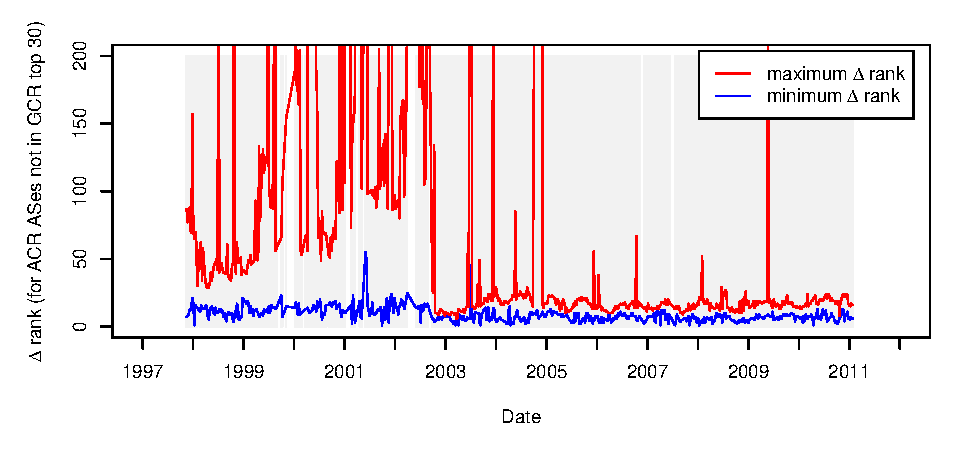
\includegraphics[width=6in]{figures/cidr_report_validity_rank_error.pdf}
    \vspace{-2em}\\
    \caption{Minimum and maximum differences in ASes ranked in the top 30 on
        the ACR but not in the top 30 on the GCR.}
    \label{fig:comp_rank_error}
\end{singlespace}
\end{centering}
\end{figure}

As can be seen, similar to the differences in prefix counts shown in the
previous figure, the rank differences are more significant and erratic from
1997 until August 2002, at which point they become more consistent. With some
exceptions, likely due to input data aberrations, the rankings generally differ
only a small amount, often near zero in the best case and no more than 20-30
in the worst case. Also, typically 20-25 of the ASes that appear on the ACR
also appear on the GCR (this is shown in a figure I may throw in the appendix).

% Figure \ref{fig:comp_top30_error} illustrates the total number of ASes ranked
% in the top 30 of the ACR that are not also in the top 30 of the GCR, as well as
% the rank of the first AS on the ACR not in the top 30 of the GCR.
%
% \begin{figure}[H]
% \begin{centering}
% \begin{singlespace}
%     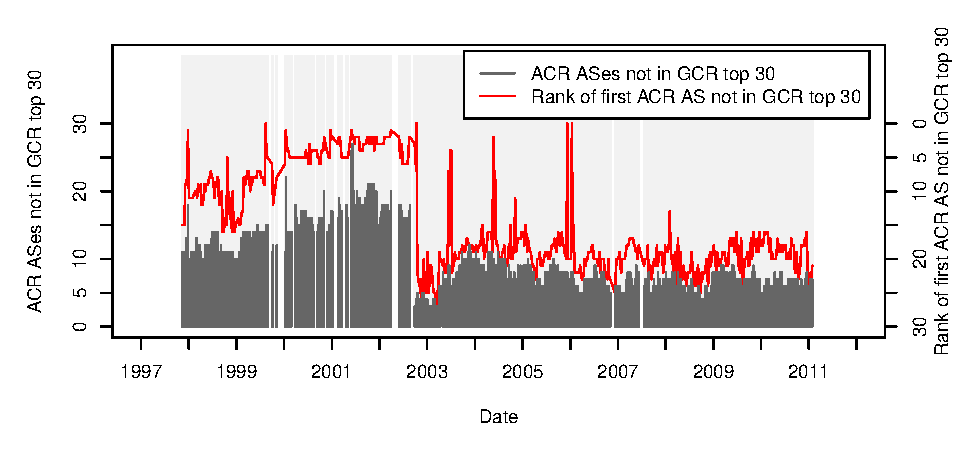
\includegraphics[width=6in]{figures/cidr_report_validity_top30_error.pdf}
%     \vspace{-2em}\\
%     \caption{The number and first rank of ASes in the treatment group (top 30)
%         of the ACR that are not in the treatment group of the GCR over time.}
%     \label{fig:comp_top30_error}
% \end{singlespace}
% \end{centering}
% \end{figure}

It was difficult to develop an implementation of the CIDR Report aggregation
algorithm (which is used to produce the GCR) that exactly matches the output of
the authoritative CIDR Report. Further, it is questionable whether an
implementation of the algorithm should strive to reproduce the output of a
``black box'' (even if it is the black box that is used to inform and influence
the operator community) instead of being based on first principles and a
conceptual understanding of the purpose of the CIDR Report. For these reasons,
along with the fact that the GCR is reasonably in agreement with the ACR, we
believe it is reasonable to use this data in our analysis.

\section{Characteristics of the CIDR Report}
In analyzing the CIDR Report, much time was spent looking at characteristics of
the report and networks that appear on it. While this was not directly related
to answering the question of whether appearing on the CIDR Report changes route
aggregation behavior, it is useful in providing context about the CIDR Report,
and also possibly offering insights about the causes of the behavior changes
that are observed in answering the question of this thesis. The characteristics
discussed in this section are organized into two categories: relative measures
of network behavior on the CIDR Report (typically related to ranks and ranking)
and absolute measures of network behavior (typically related to prefixes
advertised).

\subsection{AS Appearances and rank-based observations}
The first approach taken to gain an understanding of the behavior of the CIDR
Report was to visualize it in a two-dimensional space, with time in one
dimension and CIDR Report rank in the other dimension. An excerpt of this
visualization is shown in Figure \ref{fig:viz_sample}.

\begin{figure}[h!]
\begin{centering}
\begin{singlespace}
    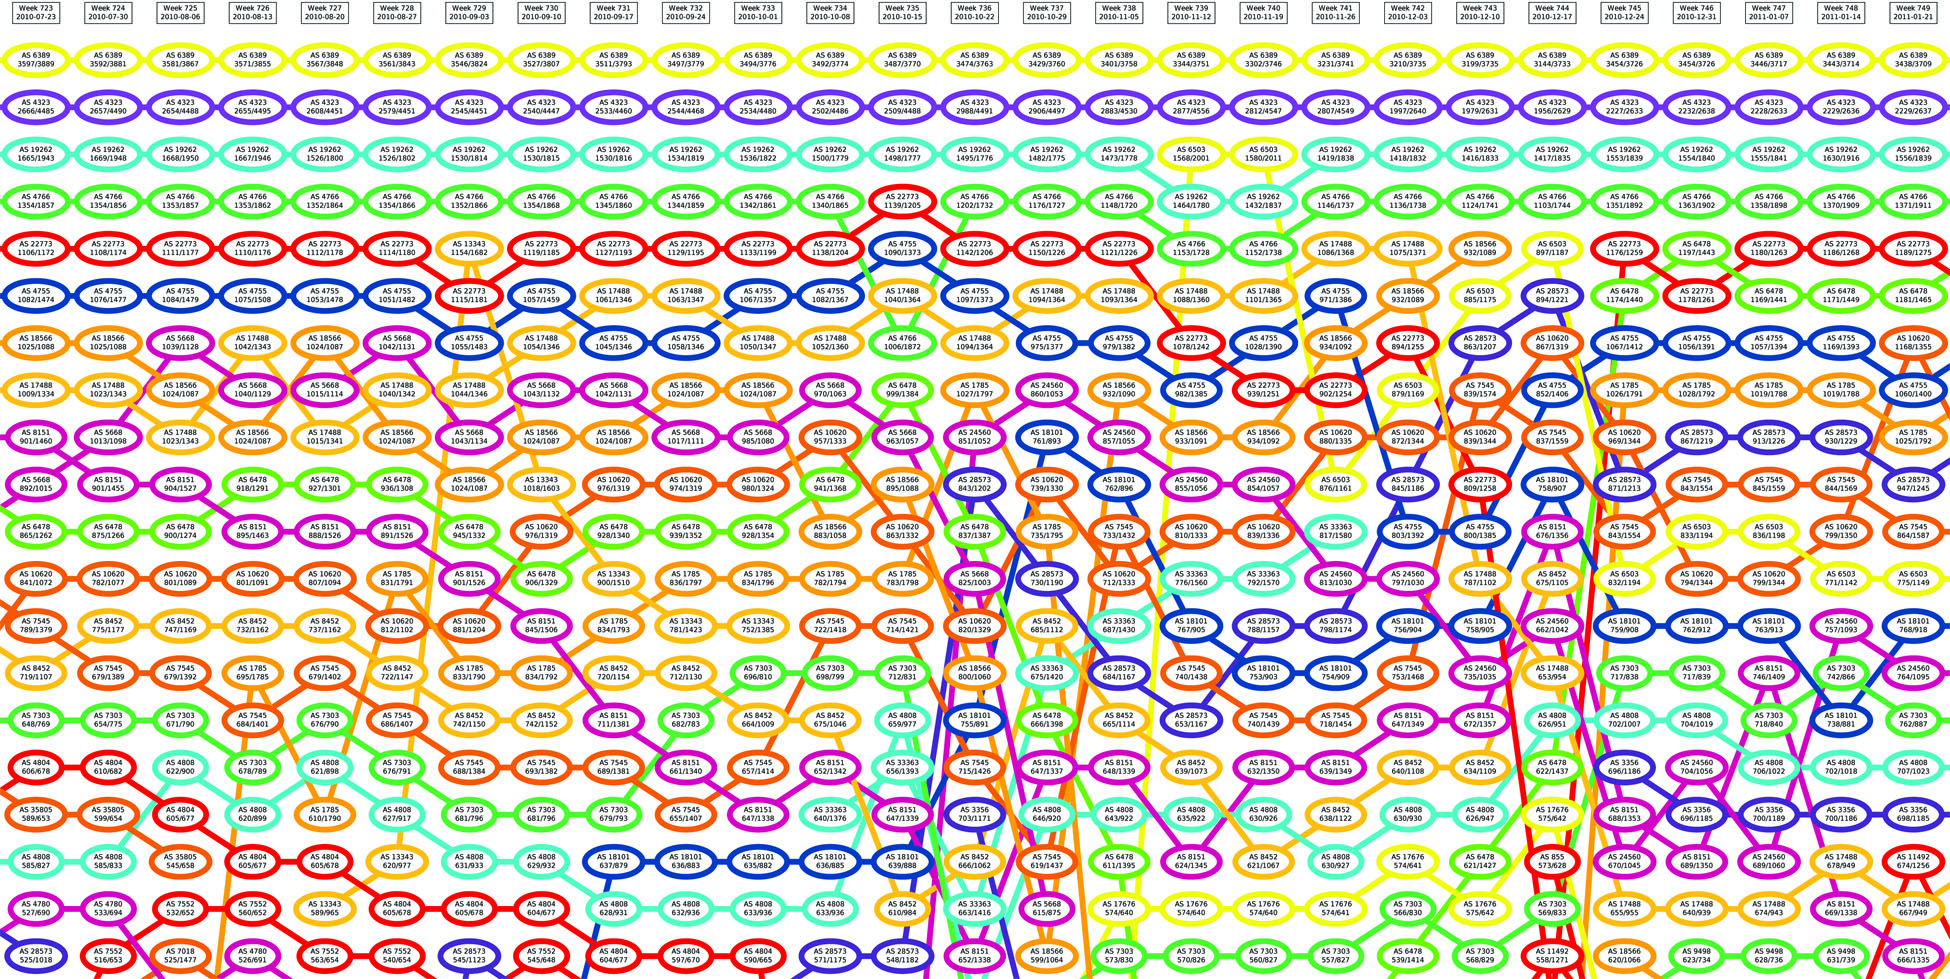
\includegraphics[width=4in]{figures/viz_sample.jpg}
    \caption{Visualization sample.}
    \label{fig:viz_sample}
\end{singlespace}
\end{centering}
\end{figure}

This visualization was not especially practical, as it was physically large and
the level of detail and limited range of colors available made it difficult to
visually identify and distinguish the behaviors of individual ASes. However,
this visualization provided some clues about interesting characteristics to
investigate. By visual inspection, it appeared as though the CIDR Report was
volatile at lower ranks but relatively static near the top (most aggregation
potential). It also appeared that the report was more volatile in the past but
become more static overall more recently. These and other aspects were then
investigated using analytic techniques, which are described and presented next.

A number of interesting characteristics about the CIDR Report are of a
demographic nature, such as how many ASes appear on the CIDR report, or for how
long do ASes remain on the report? This first question, about how many ASes
ever appear on the CIDR Report, is illuminated by Figure \ref{fig:as_counts}.

\begin{figure}[h!]
\begin{centering}
\begin{singlespace}
    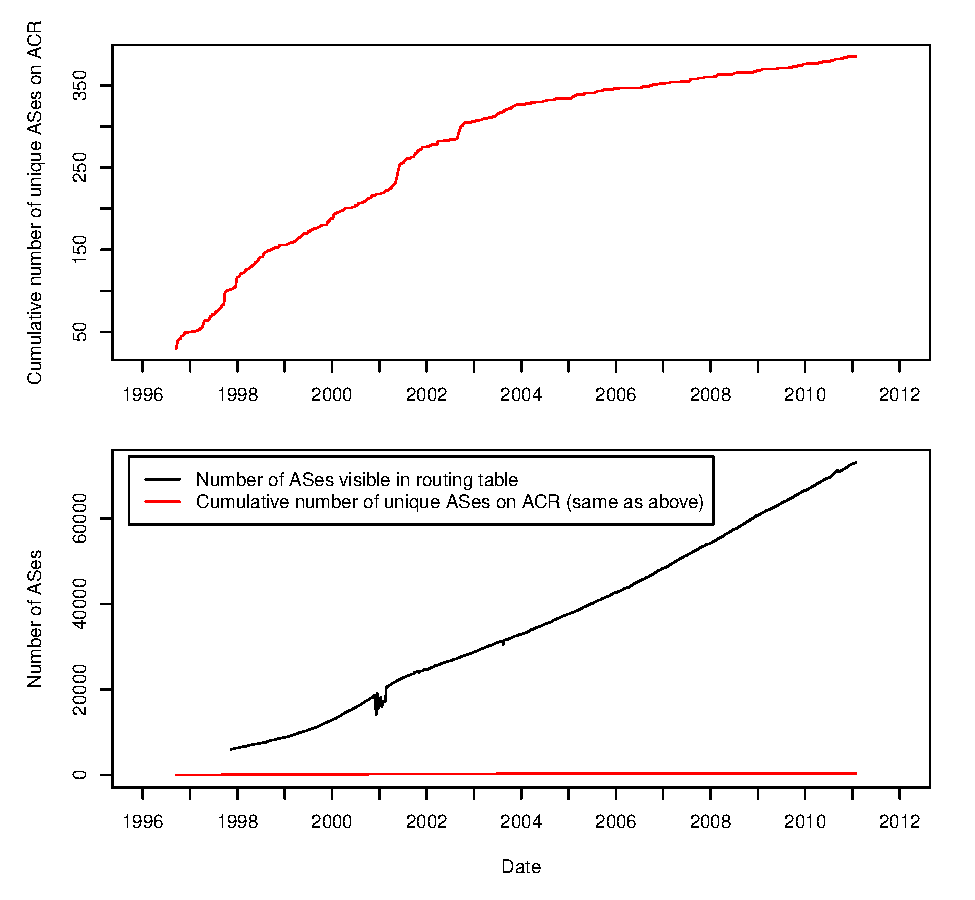
\includegraphics[width=6in]{figures/cumulative_asn_counts.pdf}
    \vspace{-2em}\\
    \caption{A cumulative count of the unique ASes that have appeared on the
        CIDR Report and compared to the cumulative count of unique ASes visible
        in the routing table up to the same point.}
    \label{fig:as_counts}
    %TODO: in future, think about plotting unique ASes ever appearing within
    %certain rank slots.
\end{singlespace}
\end{centering}
\end{figure}

In this figure, the top plot shows the cumulative number of ASes that appear on
the CIDR Report, starting with 30 ASes on the first report in 1996 and
concluding with 386 unique ASes in 2011. The growth of new ASes appearing on
the report appears to be greater in the late 1990s and early 2000s than in the
mid-late 2000s. More remarkable is how relatively few ASes from the total set
of ASes that ever appear in the Internet routing table appear on the CIDR
Report. This relationship is shown in the bottom plot of Figure
\ref{fig:as_counts}. In this figure, the red curve near the bottom of the graph
area is the same red curve that was plotted in the upper figure, and the black
curve that rises steadily is the total number of ASes visible in the routing
table. This illustrates that less than 1\% of all ASes have ever appeared on
the CIDR Report.

While the former plot illustrated the total number of ASes that appear on the
report, it does not provide any information about how long an AS appears on the
report for. This information is provided in the next figure. Figure
\ref{fig:cdf_weeks}, which presents a cumulative distribution function of the
total number of weeks each AS appears on the CIDR Report. Noting the log scale
on the x-axis, we can see that 15\% of all ASes that appear on the CIDR Report
are on the report for only a single week, half of all ASes are on the report
for approximately 10 weeks or less, and that there is a general exponential
relationship between increasing fractions of the population and time spent
on the report (i.e. for each 10\% increase in population considered, the
maximum duration spent on the report doubles).

\begin{figure}[h!]
\begin{centering}
\begin{singlespace}
    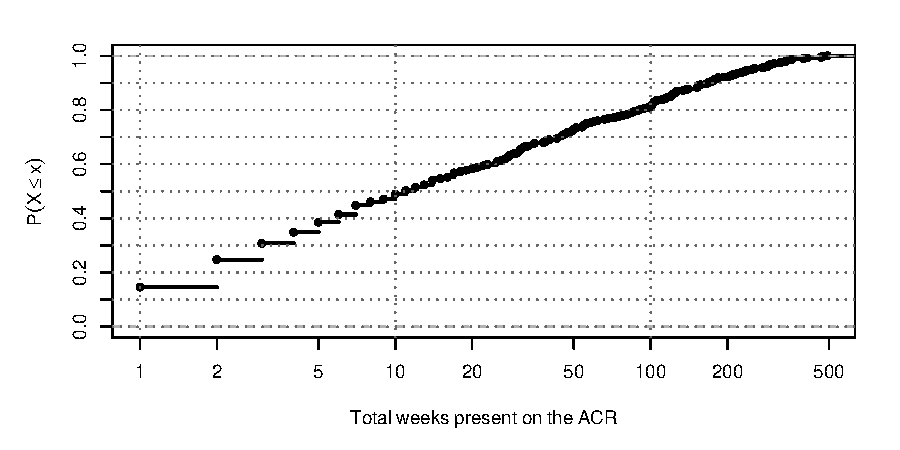
\includegraphics[width=6in]{figures/acr_cdf_weeks.pdf}
    \vspace{-2em}\\
    \caption{A cumulative distribution function of the total number of weeks
        that each AS is visible on the CIDR Report.}
    \label{fig:cdf_weeks}
\end{singlespace}
\end{centering}
\end{figure}

%TODO: tempting to take the following graf and figure out.
% A similar plot with a different metric is shown in Figure
% \ref{fig:cdf_rankweeks}. In this figure, instead of presenting the number of
% weeks each AS spends on the report, the number of rank-weeks accrued by each AS
% are displayed instead. A rank week is simply the sum of the ranks an AS
% occupies for each week it appears on the CIDR Report. So an AS could accumulate
% a rank-week measure of 100 by spending 100 weeks at the very bottom of the
% report (rank of 1, 30th position) or 10 weeks at a rank of 10 (20th position).
%
% \begin{figure}[h!]
% \begin{centering}
% \begin{singlespace}
%     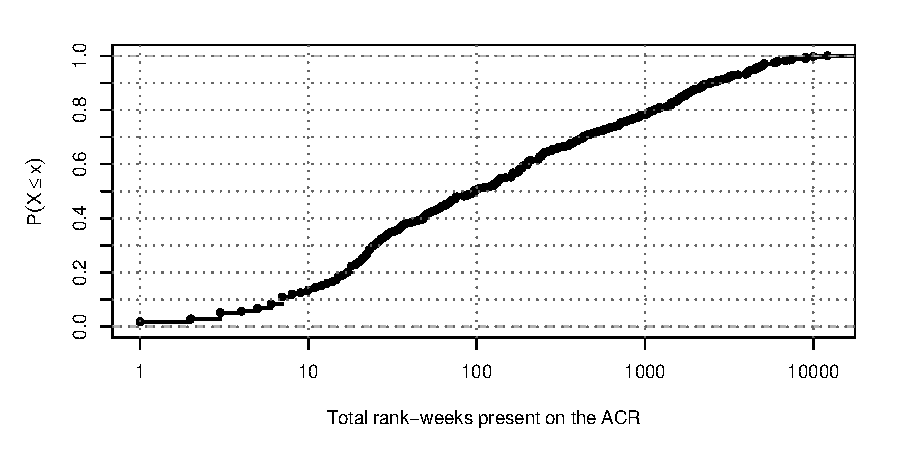
\includegraphics[width=6in]{figures/acr_cdf_rankweeks.pdf}
%     \vspace{-2em}\\
%     \caption{A cumulative distribution function of the total number of
%         rank-weeks that each AS is visible on the CIDR Report.}
%     \label{fig:cdf_rankweeks}
% \end{singlespace}
% \end{centering}
% \end{figure}

This is the first indication that not all the ASes that appear on the CIDR
report behave in similar ways, but instead that many ASes appear only briefly
in comparison to some ASes that occupy a considerable part of the CIDR Report.

% \begin{figure}[H]
% \begin{centering}
% \begin{singlespace}
%     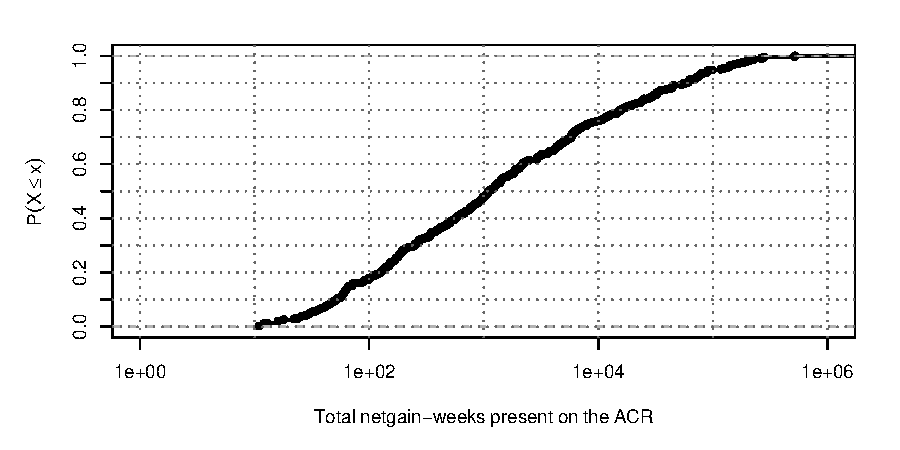
\includegraphics[width=6in]{figures/acr_cdf_ngweeks.pdf}
%     \vspace{-2em}\\
%     \caption{A cumulative distribution function of the total number of netgain-weeks that each AS is visible on the CIDR Report.}
% \end{singlespace}
% \end{centering}
% \end{figure}

Returning to the observation from earlier that the top ranks of the CIDR Report
are static relative to the volatile lower ranks, we investigated this further
by plotting cumulative distribution functions of the number of weeks that a
particular AS occupies a given rank on the CIDR Report. These plots, for ranks
1 (most potential for aggregation) to 30, are shown in groups in Figure
\ref{fig:rank_cdfs}

\begin{figure}[h!]
\begin{centering}
\begin{singlespace}
    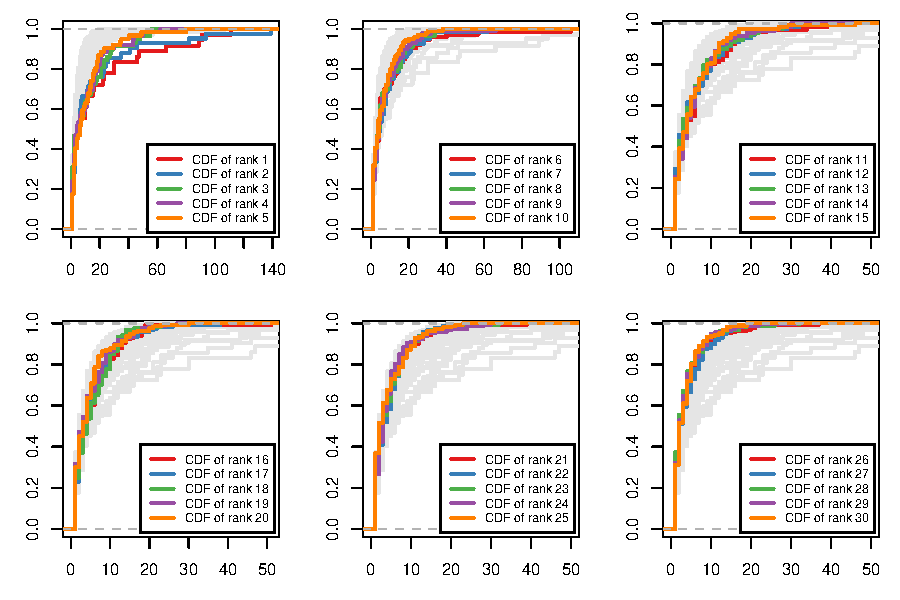
\includegraphics[width=6in]{figures/cr_rank_cdfs.pdf}
    \vspace{-2em}\\
    \caption{CDFs of the number of weeks that a given rank was occupied by a
    single AS. The x-axis is the number of weeks, and the y-axis is the
    fraction of the population. The light gray lines indicate CDFs of other
    ranks, in order to place the highlighted ranks in context.}
    \label{fig:rank_cdfs}
\end{singlespace}
\end{centering}
\end{figure}

As illustrated clearly by this figure, lower ranks on the CIDR Report are more
volatile than top ranks. The top five positions, ranks 1-5, are particularly
ossified, with the top 10\% of ASes that ever appear occupying individual ranks
for no less than 20-60 weeks. In contrast, the lower ranks, and particularly
the bottom half (ranks lower than 15) are much more volatile, with around
90\% of the AS population occupying a given rank for 10 weeks or less, and
essentially all of the population not occupying ranks for more than 20
weeks. This is consistent with the claimed observation of operators that
the CIDR Report does not appear to change much---especially the top ranks
that are first visible in the email. What appears to be the apparent reason
for this ossification will be discussed in the next section.

\subsection{Prefix-based observations}

%TODO: include a figure of the proportion of the routing table that is
%aggregable/deaggregated over time? Plot deagg_factor or frac_aggr?

While the previous section made some interesting observations about ASes'
appearance and movement behavior through the CIDR Report, it was focused on the
relative measures of AS rank (and relatedly, appearance within the top 30) on
the CIDR Report. It is also helpful to gain a perspective about characteristics
of the CIDR report considering the prefixes that each AS is advertising, as
prefix counts (and routing table slots) are ultimately the metric that is
important in considering behavior change in the context of the routing table.

Figure \ref{fig:netcompare}\footnote{All data in this plot is from the GCR, but
classification of an AS and its netgain/netsnow figures are based on the ASes
present on the ACR as emailed. Data from the GCR is used to allow for consistent
comparison between the entire routing table and the top 30 (ACR) ASes.}
illustrates what fraction of the the total prefixes and aggregable prefixes
visible in the Internet routing table are advertised by ASes appearing on the
CIDR Report.

\begin{figure}[h!]
\begin{centering}
\begin{singlespace}
    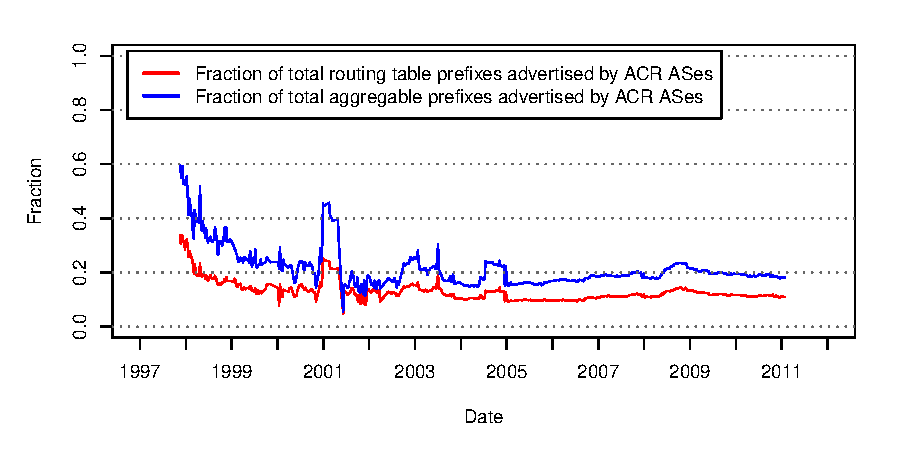
\includegraphics[width=6in]{figures/acr_gcr_netcompare2.pdf}
    \vspace{-2em}\\
    \caption{Plots of the fractions of total prefixes and total aggregable
    prefixes in the routing table that are advertised by ASes appearing on the
    CIDR Report.}
    \label{fig:netcompare}
\end{singlespace}
\end{centering}
\end{figure}

This figure suggests that in the past, the CIDR Report did indeed focus quite
effectively on the ``worst offenders'' in terms of networks advertising
aggregable routes---at the beginning of the period of available data, it
captured nearly 60\% of the total aggregable routes in the top 30 list. This
has dropped off and, interestingly, remained approximately proportional to the
growth of the routing table since 2003 or 2004, suggesting that growth of
deaggregation in the ASes at the top of the CIDR Report is proportional to the
growth of deaggregation across the Internet routing table. However, as the next
figure will show, this proportionality has been maintained in the face of
growth of the number of participants in the Internet routing table, such that
the ASes that appear at the top of the report have become disproportionally
deaggregated.

Another way of considering how the prefix advertisement behaviors of networks
on the CIDR Report relates to other networks in the routing table is to look at
the distribution of deaggregation (advertisement of aggregable prefixes) in the
routing table. Cumulative distribution functions of aggregable prefixes
(netgain) visible in the routing table (from the GCR) over time is shown in
Figure \ref{fig:netgain_cdf}.

% TODO in future, look into whether the distribution of deaggregators is a
% power-law relationship
\begin{figure}[h!]
\begin{centering}
\begin{singlespace}
    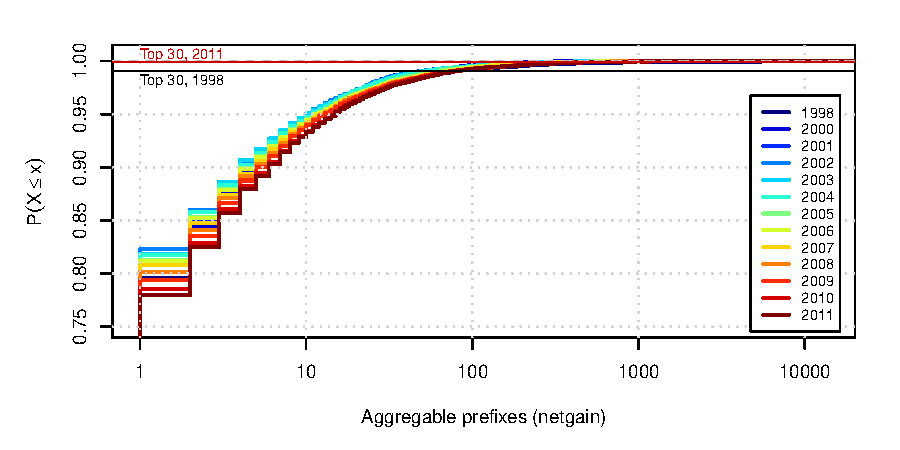
\includegraphics[width=6in]{figures/netgain_cdf_gcr.pdf}
    \vspace{-2em}\\
    \caption{CDFs of netgain of all ASes in the routing table in the first week
    of the year from 1998-2011. Threshold lines indicating the cutoff point for
    appearing on the CIDR Report in 1998 and 2011 are indicated. Note that the
    graph is rescaled; approximately 70\% of ASes in the routing table do not
    advertise any aggregable prefixes.}
    \label{fig:netgain_cdf}
\end{singlespace}
\end{centering}
\end{figure}

From these distributions we can see that while advertisement of aggregable
prefixes has increased slightly across the routing table over time, as given by
the downward move in the CDF curves over time, the distribution of aggregable
prefixes announced by ASes has remained roughly similar, with an increasingly
long long-tail of outliers in the top fraction of a percentile of the
population of ASes. This figure is potentially misleading, as while the
distribution of aggregable prefix announcement has not changed, the total
number of ASes visible in the routing table has grown over time, from 3172 ASes
in the first week of 1998 to 36383 ASes in the first week of 2011. Thus, there
are approximately ten times the number of ASes announcing the same number of
aggregable prefixes now than in 1998.

What is also noteworthy in this figure is the indication of
the threshold points for appearing on the CIDR Report in 1998 and 2011. The
fraction of the population above this line is the ``top 30'' group that would
appear on the CIDR Report. This line appears to have moved from approximately
1\% of the population to some small fraction of a percent. This conclusion
follows from the fact that the number of ASes in the routing table has grown
over time and yet the length of the CIDR report has remained the same. However,
as this figure, as well as Figure \ref{fig:netcompare} illustrate, this also
means that the CIDR Report has changed to highlight mostly outlier behavior,
leaving the individually less significant but collectively more significant
deaggregation below the threshold unaddressed.

% \begin{figure}[H]
% \begin{centering}
% \begin{singlespace}
%     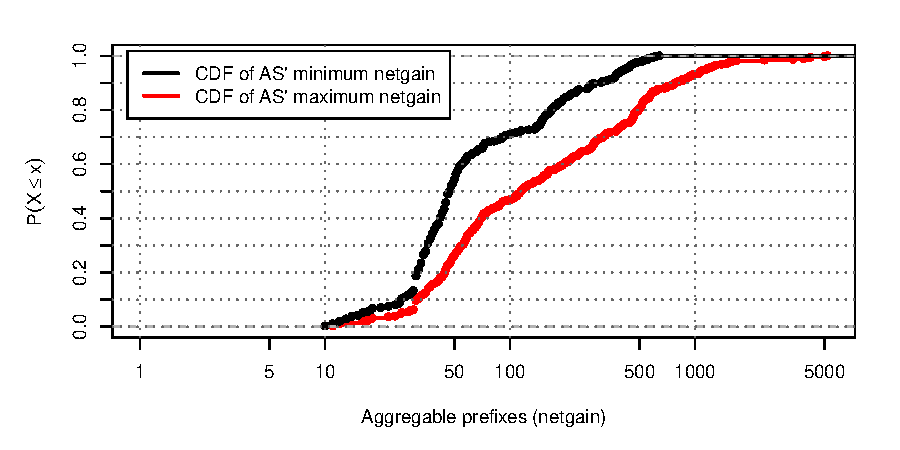
\includegraphics[width=6in]{figures/acr_netgain_cdfs.pdf}
%     \vspace{-2em}\\
%     \caption{CDFs of the minimum and maximum netgain observed for each AS during its time on the CIDR Report.}
% \end{singlespace}
% \end{centering}
% \end{figure}

The question of where the threshold to appear on the CIDR Report is---how much
deaggregation it takes for an AS to appear on the report---is addressed in
Figure \ref{fig:thresholds}. This figure displays the minimum netgain
thresholds to appear on the CIDR Report (rank 30) as well as the median (rank
15) and various other top ranks.

\begin{figure}[h!]
\begin{centering}
\begin{singlespace}
    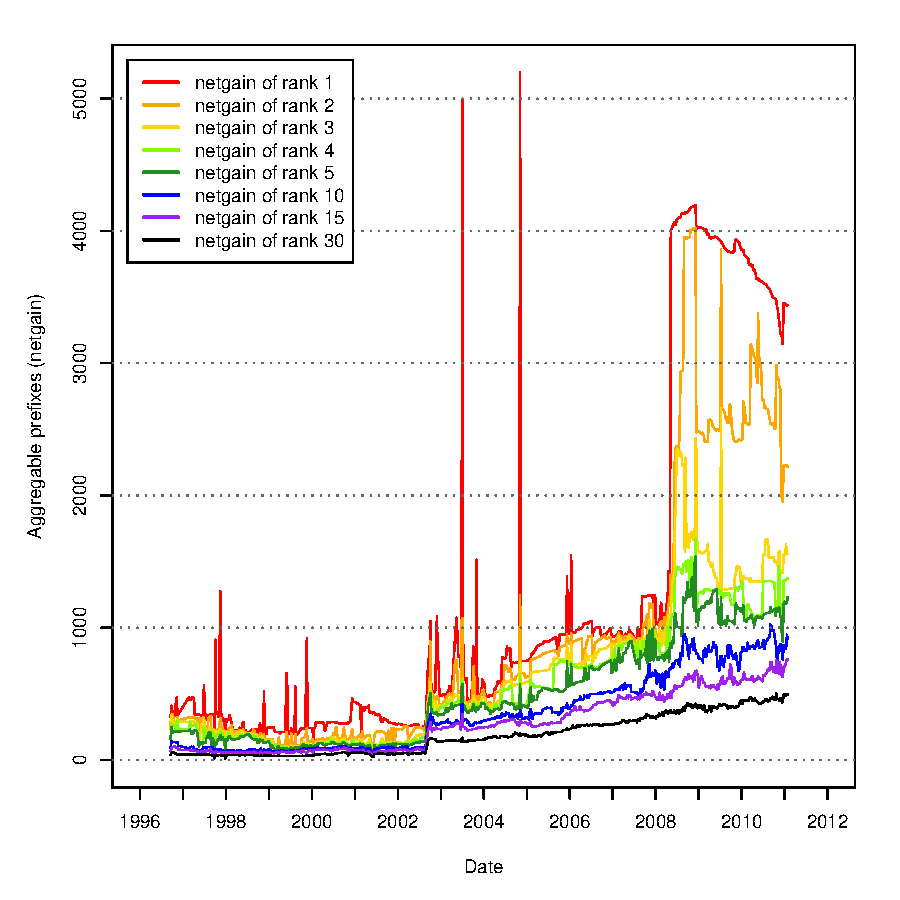
\includegraphics[width=6in]{figures/acr_netgain_time.pdf}
    \vspace{-2em}\\
    \caption{The netgain thresholds required to achieve indicated ranks on the
    ACR over time.}
    \label{fig:thresholds}
    \end{singlespace}
\end{centering}
\end{figure}

This figure of the CIDR Report rank thresholds shows an increasing spread in
prefix thresholds for the various ranks over time, particularly in the top 5,
as well as between the top 5 and the median, compared to between the median and
the minimum threshold (rank 30). The increasing spread between ranks can also
be viewed in a slightly different way, with a focus on temporal progression, in
the following figure. Figure \ref{fig:netgain_cdf_acr} presents cumulative
distribution functions of the number of aggregable prefixes (netgain)
advertised by each AS on the ACR in the first week of the year indicated.

\begin{figure}[h!]
\begin{centering}
\begin{singlespace}
    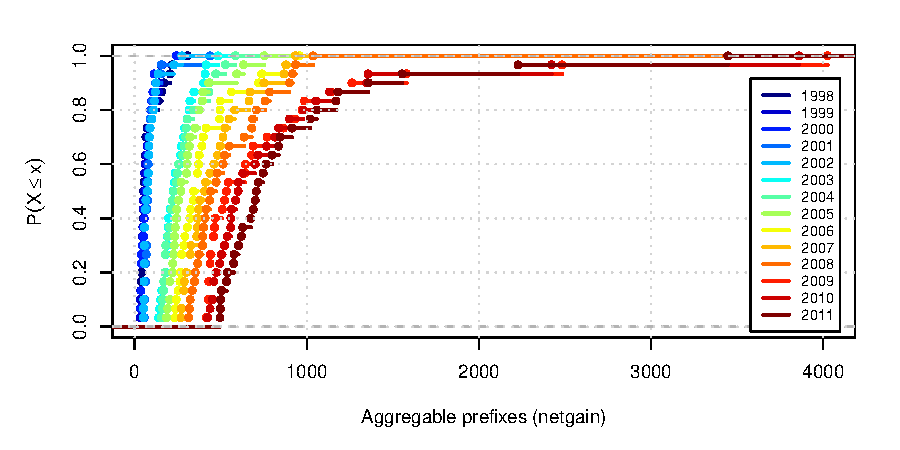
\includegraphics[width=6in]{figures/netgain_cdf_acr.pdf}
    \vspace{-2em}\\
    \caption{Plots of CDFs of the netgain of the ASes visible on the ACR in the
    first week of each year 1998-2011. Notice that the top of the population
    spreads more in later years.}
    \label{fig:netgain_cdf_acr}
\end{singlespace}
\end{centering}
\end{figure}

Here again we see the growing spread between ranks and the changing shape of
the distribution as ASes at the top of the report differ from the bottom more
in later years than in previous years. Both this and the previous plot suggest
that the ossification in the top ranks of the CIDR report observed earlier are
due to the growing spread in netgain, making it more difficult to ``unseat''
high-ranked ASes because they are so far from the next nearest AS (in terms of
number of prefixes). This is not necessary a problem, and also our measure of
volatility may be imperfect (i.e. an AS could oscillate between two ranks,
appearing volatile even though its behavior does not chance perceptibly), but
this does provide some explanation for the static behavior noted before.

% Finally, just because it is interesting, I include a plot of the minimum
% threshold, in terms of aggregable prefixes, that are necessary to appear on the
% CIDR Report over time.
%
% %TODO should I include this???
% \begin{figure}[H]
% \begin{centering}
% \begin{singlespace}
%     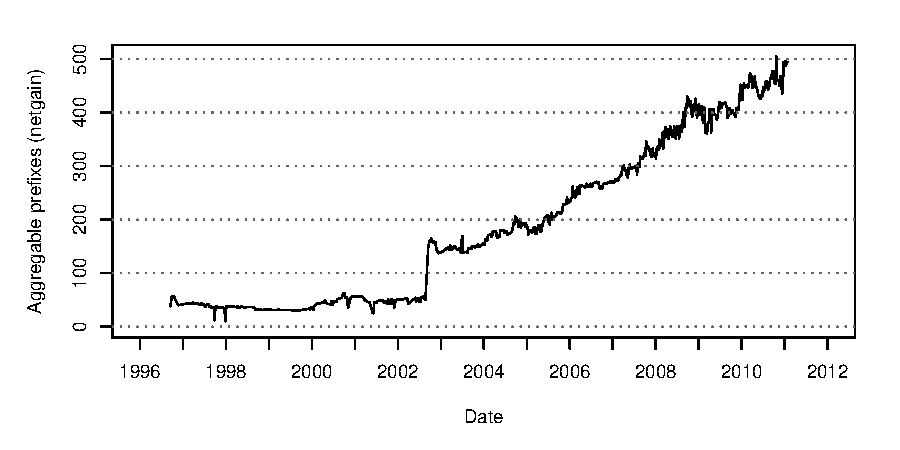
\includegraphics[width=6in]{figures/acr_netgain_time_min.pdf}
%     \vspace{-2em}\\
%     \caption{A plot of the minimum netgain required to appear on the CIDR
%     Report over time.}
%     \end{singlespace}
% \end{centering}
% \end{figure}

%TODO should I include this???
% \begin{figure}[h!]
% \begin{centering}
% \begin{singlespace}
%     \includegraphics[width=6in]{figures/netgain_frac_aggr_cdf_gcr.pdf}
%     \vspace{-2em}\\
%     \caption{Plots of CDFs of the fraction of prefixes announced by each AS
%     that are aggregable, over time.}
%     \label{fig:netgain_cdf_acr}
% \end{singlespace}
% \end{centering}
% \end{figure}

\subsection{Conclusions}

Both these observations of characteristics of the CIDR Report related to the
number of prefixes advertised by each AS, as well as the previous observations
about the rank of each AS and appearance of ASes on the CIDR Report, suggest
that while the advertisement of redundant, aggregable prefixes in the routing
table is reasonably commonplace, the ASes that appear on the CIDR Report are
outliers in that they announce significantly more aggregable prefixes than most
of the rest of the population of ASes participating in the interdomain routing
system. In its earlier days the CIDR Report captured a larger fraction of the
ASes responsible for aggregable prefixes than it does now, because of
growth in the number of ASes announcing aggregable routes, and the top of the
report seems to have become relatively static because of the extreme
deaggregation of ASes at the top of the report relative to the majority of the
AS population.

\section{Analysis of AS behavior after appearing on the CIDR Report}

This section presents and discusses the results of the primary question of this
thesis, \emph{do autonomous systems change their behavior, as measured by the
number of aggregable routes they advertise into the routing table (netgain),
after appearing on the CIDR Report?} As described in section
\ref{sec:method_agg_report_analysis}, data from the CIDR Report is processed to
determine when ASes first appear on the report, and samples are then take from
30 to 730 days after this initial appearance (detailed in Figure
\ref{fig:sample_ex}) and compared to the value at the time of first appearance.
Decreases in netgain would suggest that the CIDR Report does influence network
operator route aggregation behavior in the expected or intended way, while no
change or increased netgain would suggest that the CIDR Report has no effect.
The group of ASes appearing on the CIDR Report, and thus theoretically subject
to social forces to improve aggregation behavior, will hereafter be referred to
as the treatment group.

In an attempt to control for normal variation in AS behavior that does not
result from appearing on the CIDR Report, a ``control group'' was established
from ASes never appearing on the CIDR Report, as described in much more detail
in section \ref{sec:method_agg_report_analysis}, to determine the behavior of
ASes that are not treated by the CIDR Report. As this is a quasi-experiment
rather than a randomized, controlled experiment, this group will hereafter be
referred to as the ``untreated group'' instead.

A number of quantities are measured and presented in the following section, in
an effort to discern the behavior of ASes appearing on the CIDR Report. They
are as follows (in all cases, $t$ is symbolic of the time of first appearance,
and $k$ is one of the measurement time periods from 30-730 days):
\begin{itemize}
\item{Change in netgain: $\Delta\textrm{netgain}_{t+k} = \textrm{netgain}_{t+k}
    - \textrm{netgain}_{t+0}$}
\item{Relative change in netgain: $\frac{\Delta\textrm{netgain}_{t+k}}
    {\textrm{netgain}_{t+0}}$}
\item{Change in netsnow: $\Delta\textrm{netsnow}_{t+k} = \textrm{netgain}_{t+k}
    - \textrm{netsnow}_{t+0}$}
\item{Relative change in netsnow: $\frac{\Delta\textrm{netsnow}_{t+k}}
    {\textrm{netsnow}_{t+0}}$}
\item{Fraction of prefixes that are aggregable (``fraction aggregable''):
    $\frac{\textrm{netgain}_{t+k}} {\textrm{netsnow}_{t+k}}$}
% \item{Deaggregation factor: $\frac{\textrm{netsnow}_{t+k}}
%     {\textrm{netsnow}_{t+k} - \textrm{netgain}_{t+k}}$}
\end{itemize}

Note that the final quantity above, while a useful measure of deaggregation,
is not measured relative to the original appearance point, and so must be
viewed together with the fraction aggregable measure at the original point of
appearance ($t+0$) in order to observe change in behavior.

With this initial explanation, we are ready to present the results of our
analysis, beginning with netsnow and netgain, and followed with fraction
aggregable, which demonstrates the greatest observed behavior change. Unless
otherwise noted in captions of the figures or the associated text, all of the
following figures utilize all appearances on the CIDR Report from 1997-2011.
Figures of these quantities utilizing appearances from only a portion of the
date range, to discern changes in behavior over time, are included in Appendix
\ref{chap:additional_figs}.

\subsection{Change in netgain in response to CIDR Report appearance}

\begin{figure}[H]
\begin{centering}
\begin{singlespace}
    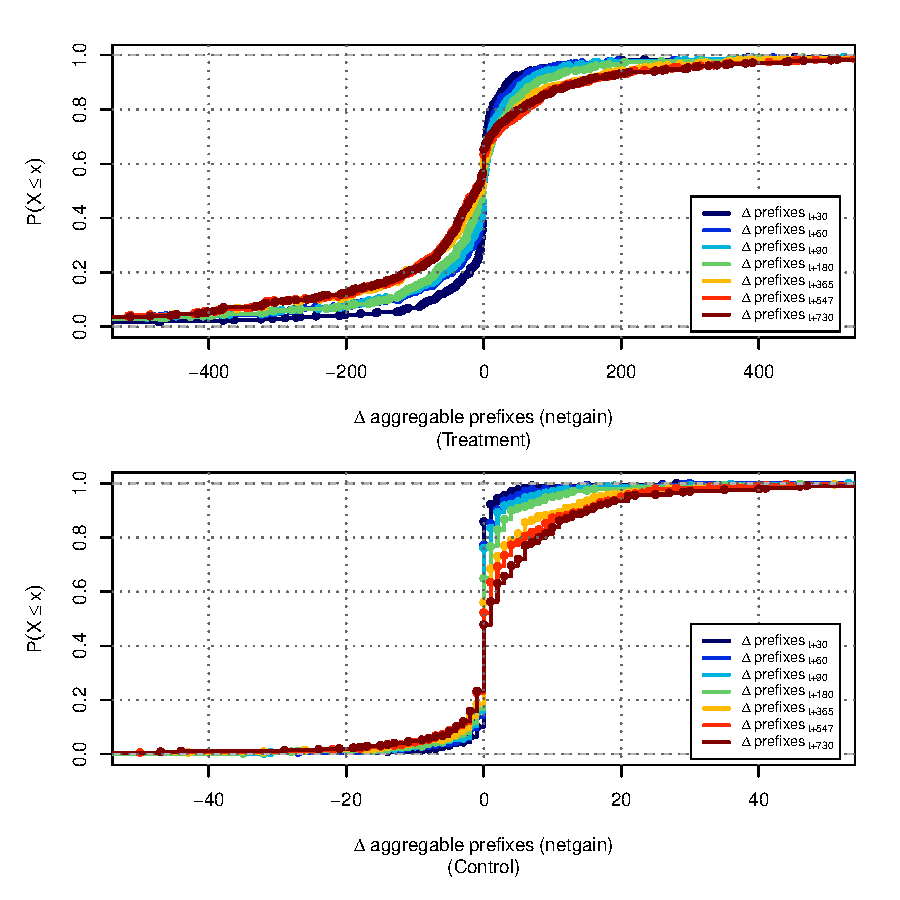
\includegraphics[width=6in]{figures/behavior-netgain-1997_2011-corr.pdf}
    \vspace{-2em}\\
    \caption{Cumulative distribution function of change in number of aggregable
    prefixes (netgain) advertised by treated and untreated (control) ASes, for
    the period 1997-2011.}
\end{singlespace}
\end{centering}
\end{figure}

\begin{figure}[H]
\begin{centering}
\begin{singlespace}
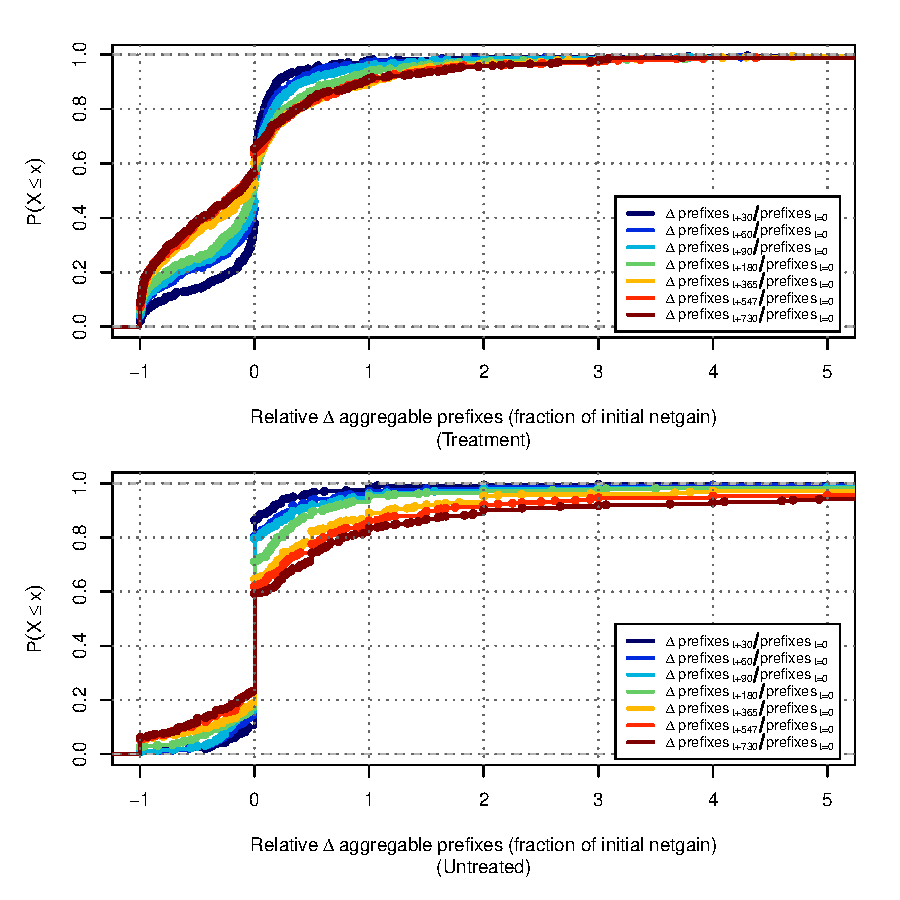
\includegraphics[width=6in]{figures/behavior-rel_netgain-1997_2011-corr.pdf}
    \vspace{-2em}\\
    \caption{Cumulative distribution function of relative change in number of
    aggregable prefixes (netgain) advertised by treated and untreated (control)
    ASes, for the period 1997-2011.}
\end{singlespace}
\end{centering}
\end{figure}

\subsection{Change in netsnow in response to CIDR Report appearance}

\begin{figure}[H]
\begin{centering}
\begin{singlespace}
    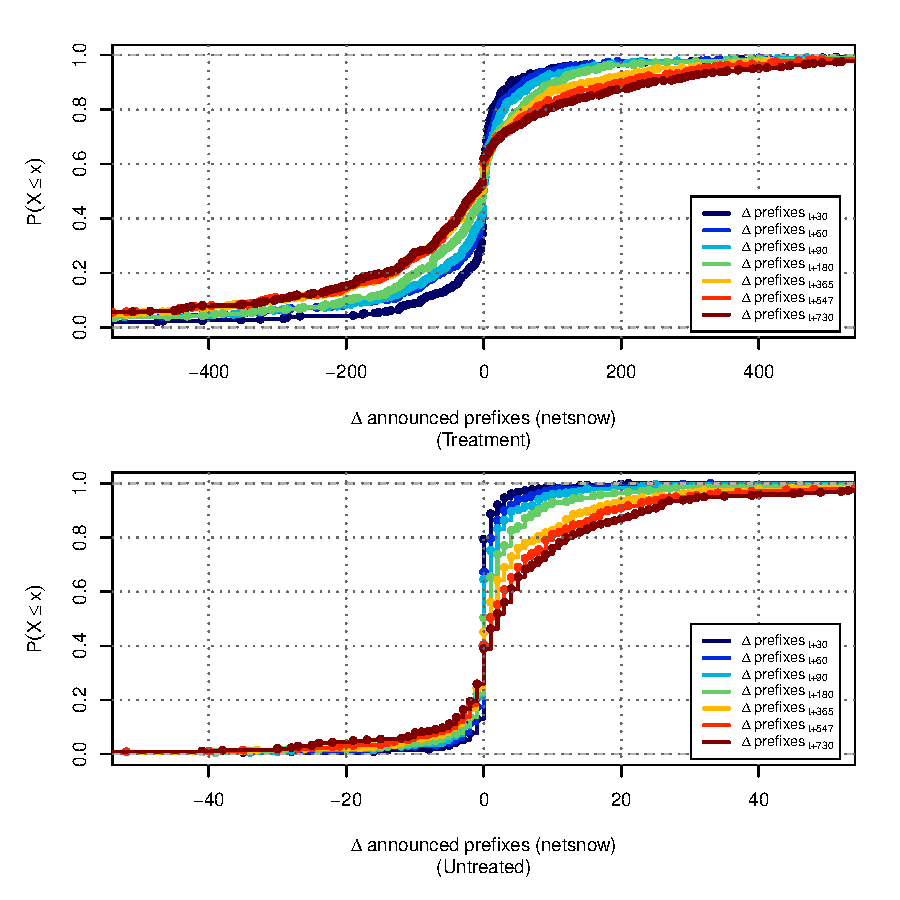
\includegraphics[width=6in]{figures/behavior-netsnow-1997_2011-corr.pdf}
    \vspace{-2em}\\
    \caption{Cumulative distribution function of change in total number of
    prefixes (netsnow) advertised by treated and untreated (control) ASes, for
    the period 1997-2011.}
\end{singlespace}
\end{centering}
\end{figure}

\begin{figure}[H]
\begin{centering}
\begin{singlespace}
    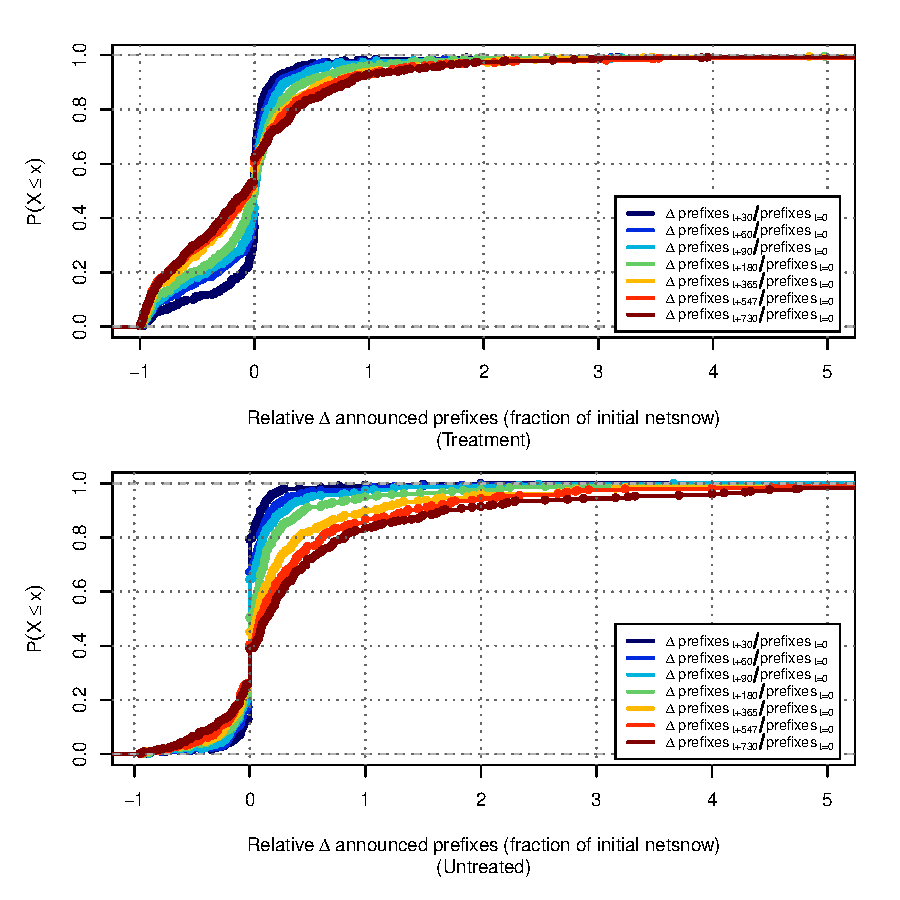
\includegraphics[width=6in]{figures/behavior-rel_netsnow-1997_2011-corr.pdf}
    \vspace{-2em}\\
    \caption{Cumulative distribution function of relative change in total
    number of prefixes (netsnow) advertised by treated and untreated (control)
    ASes, for the period 1997-2011.}
\end{singlespace}
\end{centering}
\end{figure}

\subsection{Change in fraction aggregable in response to CIDR Report appearance}

\begin{figure}[H]
\begin{centering}
\begin{singlespace}
    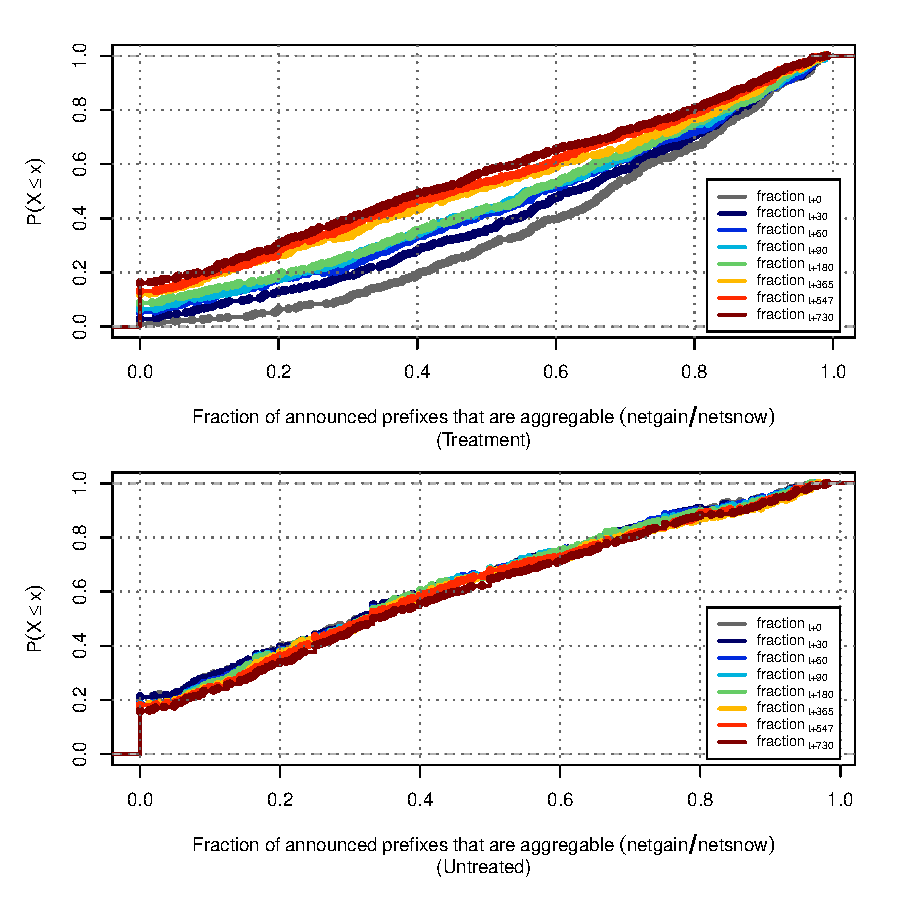
\includegraphics[width=6in]{figures/behavior-frac_deagg-1997_2011-corr.pdf}
    \vspace{-2em}\\
    \caption{Cumulative distribution function of change in the fraction of
    prefixes advertised by treated and untreated (control) ASes that can be
    aggregated without affecting routing policy, for the period 1997-2011.}
\end{singlespace}
\end{centering}
\end{figure}

\begin{figure}[H]
\begin{centering}
\begin{singlespace}
    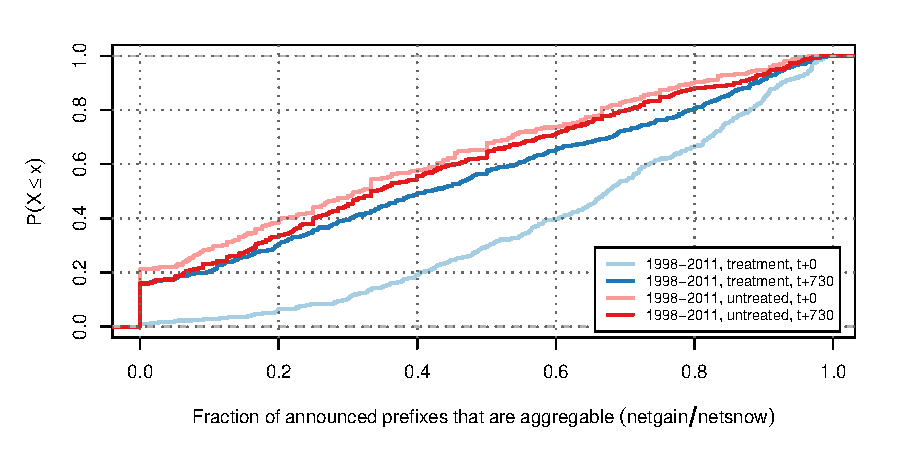
\includegraphics[width=6in]
        {figures/behavior-frac_deagg-1997_2011-special_tc.pdf}
    \vspace{-2em}\\
    \caption{Simplification of previous figure, showing the first (t+0) and
    last (t+730) CDF of the fraction aggregable for both the treatment and
    untreated groups.}
\end{singlespace}
\end{centering}
\end{figure}





\begin{figure}[H]
\begin{centering}
\begin{singlespace}
    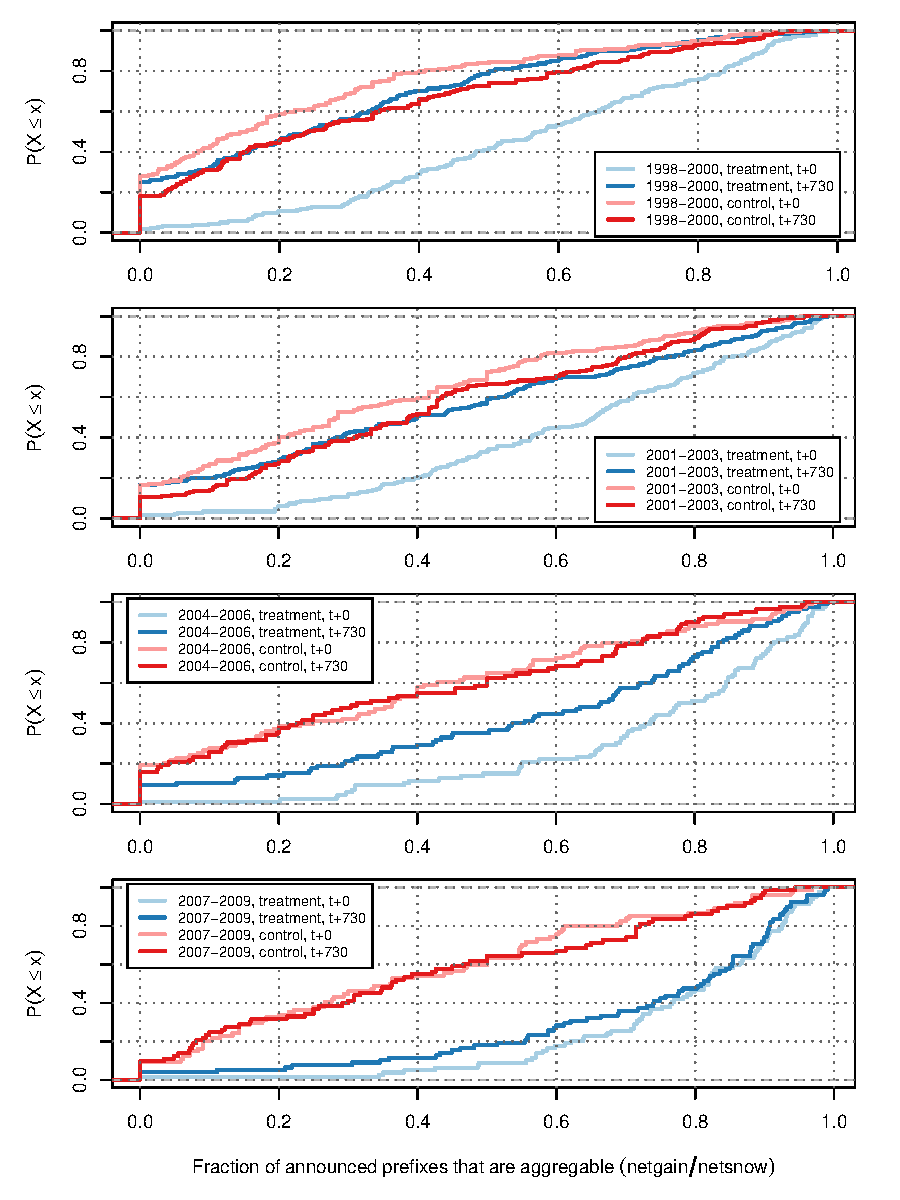
\includegraphics[width=6in]
        {figures/behavior-frac_deagg-vseries-special_tc.pdf}
    \vspace{-2em}\\
    \caption{}
\end{singlespace}
\end{centering}
\end{figure}





\begin{figure}[H]
\begin{centering}
\begin{singlespace}
    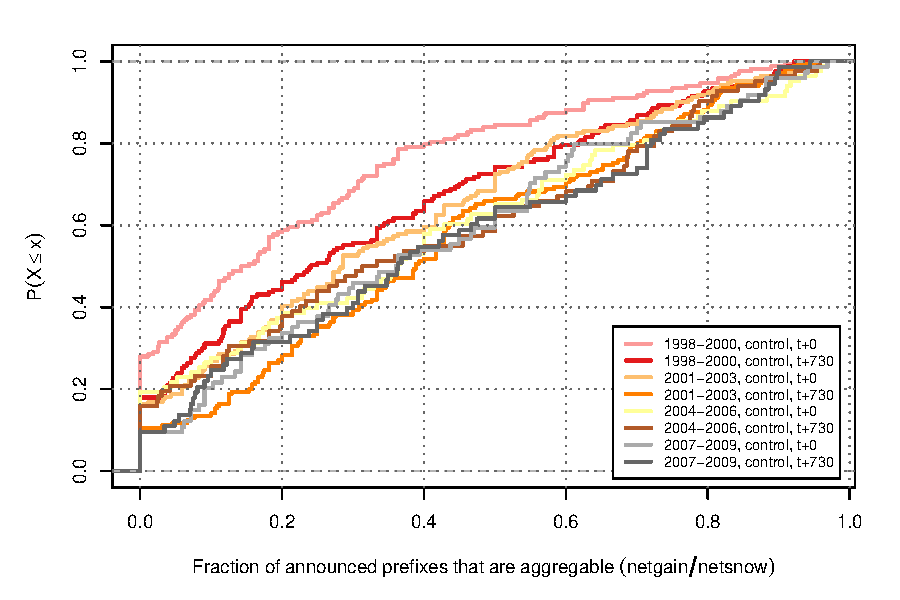
\includegraphics[width=6in]{figures/behavior-frac_deagg-all-special_c.pdf}
    \vspace{-2em}\\
    \caption{}
\end{singlespace}
\end{centering}
\end{figure}

\begin{figure}[H]
\begin{centering}
\begin{singlespace}
    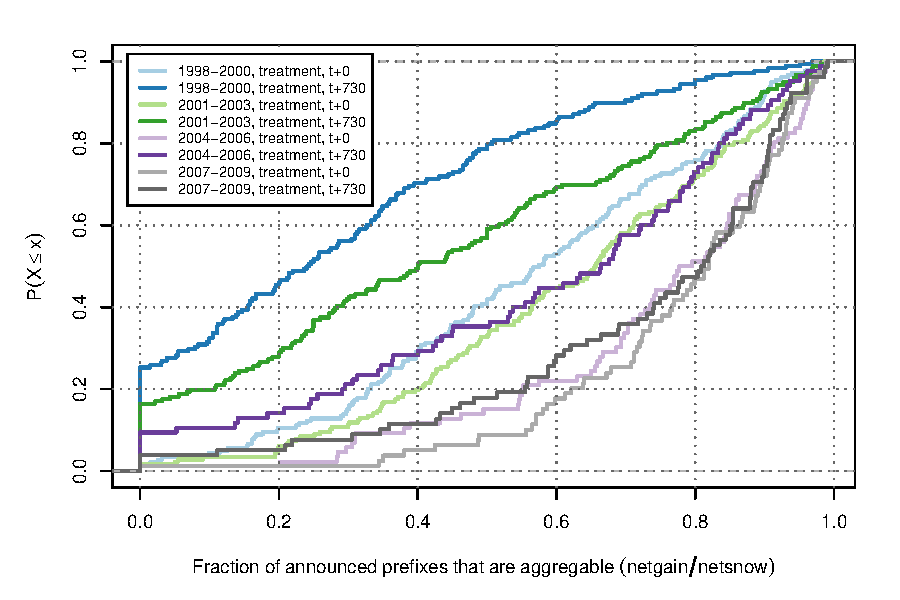
\includegraphics[width=6in]{figures/behavior-frac_deagg-all-special_t.pdf}
    \vspace{-2em}\\
    \caption{}
\end{singlespace}
\end{centering}
\end{figure}


\subsection{\fbox{TODO: Notes on validity}}
It is still difficult to tell whether the CIDR Report is having an effect -- how
do we know we are not measuring something else coincident with the CIDR Report?
This is difficult to address... Look at large-netsnow with low-netgain
population??? Future work.

It was an oversight that I did not measure behavior of ASes before their
appearance on the CIDR Report. However, because appearance is determined based
on netgain behavior means this is likely as not as huge a challenge to validity
as I expected. I still need to be concerned that appearance did not occur
because someone else got less bad, but in such a case ones aggregation
fraction would be at best flat, not decreasing to start (or they should have
appeared earlier).

% valdiity notes
% - look at CDF of population elligible to be control
% CIDR Report overall behavior notes
% -> SELECT * FROM get_cumulative_ecr_asns();
% -> SELECT * FROM cumulative_gcr_as_counts;

%%%%%%%%%%%%%%%%%%%%%%%%%%%%%%%%%%%%%%%%%%%%%%%%%%%%%%%%%%%%%%%%%%%%%%%%%%%%%%%%

%ANALYSIS
%
%- Available data/data overview
%	- plot 'h' plots of available data
%
%- Accuracy/error of my implementation of the CIDR Report
%
%- Visualization of aggregate behavior and general characteristics (in particular stratification at the top of the CIDR Report)
%    - Definition of metrics used in the analysis
%        - rank on CIDR Report (order by netgain)
%        - absolute/delta netgain
%        - relative/delta netgain (relative to netsnow)
%    - CDFs by AS appearnace
%    - CDFs by rank
%
%    - Summary/general statistics and characteristics of behavior over time (time series?), across and within groups, etc. (p62)
%
%- AS Behavior after appearing on the CIDR Report
%	- Distribution of AS behaviors from T=0, T=+1 month, 3 m, 6m, 1y, 2y, etc.
%		- all appearances on the CIDR Report
%		- no appearance/randomly selected control
%		- appearances that actually had behavior changes observed
%	- slice by date (NOT by rank on CIDR Report), and by netsnow
%
%- Variance in views of data from different peers
%- for different origin ASes that appear on the CIDR Report
%- across the entire routing table
%
%////////////////////////////////////////////////////////////////////////////////
%////////////////////////////////////////////////////////////////////////////////
%////////////////////////////////////////////////////////////////////////////////
%
%DISCUSSION
%
%Discussion of the design assumptions, and the sensitivity of the CIDR Report to those assumptions

\chapter{The CIDR Report as a mechanism for inducing collective action}
\label{chap:discussion}

% THE ENTIRE AND SOLE POINT OF THE DISCUSSION SECTION SHOULD BE TO INTERPRET
% THE RESULTS AS TO WHETHER THE CIDR REPORT EVER WAS EFFECTIVE AND THEN, BASED
% ON THE OBSERVED CHANGES, WHETHER IT BECAME LESS EFFECTIVE OR WHETHER
% SOMETHING ELSE CAUSED THE OBSERVED BEHAVIORAL CHANGE
%
% \fbox{Look at Tony Li's interview again}

The figures and analysis presented thus far have provided some insight about
the behavior of ASes appearing on the CIDR Report and general characteristics
about the CIDR Report itself. However, the process of re-implementing the
aggregation report and analyzing and observing AS behavior changes has also
raised a number of broader and more qualitative questions about the report
that we address in this chapter. We first discuss whether the CIDR Report was
accurate and whether it was effective using broader definitions of these terms
than were used in the analysis proper, and then discuss potential hypotheses
for why the response to appearing on the CIDR Report changed over time, both as
observed during the analysis and as claimed qualitatively by network operators.
Finally, we consider the CIDR Report and Internet routing table CPR in the
context of Ostrom's design principles for CPR governance institutions.

\section{Is the CIDR Report accurate?}
While part of the first section of the previous chapter was dedicated to the
question of whether our implementation of the aggregation report produced
similar output to that of the authoritative CIDR Report, we did not address the
larger questions of whether the CIDR Report is representative of the problems
observed by operators regarding deaggregation and routing table growth. These
issues are important to the CIDR Report's efficacy and trustworthiness as a
monitoring tool in support of the social forces influencing Internet routing
and aggregation, and yet are not definitively addressed; there is simply a lack
of obvious complaints or criticisms from network operators in public channels.

\paragraph{Is the CIDR Report's vantage point representative?}
The first observation we make is with regard to representativeness of the
routing table and aggregation potential observed and presented on the CIDR
Report as compared to what other network operators observe in their own routing
tables. The nature of BGP and policy-controlled route selection and propagation
make it possible for two networks to have different views and different numbers
of prefixes in their ``full'' routing table, due to the routing policies of the
networks they interconnect with. Ostensibly if the CIDR Report reports behavior
that does not represent what most other networks observe, the CIDR Report will
be less credible and more likely to be disregarded by network operators.
Unfortunately it is difficult to characterize what a representative routing
table might contain precisely because of this nature of BGP.

It would seem that the default-free zone (DFZ), the routing table maintained by
the major default-free providers that form the root of our roughly-hierarchical
Internet, is a reasonable place to take this measurement from. DFZ network
operators must theoretically maintain the fullest routing tables in order to
achieve full Internet reachability, and versions of these routing tables are
shared with DFZ customers. In cases of interactions between large
non-DFZ networks, such as major content provider or ``eyeball'' networks,
routes may be observed that are not globally visible, but it is reasonable to
expect problems related to excessive routes advertised between peers to be
resolved via normal peering dispute resolution approaches.

Reasonable proxies for the DFZ have been used as vantage points for the
authoritative CIDR Report since its inception, as identified in
Table \ref{table:cr_vantage_points}, as well as the analysis in this thesis.
However, the DFZ routing table may still not be completely representative.
Large providers receive routes from many peers and other providers, and so must
maintain a RIB that is several multiples larger than the DFZ operational
routing table or FIB, which is composed of only the best routes from the RIB.
Further, the route export policies of ISPs adjacent to the vantage point for
the CIDR Report may also affect the degree to which the CIDR Report represents
most providers routing tables. For example, in our analysis using Route Views
as a vantage point, there were cases where the DFZ and other large providers
all reported similar numbers of prefixes, while a smaller Route Views peer
reported an order of magnitude more. These additional prefixes appeared to be
in support of traffic engineering, and the AS that was ``leaking'' these
prefixes into Route Views was likely not respecting a NO-EXPORT policy that had
been applied to these routes from their origin AS\footnote{This problem was
confirmed to affect the authoritative CIDR Report as well, through indirect
correspondence with Patrick Gilmore.}. Thus, without knowing the configuration
of the export policy of peers and other providers that contribute a large
fraction of the routes to the BGP view of the vantage point, it is possible
that a non-representative view of the routing table may be generated, leading
to a non-representative CIDR Report.

% -best path only -- potentially blocks aggregation
% -filtering vs. everything for an anlytics perspective
%      Route export policy for customers vs. for CIDR Report -- i.e. routeviews
%     - no-export and other communities
%     -consensus vs. a single source vs. something in between
%
% \begin{quote}
% P.S. The list is not 100\% correct.  For instance, tw telecom has
% no-export set on their de-agg prefixes.  This means those de-aggs don't hit the
% global table, just their transit provider.  But if Geoff peers with the transit
% provider directly, he may see them (even though he should not).  I have spoken
% to tw telecom about this face-to-face.  (Part of that "shaming" thing.)
% \end{quote}

\paragraph{Is all deaggregation equally problematic?}
All route announcements that consume slots in the routing table incur the same
cost in that they consume a fraction of the router's resources that cannot be
utilized by another route. However, as the Internet has changed in purpose and
structure over time, the need to perform certain tasks (multihoming, TE) in BGP
that result in route deaggregation and increased numbers of prefixes in the
routing table have been motivated by network management and engineering. The
norms of the Internet operations community appear to have recalibrated
accordingly, seemingly assigning different value to the benefit and
justifiability of different deaggregation-inducing behavior.

While there are different views on the subject \cite{Li:2011vn}, most seem to
conclude that route announcements due to multihoming and prefix hijacking
prevention are unavoidable and justifiable, while traffic engineering is less
so, especially in the case of fine-grained TE by large residential access ISPs
\cite{Steenbergen:2010nx}. Worst of all is the failure to aggregate or
announcement of ``class C'' blocks in the era of CIDR. Such behavior indicates
a lack of ``clue'' and provides no benefit to anyone, and so is universally
deplored.

Distinguishing between these behaviors is often difficult, as the information
required to discern the intent of deaggregation is not always available from
the vantage point routing tables accessible for measurements. \cite{Bu:2004fk}
present a definition for measuring multihoming and \cite{Cittadini:2010pi}
present some measurement techniques for observing traffic engineering. However,
other forms of traffic engineering between large ASes may not be visible
because it is based on routing parameters such as NEXT\_HOP that are not
visible from adjacent ASes \cite{Steenbergen:2010nx}.

Regardless of the measurability of these various phenomena, the CIDR Report
does not attempt to measure or distinguish between any of the causes or
underlying intentions of deaggregation, instead simply reporting the number of
prefixes announced by each AS that appear aggregable from the CIDR Report's
vantage point. While this is a true representation of each AS' contributions to
the routing table, it does not accurately reflect the relative values
attributed to aggregation by network operators. Thus, some operators may
conclude that the report is not as useful because it does not distinguish
between these behaviors. Further, because some of these
purposefully-deaggregated routes are difficult to withdraw, they may lead to
some ASes appearing in unmoving positions on the CIDR Report, as hypothesized
in \cite{Steenbergen:2010nx}.

\section{Is the CIDR Report effective?}
While the section of the previous chapter analyzing the post-treatment behavior
of ASes appearing on the CIDR Report addressed the question of whether the CIDR
Report appeared to correlate with AS behavior change, it did not address the
more general question of the CIDR Report's purpose and use by operators:
initially to encourage aggregation following the adoption of CIDR and BGP-4,
and then later and more generally to encourage efficient route announcements by
providing monitoring information about the greatest deviation from community
norms.

While the validity concerns identified previously limit our ability to draw
strong, causal conclusions, it does appear that the CIDR report had some effect
on the aggregation behavior of individual ASes, especially early on in the
study period. Further, in the very early days of CIDR, there is evidence of the
total number of prefixes in the routing table actually decreasing over time as
aggregation occurred. However, during the period studied in this thesis, the
routing table generally grows continuously over time, as was shown in Figure
\ref{fig:huston_table_plot}.

\paragraph{Considering the counterfactual (no CIDR Report) world}
The ideal measure of general CIDR Report efficacy would be to observe route
announcement and aggregation behavior in the counterfactual world where the
CIDR Report does not exist. While we cannot actually observe this, we can
construct an estimate of the counterfactual routing table under the assumption
that without a CIDR Report, networks might not withdraw announcements, instead
leaving them in the routing table. By observing the cumulative number of
prefixes advertised for at least some period of time, we could construct an
upper bound of the counterfactual routing table size. A plot of these
counterfactual routing table sizes is shown in Figure \ref{fig:counterfactual}.

\begin{figure}[h]
\begin{center}
    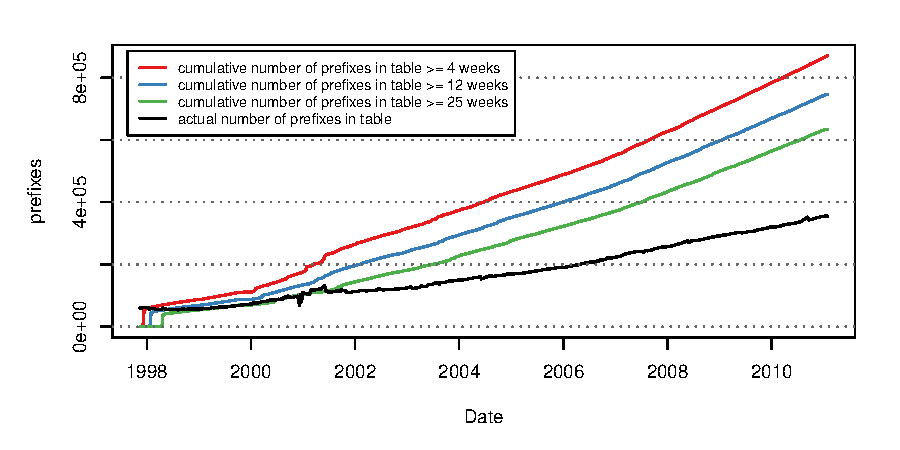
\includegraphics[width=6in]{figures/counterfactual.pdf}
    \vspace{-2em}\\
    \caption{Counterfactual routing table prefix counts over time.}
    \label{fig:counterfactual}
\end{center}
\end{figure}

As illustrated in this figure, the number of prefixes in the counterfactual
table size grows faster and eventually larger than the actual routing table
size, even for conservative estimates of how many weeks a prefix must be in the
routing table for it to constitute a ``permanent'' prefix. While the
construction of this counterfactual is far from methodologically perfect, it
provides further evidence that the CIDR Report or some other aspect of the
network operations community had some effect on route aggregation behavior. The
deviation between this counterfactual plot and the actual size of the routing
table could alternately be interpreted as evidence that there is a tendency
for aggregation or route withdrawal to occur naturally without appearing (or
fear of appearing) by the CIDR Report, though this is disputed by the behavior
of the control group in the previous chapter.

% In spite of seeing aggregation behavior relative to the control, the total
% number of routes in the routing table does not drop over time, suggesting that
% old people are replaced by new ``bad guys'' or new entrants. Cittadini's study
% suggests that the proportion of ``bad guys'' remains the same over time (the
% people that would show up on the CIDR Report), suggesting the rolling-over bad
% guy theory.
%
% OR. The table just grew less quickly than it otherwise could have, but we can't
% examine the counterfactual world...?
%
% Rolling-over bad guy theory would be supported by the rate of growth of new
% ASes on teh CIDR Report?
%
% Arthur suggests looking at the fraction (\# of /24s / \# of prefixes in the
% routing table) per AS or for the entire routing table, over time
%
% What do Cittadini's observations mean for my analysis of the later repport
% where people are far more deaggregated

\paragraph{How quickly should the CIDR Report take effect?}

This is a minor observation, but there is a question that arises from observing
the metrics selected for measurement in the previous chapter over time, such as
in Figure \ref{fig:delta_rel_netgain_cdf}. From this and other figures
presented over the various measurement periods from 30-730 days after the
initial appearance on the CIDR Report, we can see that some improvement (and
more generally change) occurs after 30 days, and often continues up to 730 days
after, though most of the observed change appears to occur between 30 and 365
days rather than than 365 and 730 days (one and two years). It seems reasonable
to assume that because most of the net change was observed to take place in the
first year after the initial CIDR Report appearance, it was likely related to
appearing on the CIDR Report and not some other phenomenon such as regression
to the mean. However, this argument is somewhat speculative in that we do not
understand the underlying mechanisms that cause the behavior changes observed.

% As those that have been treated by the CIDR Report have become more outliers
% over time, it's possible that those below the outliers may have been more
% susceptible to treatmetn. Or, they may have moved on tehir own -- it would be
% interesting to sample those with netgain comparable to 1998 CIDR report from
% 2011 and see if the behavior is more similar to 1998 or 2011.

\section{What caused the decrease in treatment effect over time?}
If we agree that there was a behavior change by ASes in response to appearing
on the report, then as we see the diminishing difference in behavior change
over time in the previous chapter, we conclude that the governance system
influenced by the CIDR Report became less effective over time. This agrees with
operator observations about the decline of the CIDR Report. However, these
observations do not offer any insight about what may have occurred within the
interdomain routing system and the Internet operations community surrounding it
to cause these changes.

Ostrom's model of rational appropriators, introduced in Chapter
\ref{chap:intro}, sets out four factors that influence the behaviors and
decision-making of appropriators. These are:
\begin{itemize}
    \item{internal discount rate: the relative perceived value of future
    benefits versus present benefits}
    \item{internal norms: internal values that influence the selection and
    relative valuation of strategies (which may in part be the result of
    externalizing internal norms)}
    \item{external costs: costs incurred from a particular strategy}
    \item{external benefits: benefits gained from a particular strategy}
\end{itemize}
By considering external changes and events over the course of the study period
that may have influenced these factors, we may be able to develop hypotheses
for the observed behavior change. While we cannot conclusively attribute the
observed behavior change to any or all of these hypotheses, they are certainly
potential causes that could be investigated further in future.

In Ostrom's work, the discount rate is typically used to describe the ease by
which an appropriator may make their livelihood from another resource system,
thus freeing them from considering the future consequences of opportunistic
behavior in the current resource system.  In the case of the routing table and
the Internet more generally, there is only one, and so we will not consider the
internal discount rate, instead focusing on the other three factors in turn
below.

\paragraph{Changing community norms and responses}
While the criterion that Ostrom identifies here is internal norms, it could be
argued that most of the internal norms of participants in the Internet
community are motivated by the collective norms of the community. We thus focus
on these specifically.

In its very early days, the Internet operations and engineering community was
relatively small and homogeneous. Consisting of groups such as the IETF or the
NSFNET Regional Techs group (the forerunner of NANOG), these groups were
relatively small, met in-person frequently, and otherwise kept in close contact
via email mailing lists. These groups were composed of relatively consistent
participants that were mostly American and affiliated with equipment vendors,
service providers, contractors, and organizations that operated
Internet-connected networks---academic and educational institutions.
Individuals and their organizations had reputations to maintain in the Internet
meritocracy, and without motivation by commercial and competitive forces, this
community was more focused on collective welfare than on individual benefit
\cite{Li:2011vn}.

As the Internet has grown over time, the operations and engineering community
surrounding and supporting it has also grown and changed. First, as the
Internet has grown in importance and deployment outside of the United States,
the community of operators that participate in BGP operations has grown to
include a much more diverse group of people that no longer meet together or
participate on the same mailing lists, or who even speak the same language or
hold the same cultural norms and values. While there are still strong and
vibrant operator communities such as NANOG, RIPE, etc. these are all generally
regional rather than global. Further, and perhaps more important is that with
the transition of Internet service provision to a highly competitive commercial
activity, considerations of the benefit or cost of a particular activity to the
community are no longer considered, or at best considered after
profit-maximizing activities \cite{Li:2011vn}. Under such a mindset, reducing
ones impact on the routing table would at best be not in support of an ISP's
core business and at worst could be viewed to harm their Internet operations,
and so aggregation has become less of a concern to large, modern ISPs.

% - community has grown and become less homogeneous
%     - originally IETF + Regional-Tech, etc. with a common ethos, frequent
%       meetings (Tony Li)
%     - now all over the world (harder to communicate), commmerically motivated
%         - still pockets of this -- NANOG, etc.
%         - the inner circle of operators is still probably strong and pwerful
%     - clue doesn't matter anymore -- no longer a pride issue.

Finally, the attitude that the CIDR Report had become ineffective, espoused by
many of the operators that we spoke with, may have also played a role in the
change in effectiveness of the CIDR Report. Given that it only provides
information, the CIDR Report may only help improve aggregation of the routing
table through social action in the Internet operations community. If leading
operators deemed the report to have become ineffective, then there would be
little reason for them to continue to apply pressure via social forces, as it
would be a waste of time, or others would free-ride off of their efforts. Thus,
if this attitude was pervasive, it may have been a self-fulfilling prophecy
that changed attitudes and responses to the CIDR Report.

% source of ossification?

\paragraph{Changing benefits of routing deaggregation}
As discussed earlier, there are now greater engineering motivations to utilize
deaggregation to achieve reliability or performance goals via multihoming,
traffic engineering, and separate announcement of critical infrastructure
addresses to avoid route hijacking. While there are questions about the degree
to which this behavior has changed over time \cite{Cittadini:2010pi}, these
behaviors are certainly considered a normal part of BGP network operation now
whereas there were arguably less critical and more unusual in the era of a more
hierarchical Internet \cite{Labovitz:2010zr}.

Perversely, it has also been claimed (but not substantiated) that appearing on
the CIDR Report has been viewed by some as a positive indication for marketing
purposes \cite{Smith:2006vn}, presumably because it suggested that one operated
a large network like others appearing on the CIDR Report.

\paragraph{Changing costs of routing deaggregation}
The costs of routing deaggregation also appear to have changed over time, both
in terms of the marginal cost of a slot in a modern router and in terms of the
community response to operating a highly deaggregated network. First, in terms
of the marginal cost of a route, typical modern routers now have capacity for
several million routing table entries. This demand for routing table slots has
apparently been driven by the popularity of BGP/MPLS VPNs \cite{rfc2547} and the
business models they enable for ISPs, leading to the present where major
customers of a prolific router vendor do not seem to express concerns about the
Internet routing table's contributions to the total demand for routing table
slots \cite{Davie:2011uq}. This has made each routing table slot less valuable
over time. While aggregable prefixes still consume a significant fraction
of the total prefixes in the Internet routing table, the benefit of taking
action to encourage others to aggregate their routes has likely decreased over
time as slots have become less scarce.

In addition to the decreased cost of routing table slots, it appears that the
community response to announcing aggregable routes has decreased over time,
making it less costly in terms of reputation and criticism to announce
deaggregated prefixes. It is not possible to observe a measure of all
criticism in response to the CIDR Report, but we can consider a reasonable
proxy---the public discussion of the CIDR Report on the NANOG mailing list. A
figure of the frequency of mail messages containing ``CIDR R'' in the subject
line over the study period is shown below in Figure \ref{fig:mail-freq}.

\begin{figure}[h]
\begin{center}
    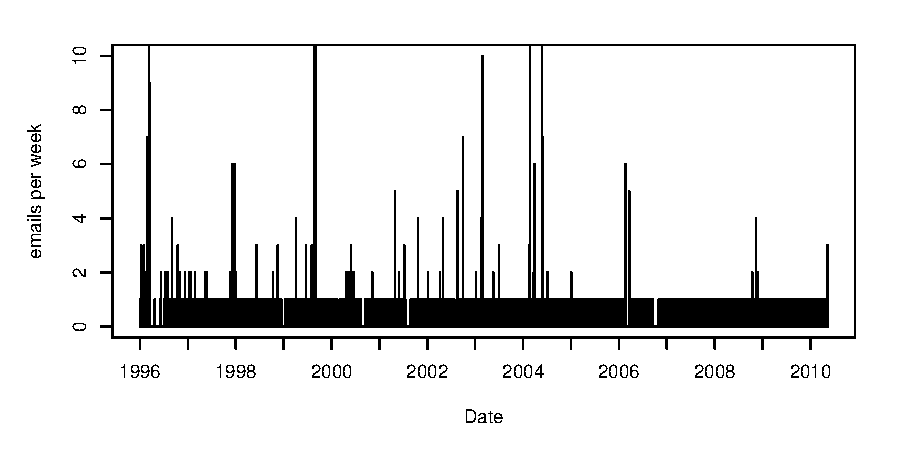
\includegraphics[width=6in]{figures/cr_email_freq.pdf}
    \vspace{-2em}\\
    \caption{Incidence of email messages containing ``CIDR R'' in the subject
    line, transmitted to the NANOG mailing list over 1996-2011.}
    \label{fig:mail-freq}
\end{center}
\end{figure}

This figure illustrates that while email discussion of the weekly CIDR Report
was fairly vigorous (including both commendations for improvement and criticism
for getting worse), these comments and conversations have essentially stopped
completely as of late. While this is probably coupled to the changes in
community norms discussed above, it also suggests that the criticism and thus
reputational ``cost'' of appearing on the CIDR Report has decreased over time.

\section{Learning from the CIDR Report and the routing table CPR system}

In spite of our discussion of governance institutions and Ostrom's CPR
framework at a number of points throughout this thesis, it is important to note
that the CIDR Report itself is not a CPR governance institution as Ostrom's
framework defines them. As noted in the introduction, such institutions require
participants to agree to make commitments to certain behavior, and typically
offer graduated sanctions to prevent opportunism in the event that monitoring
activities show deviation from commitment. In this context, the CIDR Report
fills a monitoring role that feeds into the loosely defined governance
customs that have been developed by network operators participating in the
Internet.

Ostrom \cite{Ostrom:1990fv} identifies five design principles\footnote{
The five identified for credible commitment are: clearly defined boundaries,
congruence between CPR rules and conditions, collective choice arrangements,
monitoring, and graduated sanctions. Ostrom also identifies three other
principles that, when absent, have caused failures in other CPR governance
institutions: dispute resolution mechanisms, recognition and non-interference of
the right to organize, and the use of nested enterprises in large-scale
systems}
necessary for participants in a CPR to make credible commitments to
follow agreed-upon rules. We discuss principles particularly relevant to the
CIDR Report and routing table governance institution below, while only touching
on principles that are less relevant or already satisfied.

% learning from the CIDR Report
% - not actually a governance institution -- just something some people created
%       -- maybe part of one, but AFAWK, it is completely norm-based -- there was
%       no collective action to supply an institution in the first place

\paragraph{Collective choice}
Perhaps the biggest challenge facing both the CIDR Report and the community
norm-based approach as a method of managing routing table growth is that none
of these mechanisms or the rules or principles that underlie them were ever
explicitly agreed upon or developed through a process by participants in the
interdomain routing system. Thus, when the community shared a collective set
of norms and principles regarding maintaining reputation, minimizing
deaggregation, etc., the CIDR Report provided a monitoring service according to
these norms and identified ASes that deviated from them most significantly.
With this information, community members who shared these norms could then
apply social pressure or assist the deviating ASes in improving their
aggregation behavior.

However, as these norms changed and the community also changed, there was no
precedent or process by which to achieve collective action to adjust the rules
to meet these changes and the interests of network operators accordingly. Thus,
the CIDR Report could not necessarily evolve to meet the interests of all, and
there was no obvious venue for network operators to participate in order to
change the CIDR Report or the rules and expectations of the community. Ostrom
would suggest that these reasons lessen the incentive for individuals to commit
to the rules of the routing table CPR, and ostensibly also played a role in the
apparent reduced efficacy and relevance of the report over time.

\paragraph{Monitoring}
The design principle most relevant to the CIDR Report is that of monitoring, as
it is the primary role of the CIDR Report. Monitoring, along with sanctions,
are essential to maintaining cooperation and limiting opportunistic behavior in
the long-running CPR institutions that Ostrom observes opportunistic behavior,
even in communities with shared norms and interest in reputation maintenance.
Internal monitoring and sanctioning provide assurances to participants making
commitments to abide by the rules that their trust will not be taken advantage
of---that opportunists will be detected and punished.

In consideration of Ostrom's principles, the CIDR Report is a reasonable
monitoring mechanism: it is provided by and can be verified by participants,
and is of low cost relative to sanction mechanisms. However, it is not ideal,
especially as it has remained static while the Internet has evolved.  In
addition to the specific issues of vantage points, accuracy, and interpretation
mentioned earlier, the CIDR Report only identifies the thirty most extreme
deaggregators in the network each week. While a limit on the number of networks
identified each week is arguably necessary because the social response to the
CIDR Report is a necessarily a human process that can only cope with a limited
amount of information, it has not scaled as the Internet has grown. Instead, as
illustrated in Figures \ref{fig:netcompare} and \ref{fig:netgain_cdf}, it now
focuses on significantly deaggregated outliers---0.1\% of the routing system
participants with 20\% of the prefixes.

This group of outliers may indeed be deserving of community attention, but the
limit of 30 ASes also ignores the next 20\% of the population that is
collectively responsible for the remaining 80\% of the aggregable prefixes.
These participants may be significantly deaggregated in relative terms and may
be in positions to easily improve their aggregation behavior but, because of
their relative size, never appear above the threshold of thirty. With the
current and historic trend of a constantly increasing minimum threshold to
appear on the CIDR Report, an AS just below this threshold could easily avoid
social pressure and criticism while not committing to the broader norms that
the CIDR Report embodies.

\paragraph{Graduated sanctions}
Given that the CPR governance institutions observed by Ostrom typically
involved communities with frequent and repeated interaction, her studies found
that graduated sanctions---small sanctions for first or infrequent offences and
larger sanctions for later or more frequent deviations---were important for
achieving a stable, cooperative appropriation institution. Sanctions, while
more expensive than norms in establishing order, help to ``backstop'' norms in
cases where the benefits of opportunism exceed the costs of contravening norms.
The CIDR Report and routing table CPR system has two significant shortcomings
with regard to sanctions.

First, there are no strong, guaranteed sanctions in response to appearing on the
CIDR Report. Beyond the shame or fear of reputation loss motivated by internal
norms in response to appearing on the report, there is only the explicit
criticism of others to motivate changes in aggregation behavior in order to
reduce ones ranking on the report. This is not coordinated in any way, and
instead relies on other participants to respond to the CIDR Report mail message
by apply pressure or criticism via public email response, private
communication, or in-person discussion at the next operator meeting (i.e.
NANOG). It is possible that operators could use existing business relationships
and contracts to apply leverage to other networks to improve their aggregation
behavior in a way that is private, but this was not encountered in our study of
mailing list archives or discussion with operators.

In addition, these social sanctions are not particularly graduated. They are
not applied consistently across all ASes, nor are they applied in an organized
fashion, but again rely on other operators to apply pressure as they choose to
or are able. Further, while it is doubtful that an AS ranked in the 30th
position on the CIDR Report receives the same attention as the first-ranked AS,
their identification is at least publicized, compared to the AS ranked 31st who
may have very similar behavior but not appear at all on the report.

% This suggests that automated sanctions or pricing might be more effective.
%
% The challenge of agreeing to supply an institution that does anything more
% than provide information (i.e. sanctions) multilaterally is potentially
% problematic in looking beyond the CIDR Report.
%
% Interconnection is voluntary -- libertarian vs. collectivist thought

\paragraph{Other design principles}
The CIDR Report and associated norms of the Internet routing table also do not
incorporate a number of Ostrom's other design principles:

\begin{itemize}
\item{Clear boundaries: while the interdomain routing system is limited to BGP
speakers, there is no boundary that limits routing slot appropriation to those
that adhere to the community norms only.}
\item{Rules suited to actual conditions: as alluded to earlier with regard to
collective choice, the norms embodied in the CIDR Report have not evolved as
routing table slots have become less scarce and deaggregation-causing
activities are common BGP operations, and so probably no longer represent the
norms and concerns of the community.}
\item{Nested enterprises: this technique is used to achieve scalability in CPR
governance institutions by organizing local institutions that then participate
in a larger regional/etc. institutions. Such nesting may occur informally via
regional operator groups and RIRs, but the CIDR Report is a global activity.}
\end{itemize}

\paragraph{Conclusion}
Given these observations that the CIDR Report and the loose, norms-based
governance approach used by participants in the interdomain routing system do
not realize most of Ostrom's empirically-derived design principles for
long-standing CPR governance institutions, it should probably not be a surprise
that the report has become less effective over time. It is difficult to compare
the CIDR Report to other CPR situations, but perhaps it should even be
considered remarkable that it was effective for as long as it was without a
solid foundation as Ostrom would have prescribed. Regardless, it seems apparent
that the lack of some of these principles, such as collective choice and
sanction mechanisms, would have been important in allowing the CIDR Report to
remain effective.

% \paragraph{Other design principles}
%
% followed principles, in addition to monitoring
% - right to organize (i guess so -- no antitrust/etc issues it seems)
%
% missing principles, in addition to sanctions
% - clear boundaries -- while it takes a modicum of clue to particiapte in
%   interdomain routing, participating requries no agreement to norms to
%   participate
% - well-tailored rules; no -- essentially no shame if you're below the CR
%   threshold
% - conflict resolution? never really an issue yet -- probably more essential if
%   sanctions were serious or otherwise there was concern over interpretation or
%   behavior
% - nested enterprise -- no, currently this is global, even though there are
%   regional network operator conferences
%     -- shared values and different problems for different
%       appropriators
%
% - regional rescaling to achieve nested enterprises -- bringing people who can
%     easily communicate and affect eachother and be aware of local conditions
%     together. how does this scale to the internet? sort of would work with
%     regional operator communities, but what about the organizations that
%     transcend regions -- do they have an obligation to attend all of these
%     things?
%
% - related to the above -- shared values/norms
%     erosion of traditional ones -- ostrom sez this is important
%         While the norms and values embedded in the Internet community may have
%         been helpful in past, it's not clear that these are or will continue to
%         hold (cite Tussle in Cyberspace) and so we probably shouldn't expect
%         the CIDR report to work in the same way, especially with expansion into
%         other regions where the culture/Internet ethos isn't the same, or where
%         people aren't aware of the history, or loosely/not-at-all connected to
%         the community that does still exist.



\chapter{Related Work}
\label{chap:relwork}

The important central role played by interdomain routing in the Internet, along with the problems that many have seen emerge in this space over time, has caused this topic to be a focus of much work on the part of academic researchers, network equipment vendors, and network operators. This work can be classified as that which is specifically focused on the problem of growth of the routing table due to network operations, as well as work more broadly focused on the problems of our current interdomain routing architecture. Both of these topics are discussed in more detail in following sections. A section on the limited literature and other information about the Internet operations community and its norms, ethos, and characteristics is also included because of the importance of this community in producing the social forces that could make the CIDR Report effective.

Note that sources from the Internet operations community, while perhaps less academically credible because they are typically not published in traditional peer-reviewed forums, are included here and elsewhere in this thesis because they are extremely valuable for gaining a more thorough and comprehensive understanding of this topic.

% major hole -- methodological literature

\section{Analyses of routing table growth \& deaggregation}

Some of the work in this space has been devoted specifically to the topic of the Internet routing table, arguably because it's both the immediate source of scaling problems and because it's something that researchers, vendors, and operators all think about. This work has generally focused on characterizing the growth of the routing table over time and attempting to understand the sources of or reasons for the growth. These works often mention the CIDR Report as a source of information but do not discuss its efficacy.

Beyond some of the ad-hoc analysis that took place during the supernetting \cite{rfc1338} and ultimately CIDR \cite{rfc1519} design and deployment, \cite{Huston:2001bs} is one of the first works analyzing the Internet routing table. In this paper, Huston analyzes the size and growth of the BGP routing table from 1988-2001 and identifies four phases of growth surrounding the deployment of CIDR. He finds that while CIDR deployment did reduce the size of the routing table and limit the exponential growth preceding its deployment to linear growth shortly after, growth did ultimately return to exponential again as the Internet grew in commercial importance starting in the late 1990s. While not specifically determining the contributions of various factors to the observed growth, he does note that traffic engineering and multihoming are increasing over time. Huston concludes by casting the problem as a ``tragedy of the commons'', lamenting that the usual solution of a central regulator is not obviously available to a globally distributed system like the Internet. Interestingly, or perhaps tellingly, Huston does not acknowledge the CIDR Report as a regulatory mechanism for this role.

Bu et al. \cite{Bu:2004fk} go on to analyze the routing table with a focus on determining the contributions that a number of operational behaviors have on routing table growth: load balancing (traffic engineering), multi-homing, RIR address fragmentation, and failure to aggregate. Like this thesis, they also use Route Views as their data source, verifying that it provides a sufficiently comprehensive view of the Internet routing table. They perform an analysis of aggregation potential similar to both the CIDR Report and the analysis of this thesis, though they perform aggregation solely based on routing policy, rather than prefix hierarchy as well. The authors of this paper conclude that address fragmentation caused by RIR allocation policy was the greatest source of prefixes in the routing table as of 2002, with multi-homing, traffic engineering and failure to aggregate contributing 30\%, 25\%, and 20\% additional prefixes respectively. They also find that traffic engineering was the fastest-growing cause of routing table growth.

A more recent study by Cittadini et al. \cite{Cittadini:2010pi} provides an update about the state of routing table deaggregation and update dynamics, and also dispels some myths about where the blame lies for deaggregation in the DFZ. This is a useful and welcome update given changes in the Internet since the previous works. In spite of the Internet's evolution, they find that neither the fraction of the routing table that is deaggregated nor the fraction of ASes performing traffic engineering has changed noticeably since 2001, but instead has remained proportional to the size of the routing table. They also go on to analyze the distribution of deaggregation in different populations (i.e. ISPs, enterprises, etc.) and find that while a disproportionately small number of ASes advertise most of the routes in the DFZ, the proportion of these ``bad guys'' has not changed over time. These conclusions are interesting and present a more reasonable perspective on the data analyzed by Bu and Huston in that they consider the results relative to the routing table. %The observation that the small proportion of ``bad guys'' has remained suggests that community forces might still possibly be valuable.

In good contrast to the more academically-oriented work in this space, \cite{Zhao:2001ly} is written by a trio of experienced network operators and describes the operational concerns regarding routing table growth, as well as the challenges in implementing any proposed solution in a production service provider environment, such as the business case for upgrades and the typical 5-7 year depreciation cycle for routers and other equipment. In \cite{Steenbergen:2010nx}, Steenbergen presents another operator's perspective, taking up a number of similar hypothesis regarding the cause of table growth as in \cite{Bu:2004fk} and \cite{Cittadini:2010pi}, illustrating how these factors are indeed present in the table, and discussing operational solutions to minimize these problems. Finally, \cite{Smith:2006vn} presents the conclusions of a more qualitative study by a European network operators group, which did mention the CIDR Report and the ``CIDR Police'' (discussed below) as mechanisms to mitigate routing table growth.

%Some other analyses of note include a a small study of deaggregation behavior in \cite{Gagliano:2009zr} where, like this thesis, the aggregation behavior is analyzed at the granularity of ASes rather than the routing table as a whole. Game theoretic modelling: \cite{Kalogiros:2009ly}

\section{Improving Interdomain Routing Scalability}

Much more of the work in this space, mainly by academics and researchers, has been focused on the broader problems with our current architecture for interdomain routing. Along with problem statements, a number of technical solutions have been proposed, both incremental and radical (involving full protocol changes or clean-slate redesigns), but most have yet to gain any traction within vendor and operator communities. A few non-technical solutions based on economic incentives or operational practices have been proposed or attempted to resolve the more specific routing table growth problem. These appear to be far less popular than technical solutions to the problem, and while these ideas are often articulated in operator forums, they also have not gained any traction.

At high level, \cite{Yannuzzi:2005hc} captures a number of challenges and proposed improvements to interdomain routing within the context of arbitrary AS topologies and a BGP-like routing algorithm. \cite{Handley:2006kx}, in the context of describing a number of broader issues facing the Internet architecture, discusses the scaling and reliability challenges of interdomain routing and the even larger challenges of deploying a replacement until the incentives are sufficient to do so. In \cite{Feamster:2004nx}, Feamster et al. discuss a number of specific problems in BGP introduced by the design goals of policy routing and scalability, with the intent to direct research towards designing more robust interdomain routing protocols. The IETF and IAB have also studied the problem of routing scalability more broadly in \cite{rfc4984}, with the understanding that some of the scaling issues may come from our current architecture and instead produced broader problem statements and criteria that proposed solutions to the routing scalability problem must meet.

A number of small proposals to incrementally alter BGP-speaking routers have emerged, such as routers that discard information and retrieve it later if necessary \cite{Karpilovsky:2006ys}, and routers that aggregate their FIB internally, similar to the aggregation performed by the CIDR Report, to conserve memory without altering routing policy \cite{Zhao:2010vn}. Operational techniques are also available to operators, including route filtering based on RIR policies to limit more specific routes used for traffic engineering, etc. \cite{Bellovin:2001qf}, although this technique is likely not to be effective any more as RIRs have continued reducing their minimum allocation size with the exhaustion of IPv4 addresses. Finally, routers can also be configured to perform virtual aggregation, such as in \cite{Ballani:2009tg}, where a routing table is effectively spread across multiple routers, thus performing full lookups in two or more hops instead of one. All of these options are attractive for individual providers as immediate benefit in terms of routing table reduction can be realized without requiring coordination with others or a protocol change, and are likely to be easily implemented with a software or configuration update. However, while all of these approaches reduce the routing table size and growth rate pragmatically, they do not alter BGP's fundamental scaling characteristics, particularly with regard to update messages.

In terms of architecture-level proposals, many solutions to the problem propose to overcome the overloaded use of IP addresses as both topological locators and endpoint identifiers. It is argued that eliminating this overload would allow traffic engineering, multi-homing, and other behaviors to still occur while reducing the size of routing table, as aggressive hierarchical aggregation would be possible \cite{Quoitin:2007uq}. There have been a number of proposals in this space, but one of the more well known efforts oriented at real deployment is the Locator/ID Separation Protocol (LISP) \cite{lisp-id}, which maintains two separate (IP) address spaces for identifiers and locators, defines mappings between them for interdomain routing (i.e. which locator is the destination for a given identifier), and encapsulates packets with this appropriate mapping for interdomain routing. A more recent alternative that appears more favorable for incremental deployment is the Identifier-Locator Network Protocol (ILNP) \cite{Atkinson:2010zr}, utilizes the current IPv6 routing architecture along with DNS to provide locator-identity separation. More radical proposals such as HLP \cite{Subramanian:2005ve} and NIRA \cite{Yang:2007cr} are not incrementally deployable but offer new architectures and models that are free from the warts of BGP and its implementation and operation. 

In contrast to CIDR and many of these other proposed schemes, including locator-identifier separation, that rely on the aggregation properties of hierarchical routing, \cite{Krioukov:2007fk} claim that we need a fundamentally different approach to routing on the Internet as any hierarchical routing algorithm will not scale well when applied to scale-free ``Internet-like'' topologies. They argue instead for \emph{compact routing} that by design scales sub-linearly in the worst case, at the cost of selecting paths longer than the shortest path between any two nodes. They make their argument from a mainly theoretical standpoint, rather than one of engineering for scaling the Internet up to the next order of magnitude or within the bounds that are likely to be provided by Moore's Law and advancing router architectures. Also, they mainly consider shortest path routing rather than policy routing, which is of less interest in the context of interdomain routing on the Internet.

\section{Non-technical solutions to routing table growth \& deaggregation}

Most efforts dedicated to the problems of routing table growth and deaggregation have focused on technical improvements to single aspects of BGP routers or full-scale, clean slate shifts to interdomain routing architectures with more favorable scaling properties. However, a few efforts have considered non-technical means to manage the growth of the routing table, including routing economies (effectively internalizing the negative externality) and encouraging more effective network operations.

In the face of routing table growth, Rekhter et al. \cite{Rekhter:1997mi} argue for charging neighbors for use of slots in the routing table by establishing bilateral contracts for carrying route advertisements. They discuss the success of what they term the ``spirit of cooperation'' in operating the Internet thus far, but claim that it will not scale as the Internet grows and becomes more commercial, and also claim that it will become more difficult to come to agreement about policy governing appropriate behavior. In place of norms, they assert that the use of financial settlement allows for flexibility in route selection and advertisement based on the value of selecting non-default routes. As discussed previously, there are varying degrees of private benefit that are derived from route deaggregation, and financial settlement creates incentives to reduce non-valuable uses and allow for valuable uses to be compensated appropriately. Rekhter's proposal is complex, requiring bilateral contracts to be negotiated and executed between each pair of ASes that exchange routes between each other. Such complexity would likely hinder adoption, and especially incremental adoption, by ISPs. However, if successful such a contracting system should indeed incentivize route aggregation and efficient route announcements. Ideally, in a competitive market, the price would begin to reflect the full cost of advertising a prefix into the global routing table.

A more recent consideration of use of economic disincentives to discourage routing table growth is found in \cite{Clayton:2010bh}. In this paper, Clayton describes the challenges in appropriately charging for routing table slots, as well as the realization that to fairly apportion his estimated marginal cost of \$77,000 per route, some kind of mechanism to appropriately share fees with all networks burdened by the route is required---something that would likely amount to Rekhter et al.'s solution. 

Others, such as Zhao et al. \cite{Zhao:2001ly}, briefly discuss potential alternative business models for ISPs where cost settlements would be paid to advertise prefixes to DFZ providers, creating an economy for routing prefixes in addition to traffic. However, this proposal is dismissed relatively quickly for reasons of complexity and political feasibility with the Internet community.

Like the CIDR Report emerged from the community to inform network operators about how to better operate their networks, other efforts have also come from the community. First, in terms of education, presentations such as \cite{Steenbergen:2010nx} are relatively common at NANOG meetings, and reiterate to the community the problems associated with routing table growth while also providing operational solutions to reduce the impact of one's network on the routing table, such as advertising traffic engineering routes with a NO\_EXPORT community attribute to keep TE routes out of the routing table.  More interestingly, a volunteer effort called the CIDR Police \cite{Nussbacher:2003ys} that emerged from the NANOG community acted both in an educational role and as a more direct or explicit sanction for operators to improve their behavior. The instigators of the project claim to have had a material impact on the growth of the routing table in the 2000-2002 period.

\section{The Internet operations community and the social forces within}

There is unfortunately a dearth of work available discussing the community of Internet creators and operators, and its norms and characteristics or the makeup of its membership, in spite of the arguable importance of this group in the realization and continued functioning of the Internet. Some insights can be gathered from a thesis \cite{Mathew:2009dz} and a follow-on paper \cite{Mathew:2010ly} that studies the social interactions between network operators in the context of BGP operations. In these works, Mathew finds that operators organize loosely based on reputation and network stature in the Internet topology, and have traditionally expected other ``clueful'' operators to operate their networks competently.

Broader discussions of the Internet ethos and the nature of the (academically-oriented) community that was involved in the founding and growth of the ARPANET and NSFNET, the networks that later became the Internet as we know it today, can be found in some of the historic and ethnographic accounts of the Internet's origins. First among the work in this area is Abbate's \emph{Inventing the Internet} \cite{Abbate:2000ve}, and Hafner's slightly less formal \emph{Where Wizards Stay up Late} \cite{Hafner:1996qf} was also helpful.

Finally, the nature of the Internet operations community can be gleaned to some extent by reading the mailing lists that the members of the community participate in, such as \cite{NANOG}.

\section{\fbox{TODO:Collective action in protocol adoption}}

\fbox{\parbox{6in}{it seems like this the discussions of incentives for incremental adoption of protocols and ``going first'', especially with security protocols, might be useful for this discussion, but I'm leaving this here for now and may not return to it...}}
\chapter{\fbox{TODO:Conclusions and Future Work}}
\label{chap:conclusion}

\section{Is routing table growth still a problem?}
blah

%Is routing table growth still a problem? If you conclude yes, then by all accounts it will be more difficult to coordinate our way out of the next routing table growth ceiling. When you compare BGP3->BGP4 (although they were somewhat compatible) to IPv4->IPv6, the progress on the former is relatively incredible. While this may be because of the relatively greater pain that was being experienced at the time (that we haven't yet seen in IPv4), it seems like a reasonable conclusion all the same.

\section{Technical solutions to routing table growth}

ILNP may have killer apps, but not for ipv6 or routing table growth

%
%We'll need to coordinate again in some way, but how do we do that?
%- switch protocols?
%- economic solutions
%- improve social/CPR governance?
%  - need to be able to answer questions about what is "fair"? ("know it when you see it?")
%  - would something like a routing table governance council actually allow continued enjoyment of the dynamic aspects of internet routing?
%  - need sanctions (see what else ostrom has to say about this)
%    - how do you actually do this? routing, but there is a problem of adoption and market power and who has influence

\section{Non-technical solutions}

Discussion of the challenges of the changing landscape of the Internet http://portal.acm.org/citation.cfm?id=1851194

Sanctions are a challenge, and while there are some opportunities available within the routing system, the economic or operational ``damage'' that can be done is proportional to the content or customers you serve. Looking at other mechanisms for unilateral or multilateral sanctions within the Internet is a major opportunity for future work.

Economic arguments and palatability in considering replacement protocols in the IETF

Could a "cartel" of DFZ/Tier-1 providers start this because they have the disciplinary ability? We can look to the minimum prefix length requirements in the IPv4 days (more research required) and in IPv6 with the /32 minimum with Verizon, and how this got washed away by an interest in serving the market -- apparently the incentive to curtail routing table growth just isn't there...?

\section{Future Work}
Measure pre-treatment behavior (behavior before appearance i.e. T-30days...) to see if behavior changed, rather than
Use stronger statistical measures

Look at aggregation behavior moving down the list to see where a break occurs
\appendix
\chapter{Software produced for this thesis}
\label{chap:opensource}

A number of software tools were built in order to conduct the analysis undertaken for this thesis. This includes an implementation of the CIDR Report's aggregation report, as well as a number of small tools for processing routing table data, as well as conducting the analysis and producing the figures that go into this thesis. All of these tools can be found in the Git repository at the following URL:\\
\indent \url{https://github.com/woodrow/cidr-report_analysis}

\vspace{1em}
\noindent The source files used to generate this thesis can be found in the Git repository at the following URL:\\
\indent \url{https://github.com/woodrow/sm-thesis}

\vspace{1em}
\noindent Both URLs were functional and publicly available as of the date of submission of the thesis.

%\clearpage
%\newpage

\chapter{Sample CIDR Reports}
\label{chap:cidr_reports}

\section{Emailed CIDR Report}
\lstset{basicstyle=\scriptsize\ttfamily\fontsize{9.5}{9.5}\selectfont}
\begin{lstlisting}[frame=trl]
This report has been generated at Fri Nov 12 21:11:47 2010 AEST.
The report analyses the BGP Routing Table of AS2.0 router
and generates a report on aggregation potential within the table.

Check http://www.cidr-report.org for a current version of this report.

Recent Table History
        Date      Prefixes    CIDR Agg
        05-11-10    337795      206264
        06-11-10    337843      206672
        07-11-10    338022      206620
        08-11-10    338060      207433
        09-11-10    339052      207760
        10-11-10    339893      207903
        11-11-10    340203      208173
        12-11-10    340330      208528


AS Summary
         35919  Number of ASes in routing system
         15316  Number of ASes announcing only one prefix
          4556  Largest number of prefixes announced by an AS
                AS4323 : TWTC - tw telecom holdings, inc.
      101649920  Largest address span announced by an AS (/32s)
                AS4134 : CHINANET-BACKBONE No.31,Jin-rong Street


Aggregation Summary
The algorithm used in this report proposes aggregation only
when there is a precise match using the AS path, so as
to preserve traffic transit policies. Aggregation is also
proposed across non-advertised address space ('holes').

 --- 12Nov10 ---
ASnum    NetsNow NetsAggr  NetGain   % Gain   Description

Table     340755   208585   132170    38.8%   All ASes

AS6389      3751      407     3344    89.1%   BELLSOUTH-NET-BLK -
                                               BellSouth.net Inc.
AS4323      4556     1679     2877    63.1%   TWTC - tw telecom holdings,
                                               inc.
AS6503      2001      433     1568    78.4%   Axtel, S.A.B. de C.V.
AS19262     1780      316     1464    82.2%   VZGNI-TRANSIT - Verizon Online
                                               LLC
AS4766      1728      575     1153    66.7%   KIXS-AS-KR Korea Telecom
AS17488     1360      272     1088    80.0%   HATHWAY-NET-AP Hathway IP Over
                                               Cable Internet
AS22773     1242      164     1078    86.8%   ASN-CXA-ALL-CCI-22773-RDC -
                                               Cox Communications Inc.
AS4755      1385      403      982    70.9%   TATACOMM-AS TATA
                                               Communications formerly VSNL
                                               is Leading ISP
AS18566     1091      158      933    85.5%   COVAD - Covad Communications
                                               Co.
AS24560     1056      201      855    81.0%   AIRTELBROADBAND-AS-AP Bharti
                                               Airtel Ltd., Telemedia
                                               Services
AS10620     1333      523      810    60.8%   Telmex Colombia S.A.
AS33363     1560      784      776    49.7%   BHN-TAMPA - BRIGHT HOUSE
                                               NETWORKS, LLC
AS18101      905      138      767    84.8%   RELIANCE-COMMUNICATIONS-IN
                                               Reliance Communications
                                               Ltd.DAKC MUMBAI
AS7545      1438      698      740    51.5%   TPG-INTERNET-AP TPG Internet
                                               Pty Ltd
AS28573     1167      514      653    56.0%   NET Servicos de Comunicao S.A.
AS8452      1073      434      639    59.6%   TE-AS TE-AS
AS4808       922      287      635    68.9%   CHINA169-BJ CNCGROUP IP
                                               network China169 Beijing
                                               Province Network
AS8151      1345      721      624    46.4%   Uninet S.A. de C.V.
AS17676      640       66      574    89.7%   GIGAINFRA Softbank BB Corp.
AS7303       826      256      570    69.0%   Telecom Argentina S.A.
AS22047      563       31      532    94.5%   VTR BANDA ANCHA S.A.
AS3356      1191      690      501    42.1%   LEVEL3 Level 3 Communications
AS7552       642      141      501    78.0%   VIETEL-AS-AP Vietel
                                               Corporation
AS9443       571       76      495    86.7%   INTERNETPRIMUS-AS-AP Primus
                                               Telecommunications
AS1785      1799     1320      479    26.6%   AS-PAETEC-NET - PaeTec
                                               Communications, Inc.
AS14420      571      100      471    82.5%   CORPORACION NACIONAL DE
                                               TELECOMUNICACIONES - CNT EP
AS4780       713      243      470    65.9%   SEEDNET Digital United Inc.
AS4804       540       76      464    85.9%   MPX-AS Microplex PTY LTD
AS36992      650      189      461    70.9%   ETISALAT-MISR
AS6478      1392      932      460    33.0%   ATT-INTERNET3 - AT&T Services,
                                               Inc.

Total      39791    12827    26964    67.8%   Top 30 total


Possible Bogus Routes
\end{lstlisting}
\begin{center}
\emph{\ldots list of bogons removed \ldots}
\end{center}
\begin{lstlisting}[frame=brl]
Please see http://www.cidr-report.org for the full report

------------------------------------
Copies of this report are mailed to:
  nanog at merit.edu
  eof-list at ripe.net
  apops at apops.net
  routing-wg at ripe.net
  afnog at afnog.org
\end{lstlisting}

\clearpage
\section{Detailed CIDR Report}
\lstset{basicstyle=\scriptsize\ttfamily\fontsize{7}{7}\selectfont}
\begin{lstlisting}[frame=trl]
Aggregation Report: Aggregation using AS prepended PATH

Report prepared at Sat, 13 Nov 2010 04:11:55 UTC+1000, using data obtained within AS0.6447

The report may include routes internal to AS0.6447, and may also include routes
that are accepted from adjacent AS's and marked "NO EXPORT". The report also
does not take into account conditions local to each origin AS in terms of policy
or traffic engineering requirements. As an aggregation guide, this report is a
very approximate guide at best.

AS list, ordered by net reduction in advertisements

AS            AS Name                                      Current  Wthdw  Aggte  Annce Redctn       %
              Routing Table                                 347822 174358  29764 203228 144594  41.57%
AS6389        BELLSOUTH-NET-BLK - BellSouth.net Inc.          3755   3526     53    282   3473  92.49%
AS4323        TWTC - tw telecom holdings, inc.                4555   3501    461   1515   3040  66.74%
AS19262       VZGNI-TRANSIT - Verizon Online LLC              1782   1643    144    283   1499  84.12%
AS4538        ERX-CERNET-BKB China Education and Research N   1670   1428     44    286   1384  82.87%
AS6503        Axtel, S.A.B. de C.V.                           2003   1534    258    727   1276  63.70%
AS4766        KIXS-AS-KR Korea Telecom                        1866   1315    122    673   1193  63.93%
AS22773       ASN-CXA-ALL-CCI-22773-RDC - Cox Communication   1243   1184     10     69   1174  94.45%
AS4755        TATACOMM-AS TATA Communications formerly VSNL   1383   1196     29    216   1167  84.38%
AS17488       HATHWAY-NET-AP Hathway IP Over Cable Internet   1360   1210    151    301   1059  77.87%
AS6478        ATT-INTERNET3 - AT&T Services, Inc.             1392   1225    174    341   1051  75.50%
AS1785        AS-PAETEC-NET - PaeTec Communications, Inc.     1799   1146    106    759   1040  57.81%
AS28573       NET Servicos de Comunicao S.A.                  1182    948    103    337    845  71.49%
AS33363       BHN-TAMPA - BRIGHT HOUSE NETWORKS, LLC          1560   1015    234    779    781  50.06%
AS20115       CHARTER-NET-HKY-NC - Charter Communications     1552    991    216    777    775  49.94%
AS24560       AIRTELBROADBAND-AS-AP Bharti Airtel Ltd., Tel   1056    860     92    288    768  72.73%
AS18101       RELIANCE-COMMUNICATIONS-IN Reliance Communica    905    813     46    138    767  84.75%
AS10620       Telmex Colombia S.A.                            1333    963    207    577    756  56.71%
AS8151        Uninet S.A. de C.V.                             1351    933    212    630    721  53.37%
AS3356        LEVEL3 Level 3 Communications                   1204    744     31    491    713  59.22%
AS7303        Telecom Argentina S.A.                           826    776     71    121    705  85.35%
AS11492       CABLEONE - CABLE ONE, INC.                      1256    778    111    589    667  53.11%
AS8452        TE-AS TE-AS                                     1073    846    184    411    662  61.70%
AS4808        CHINA169-BJ CNCGROUP IP network China169 Beij    948    720     59    287    661  69.73%
AS18566       COVAD - Covad Communications Co.                1091    651     26    466    625  57.29%
AS7545        TPG-INTERNET-AP TPG Internet Pty Ltd            1436    823    221    834    602  41.92%
AS855         CANET-ASN-4 - Bell Aliant Regional Communicat    628    586     11     53    575  91.56%
AS17676       GIGAINFRA Softbank BB Corp.                      640    576      3     67    573  89.53%
AS4780        SEEDNET Digital United Inc.                      718    574     32    176    542  75.49%
AS7552        VIETEL-AS-AP Vietel Corporation                  642    583     44    103    539  83.96%
\end{lstlisting}
\begin{center}
\emph{\ldots middle of list (35743 lines) omitted \ldots}
\end{center}
\begin{lstlisting}[frame=brl]
AS3.644       COLOBRIDGE-AS Colobridge gmbh                      1      0      0      1      0   0.00%
AS3.641       TASJIL-PRODUCTION-AS tasjil art production an      1      0      0      1      0   0.00%
AS3.643       TEREWENKO-AS FOP TERESHCHENKO OLEKSANDR TROHU      1      0      0      1      0   0.00%
AS3.647       VSESVIT-AS ZAT Televizijni kabelni merezhi Vs      1      0      0      1      0   0.00%
AS3.650       SCB-AS LLC ICB "Sovcombank"                        1      0      0      1      0   0.00%
AS3.648       METALLINVEST-AS Metallinvest LLC                   1      0      0      1      0   0.00%
AS3.651       OPTIVERA jsc company optivera                      1      0      0      1      0   0.00%
AS3.654       AMBIT-ASN AMBIT SYSTEMY INFORMATYCZNE BOGDAN       1      0      0      1      0   0.00%
AS3.656       LUXTELECOM Luxembourg Telecom S.A.                 1      0      0      1      0   0.00%
AS3.662       VIVICOM-AS VIVICOM Polska Dariusz Latecki          1      0      0      1      0   0.00%
AS3.676       INVITELSK Invitel International SK&CZ              2      0      0      2      0   0.00%
AS3.672       NVT-AS Closed Joint Stock Company NOVOTEL          1      0      0      1      0   0.00%
AS3.668       TE-AS LLC "Telecom-express"                        1      0      0      1      0   0.00%
AS3.665       OGK4-AS OJSC OGK-4                                 1      0      0      1      0   0.00%
AS3.666       SSM-GLIWICE-AS Slaska Siec Metropolitalna sp.      1      0      0      1      0   0.00%
AS3.667       ASLINKTELECOMNN Link Telecom NN Ltd.               1      0      0      1      0   0.00%
AS3.670       GOLTA-NETWORKS FOP Getman Valentyn Borysovych      1      0      0      1      0   0.00%
AS3.671       WIZJANET WizjaNet Pawel Strykowski Marcin Tom      1      0      0      1      0   0.00%
AS3.674       WGMAST Wood Group Management Services Ltd          1      0      0      1      0   0.00%
AS3.682       ATWORKS-AS @Works SRL                              1      0      0      1      0   0.00%
AS3.677       SOFTNET-PL-AS SoftNet Sp. z o.o.                   1      0      0      1      0   0.00%
AS3.683       EN-TO-TRE-HJEMMESIDE-AS 123hjemmeside ApS          1      0      0      1      0   0.00%
AS3.699       BRUMOVICE_NET Jiri Strohalm PE                     1      0      0      1      0   0.00%
AS3.710       HARDCOM-AS HardCom Sp. z o.o.                      2      0      0      2      0   0.00%
AS3.702       JUTRA FUH JUTRA Artur Kujawski                     1      0      0      1      0   0.00%
AS3.707       ASRPK Rostovskaya proizvoditelnaya kompaniya       1      0      0      1      0   0.00%
AS3.715       B-AND-P-FUND-SERVICE-AB B & P Fund service AB      1      0      0      1      0   0.00%
AS3.731       FAKTA-AS Karlstrom & Dahlstrand AB                 1      0      0      1      0   0.00%
AS3.719       LETYTA-AS STRYI ISP AS                             1      0      0      1      0   0.00%
AS3.727       FREEBIT PE Sukhomlin Vitaliy Leonidovich           1      0      0      1      0   0.00%
\end{lstlisting}



%\clearpage
%\newpage

%% This defines the bibliography file (main.bib) and the bibliography style.
%% If you want to create a bibliography file by hand, change the contents of
%% this file to a `thebibliography' environment.  For more information 
%% see section 4.3 of the LaTeX manual.
\cleardoublepage
\phantomsection
\addcontentsline{toc}{chapter}{Bibliography}
\begin{singlespace}
\raggedright
\bibliography{main}
\bibliographystyle{IEEEtranSA}
\end{singlespace}

%\phantomsection
%\addcontentsline{toc}{chapter}{Colophon}
%\chapter*{Colophon}
%Set in 12 point Times New Roman. Typeset with \LaTeX. Figures created with R, GraphViz, and Adobe Illustrator. Analyses conducted using Python, PostgreSQL, R, and libbgpdump and straightenRV.
\end{document}

